\documentclass[draftclsnofoot, onecolumn, compsoc, 10pt]{IEEEtran}
\usepackage{lscape}
\usepackage{pdflscape}
\usepackage{rotating}
\usepackage{titling}
\newcommand{\subparagraph}{}
\usepackage{titlesec}
\usepackage[margin=0.75in]{geometry}
\usepackage{graphicx}
% \usepackage{placeins}
\usepackage{caption}
\usepackage{float}
\usepackage{url}
\usepackage{natbib}
\usepackage{setspace}
\usepackage[section]{placeins}
\graphicspath{ {images/} }
\linespread{1.0}
\parindent=0.0in
\parskip=0.2in
\geometry{textheight=9.5in, textwidth=7in}

\usepackage{listings}
\usepackage{color}

\definecolor{dkgreen}{rgb}{0,0.6,0}
\definecolor{gray}{rgb}{0.5,0.5,0.5}
\definecolor{mauve}{rgb}{0.58,0,0.82}

\lstset{frame=tb,
  language=Java,
  aboveskip=3mm,
  belowskip=3mm,
  showstringspaces=false,
  columns=flexible,
  basicstyle={\small\ttfamily},
  numbers=none,
  numberstyle=\tiny\color{gray},
  keywordstyle=\color{blue},
  commentstyle=\color{dkgreen},
  stringstyle=\color{mauve},
  breaklines=true,
  breakatwhitespace=true,
  tabsize=3
}
\setcounter{tocdepth}{4}
\setcounter{secnumdepth}{4}

\title{\huge Final Report}
\author{Oregon State University\\CS 463\\2017-2018\\\\Prepared By:\\ Kyle Prouty\\Hayden Anderson\\}

\def \CapstoneTeamName{			Rodents Of Unusual Size}
\def \CapstoneTeamNumber{		46}
\def \GroupMemberOne{			Hayden Anderson}
\def \GroupMemberTwo{			Kyle Prouty}
\def \CapstoneProjectName{		Project ROUS}
\def \CapstoneSponsorCompany{	HP, Inc}
\def \CapstoneSponsorPerson{	Lonnie Mandigo}

\def \DocType{ Final Report }
			
\newcommand{\NameSigPair}[1]{\par
\makebox[2.75in][r]{#1} \hfil 	\makebox[3.25in]{\makebox[2.25in]{\hrulefill} \hfill		\makebox[.75in]{\hrulefill}}
\par\vspace{-12pt} \textit{\tiny\noindent
\makebox[2.75in]{} \hfil		\makebox[3.25in]{\makebox[2.25in][r]{Signature} \hfill	\makebox[.75in][r]{Date}}}}

\begin{document}
\begin{titlepage}
    \pagenumbering{gobble}
    \begin{singlespace}
        \hfill  
        \par\vspace{.2in}
        \centering
        \scshape{
            \huge CS Capstone \DocType \par
            {\large\today}\par
            \vspace{1in}
            \textbf{\Huge\CapstoneProjectName}\par
            \vspace{1in}
%             \vfill
%             {\large Prepared for}\par
%             \Huge \CapstoneSponsorCompany\par
%             \vspace{5pt}
%             {\Large\NameSigPair{\CapstoneSponsorPerson}\par}
            {\large Prepared by }\par
            Group\CapstoneTeamNumber\par
            \CapstoneTeamName\par 
            \vspace{5pt}
            {\Large
                \NameSigPair{\GroupMemberOne}\par
                \NameSigPair{\GroupMemberTwo}\par
            }
            \vspace{20pt}
        }
        \vfill
        \begin{abstract}
        \noindent 
        The world around us is filling with more and more interconnected devices that take up more and more bandwidth on our networks. Currently, these devices are not able to communicate or collaborate. This project aims to allow these devices to stop talking to the outside world and start talking to each other in order to self-organize and achieve an objective. Our challenge was to create a network of loosely coupled wireless devices that are stateless and able to gather information about the world around them in order to collectively mitigate security threats that we introduce into the system. To solve this problem we built a framework that allows multiple devices to share processes in order to work together on a shared objective. By doing this, we can improve wireless devices in the future so that they can communicate with each other in order to collaborate on objectives without having any rigid logical configurations.

        
        \end{abstract}     
    \end{singlespace}
\end{titlepage}
\newpage
\pagenumbering{arabic}
\clearpage 
\tableofcontents
\pagebreak

%%%%%%%%%%%%%%%%%%%%%
% Report

% Introduction to Project (Hint, refer to project proposal and problem statement)
% Who requested it?
% Why was it requested?
% What is its importance?
% Who was/were your client(s)?
% Who are the members of your team?
% What were their roles?
% What was the role of the client(s)? (I.e., did they supervise only, or did they participate in doing development)
% Requirements Document
% include the original document, showing what you thought, at the time, was the project definition with the original Gantt chart
% Add (your client should have okay'd): What new requirements were added? What existing requirements were changed? What existing requirements were deleted? Why? 
% Add: Final Gantt Chart as a record of what happened when.
% Design Document (original)
% include the original document, showing what you thought, at the time, was the project design
% Add (your client should have okay'd): What design aspects were changed, deleted or added? Why? 
% Tech Review (original)
% Weekly Blog Posts (all team members' posts)
% formatted nicely and clearly distinct from one another
% include all members posts, clearly distinct, clearly organized
% Final Poster
% scaled to fit on a color-printed on a single 8.5"x11" paper.
% Project Documentation
% How does your project work? (Could include the following...)
% What is its structure?
% What is its Theory of Operation?
% Block and flow diagrams are good here.
% How does one install your software, if any?
% How does one run it?
% Are there any special hardware, OS, or runtime requirements to run your software?
% Any user guides, API documentation, etc.
% This needs to be detailed enough to recreate and/or use your project!
% Recommended Technical Resources for Learning More
% What web sites were helpful? (Listed in order of helpfulness.)
% What, if any, reference books really helped?
% Were there any people on campus that were really helpful?
% Conclusions and Reflections (each team member answers all questions individually)
% What technical information did you learn?
% What non-technical information did you learn?
% What have you learned about project work?
% What have you learned about project management?
% What have you learned about working in teams?
% If you could do it all over, what would you do differently?
% Be honest here -- no B.S.

% Appendix 1: Essential Code Listings. You don't have to include absolutely everything, but if someone wants to understand your project, there should be enough here to learn from. If you worked within a larger project, something like a patch file might be a good way to go.
% Appendix 2: Anything else you want to include. Photos, etc.
%%%%%%%%%%%%%%%%%%%%%%
\section{Introduction}
The Internet of Things is growing larger everyday with millions of new devices coming online. These devices depend on reliable networks to communicate and make decisions. Without these stable networks these devices have no other method of communication.

To solve this problem, we have created a community of devices that can make social decisions in order to collaborate and accomplish an objective. The devices are stateless and can communicate without the need of a reliable network communication. Instead, these devices communicate directly with each other in order to make social decisions.
\subsection{The Team}
\subsubsection{Hayden Anderson}
Throughout this project Hayden took the responsibility of project management, 
%front end design, code review, 
usability, and Quality Assurance testing. 
\subsubsection{Kyle Prouty}
Kyle worked hard to design, develop, and deploy the framework. 

\subsection{Client}
Lonnie Mandigo played the role of mentor and aided in many ideas. He opened our minds to the possibilities and gave us interesting reading material and advice that will help us throughout our lives. Lonnie allowed us to make the project primarily our own and also shares a love for IoT and network security.
\section{Requirements Document}
\subsection{Original}
%%%%%%%%%%%%%%%%%%%%%%%%%%%%%%%%%%%%%%%%%%%%%%%%%%

\subsubsection{Overview}
The framework being developed will create a network of nodes that will communicate by broadcasting simple messages to each other. Nodes will use network protocols to pass these messages in order to self organize on an objective. Users will be able to input print job objectives into our framework and view the results from a graphical user interface.

Sections below take an in depth look at the design of the framework. These sections begin by taking a high level look at the overall design and then go into the specifics of how each piece of the framework is working together to accomplish an objective.

\subsubsection{Purpose}
Overall the rationale for the entire framework is to have a collection of loosely coupled nodes that can self organize to accomplish a print job. This framework will be robust in the face of any nodes that become untrusted. Nodes in this framework will communicate with each other using simple messages over wireless network protocols. 
% Our framework's purpose is to enable a collection of loosely coupled nodes to be robust in the face of any mistrusted node. The framework will give these nodes the ability to self organize on an objective. It will allow the input of a structured print job objective and will be able to self organize to accomplish that objective. This robust framework will be able to accomplish objectives without each node having rigid logical configurations.
% The purpose of this document is to give details on the design of the ROUS framework. By the end of this document, the reader will understand the concepts needed to create an IoT framework that will perform robustly and collaborate.

\subsubsection{Scope}
The scope of this project will includes using a combination of software and hardware to develop a framework for passing messages between a collection of loosely coupled nodes. Software will contain core framework functionality along with the graphical user interface. 

\subsubsection{Audience}
The intended audience is our client and mentor, Lonnie Mandigo. It also includes the professors of our senior design capstone class, Kirsten Winters and Kevin McGrath.

\subsubsection{Glossary}
\paragraph{Definitions, Acronyms, Abbreviations}
\bgroup
  \def\arraystretch{1.5}
  \resizebox{\textwidth}{!}{
  \begin{tabular}{| p{11.0cm} | p{11.0cm} |}
  \hline	
  \bf{Term} & \bf{Definition}\\
  \hline
  Node & The physical device that makes a piece of our network and provides functionality that can be applied to a variety of tasks\\
  \hline
  GUI & Graphical user Interface \\
  \hline
  TCP & Transmission Control Protocol: IP protocol that allows for reliable connection oriented communication between nodes \\
  \hline
  UDP & User Datagram Protocol: IP protocol that allows for connectionless communication between nodes  \\
  \hline
  Broadcast  & A networking signal to everyone on a network \\
  \hline
  Multicast & A networking signal to many destinations on the network \\
  \hline
  Raspberry Pi & A physical small form-factor platform used to hold our framework \\
  \hline
  Resin.io & Framework to help maintain and deploy code to Internet of things devices \\
  \hline
  ReactJS & A set of libraries for the JavaScript programming language designed for creating single page applications\\
  \hline
  \end{tabular}
  }
\egroup

\newpage



\subsection{Overall Framework Design}
\subsubsection{Architecture}
The ROUS framework being implemented will be organized into three parts: software, hardware, and a graphical user interface. These separate pieces will work together to make up the overall framework. This system will have the functionality to be given a print job objective, organize on that objective, and then accomplish that print job objective.

In this framework all communication happens by broadcasting simple messages. A user interface will provide users, observers, and administrators the ability to interact with the framework. The framework will contain a network of nodes that communicate by broadcasting simple messages. 
\begin{figure}[H]
\centering
	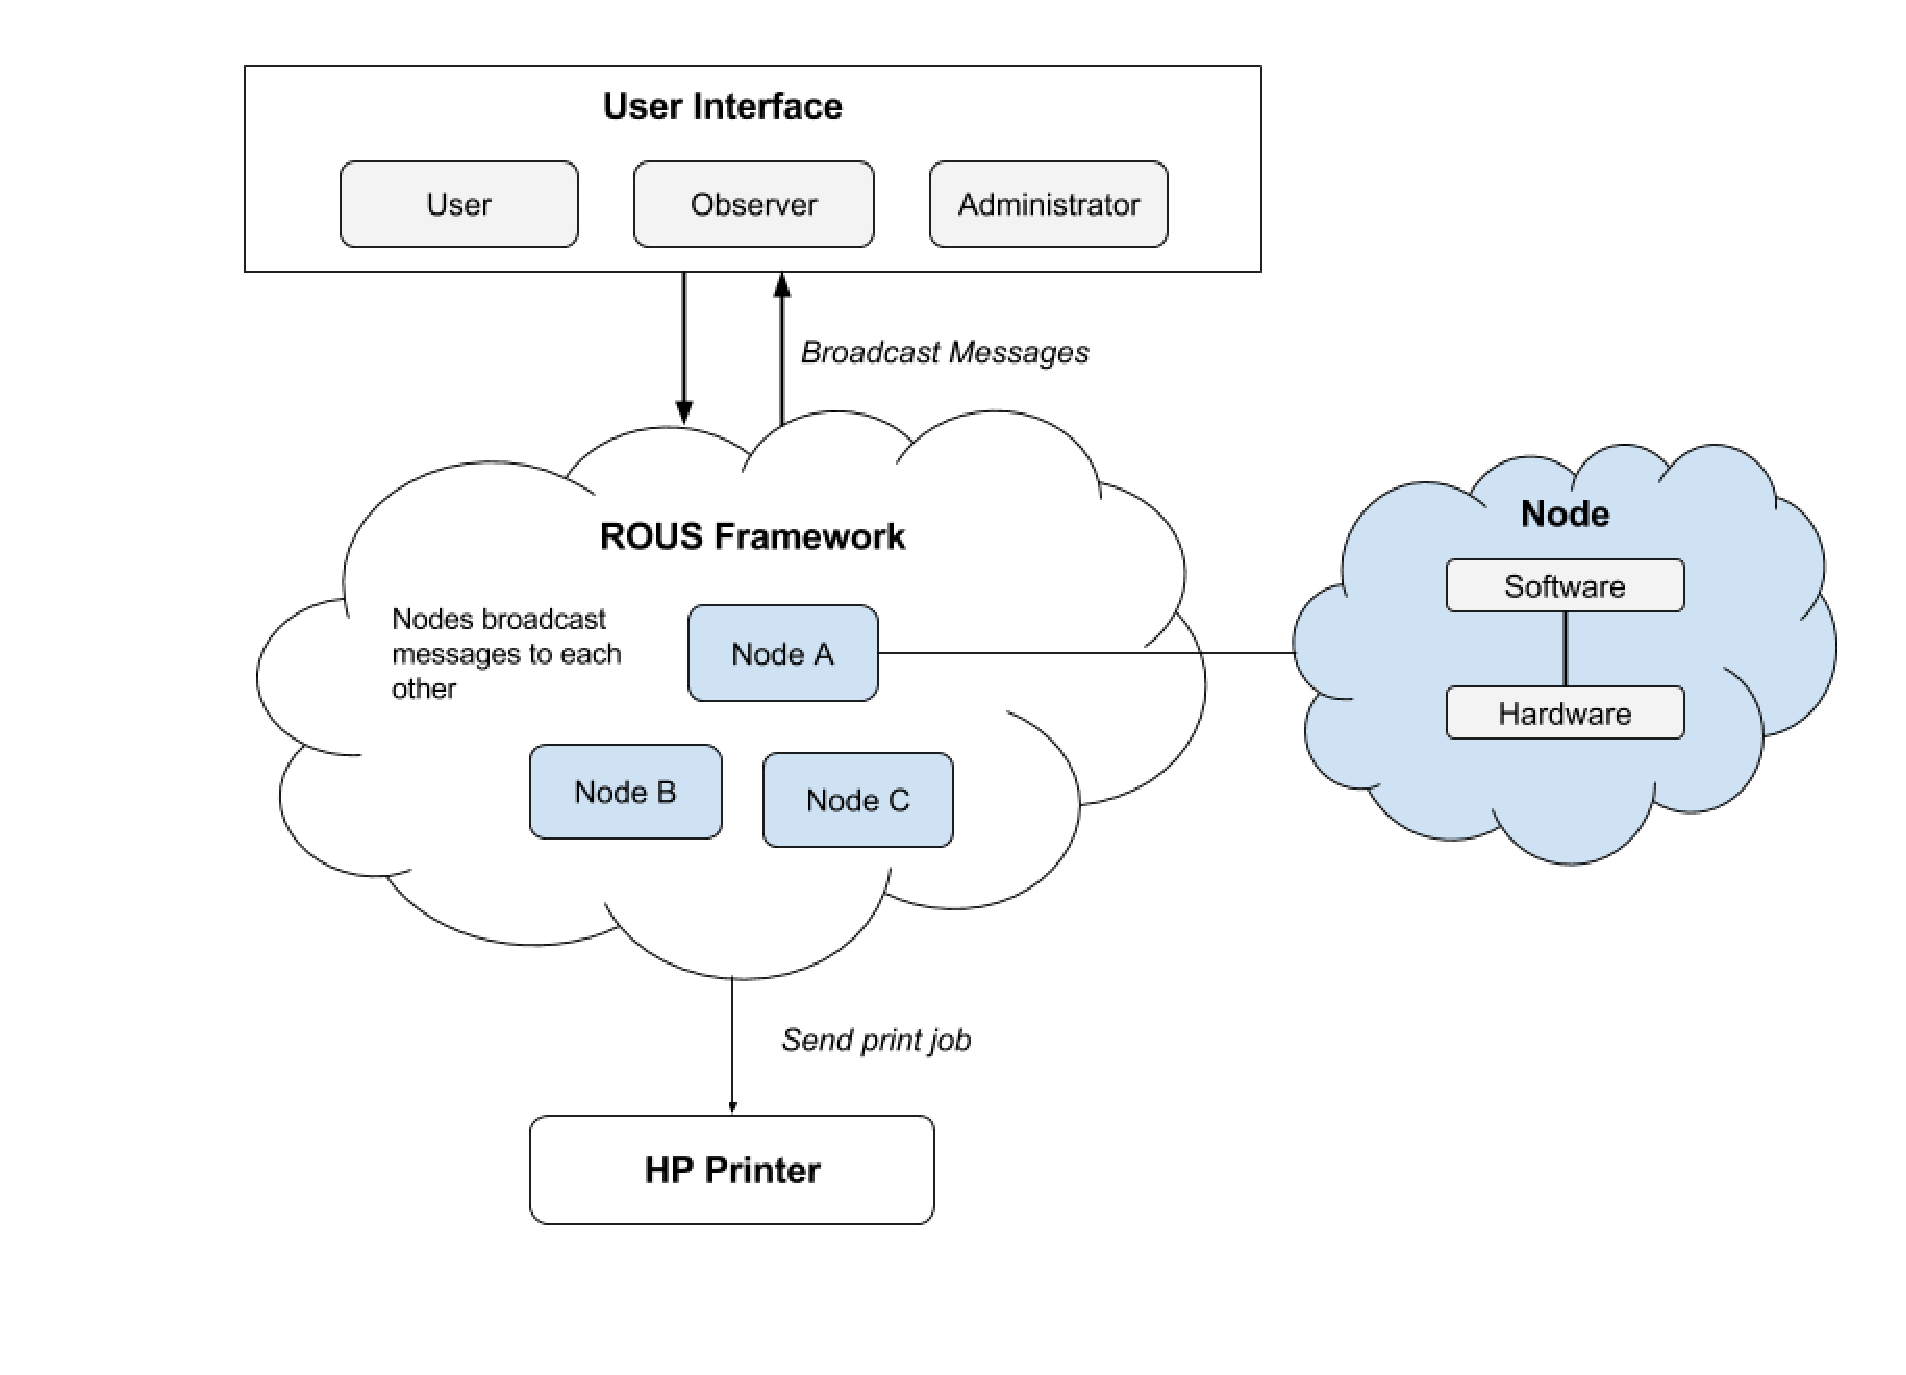
\includegraphics[scale=.45]{context}
	\captionsetup{justification=centering}
    \caption{This is a basic context view of the overall architecture of the ROUS framework}
\end{figure}

% \subsubsection{Rationale}
% Overall the rationale for the entire framework is to have a collection of loosely coupled nodes that can self organize to accomplish a print job. This framework will be robust in the face of any nodes that become untrusted. Nodes in this framework will communicate with each other using a complex language of messages over wireless Internet protocols. 

\subsubsection{Actors}
\paragraph{User}
Users only care about the ability to input a print job objective and have that printed output appear on their printers. They will not care about how the framework accomplishes these goals. These end users will not have the ability to affect the framework in any way other than inputting a print job and viewing the results.

\paragraph{Administrator}
Administrators perceive the framework in a different light than a user. These end users have the ability to see a more detailed look at the configuration and status of the framework. They also have the capabilities of seeing all services that each node offers and to disable those services. By disabling services these administrators are the end users who introduce sources of mistrust into the framework.

\paragraph{Observer}
An observer is someone that wants to see how the framework works. These end users will be able to see configuration setting and the state of the system. They will also be able to see all the nodes on the network and their services, and be able to see the state of those services.

\subsection{Software}
\subsubsection{Overview}
Our software framework will be built on top of a Linux kernel using hardware that will allow our framework to have access to wireless network protocols. Overall, this software framework will enable nodes to self organize on objectives without the need for any rigid logical configurations. The subsections below will take a detailed look at how nodes will communicate, what capabilities each node will have, and give an examination of what a source of mistrust means to the system.

\subsubsection{Node Communication}
\paragraph{Network Communication}
Basic node communication will happen over a partial ad hoc wireless network. A partial ad hoc network will be used because nodes will only be directly connected to each other when accessing print job objectives from other nodes. Most communication will happen via broadcasting a simple messages that each node will understand.

To accomplish network communication the framework will leverage two different transport network protocols, TCP and UDP. The protocol TCP will be used to transfer objective print job data from node to node. This protocol will be used because it will allow the framework to guarantee that packets will be delivered successfully and without error. 

In order to allow nodes to broadcast to multiple nodes at once, the framework will need to be able to use multi-cast. TCP does not allow multi-cast so the UDP transport protocol will be used for this feature. The framework will leverage the UDP protocol so that each node can broadcast a message to all nodes in the network. 

\paragraph{Broadcasting}
Broadcasting will be the most important feature in how nodes communicate with other nodes. Since the goal is to design a framework that is loosely coupled, nodes will almost never be directly connected to each other in a tightly coupled way. To solve this issue, nodes will only communicate by broadcasting simple messages to each other.

Each node will have the ability to broadcast messages to any node in the network. These nodes will also be able to listen for messages that were broadcast. They will send response messages. This is how basic communication works, a simple message that contains a print job objective is broadcast to all nodes. If a node can perform that objective it will response with a bid. The original node who sent the original message will then send the objective to the node that won the bid. 

The figure below illustrates how this sequence of message passing works.

% In the basic sense this communication will work as such, node one broadcasts message A, all other nodes listen to message A, assume node two meets the requirements message A calls for, then node two will respond via broadcast with message B. Node one listens and sees that node two responded with message B which then tells node one to either complete an objective or respond again with a new message C. This process will repeat until the print job objective has been successfully completed.
\begin{figure}[H]
\centering
	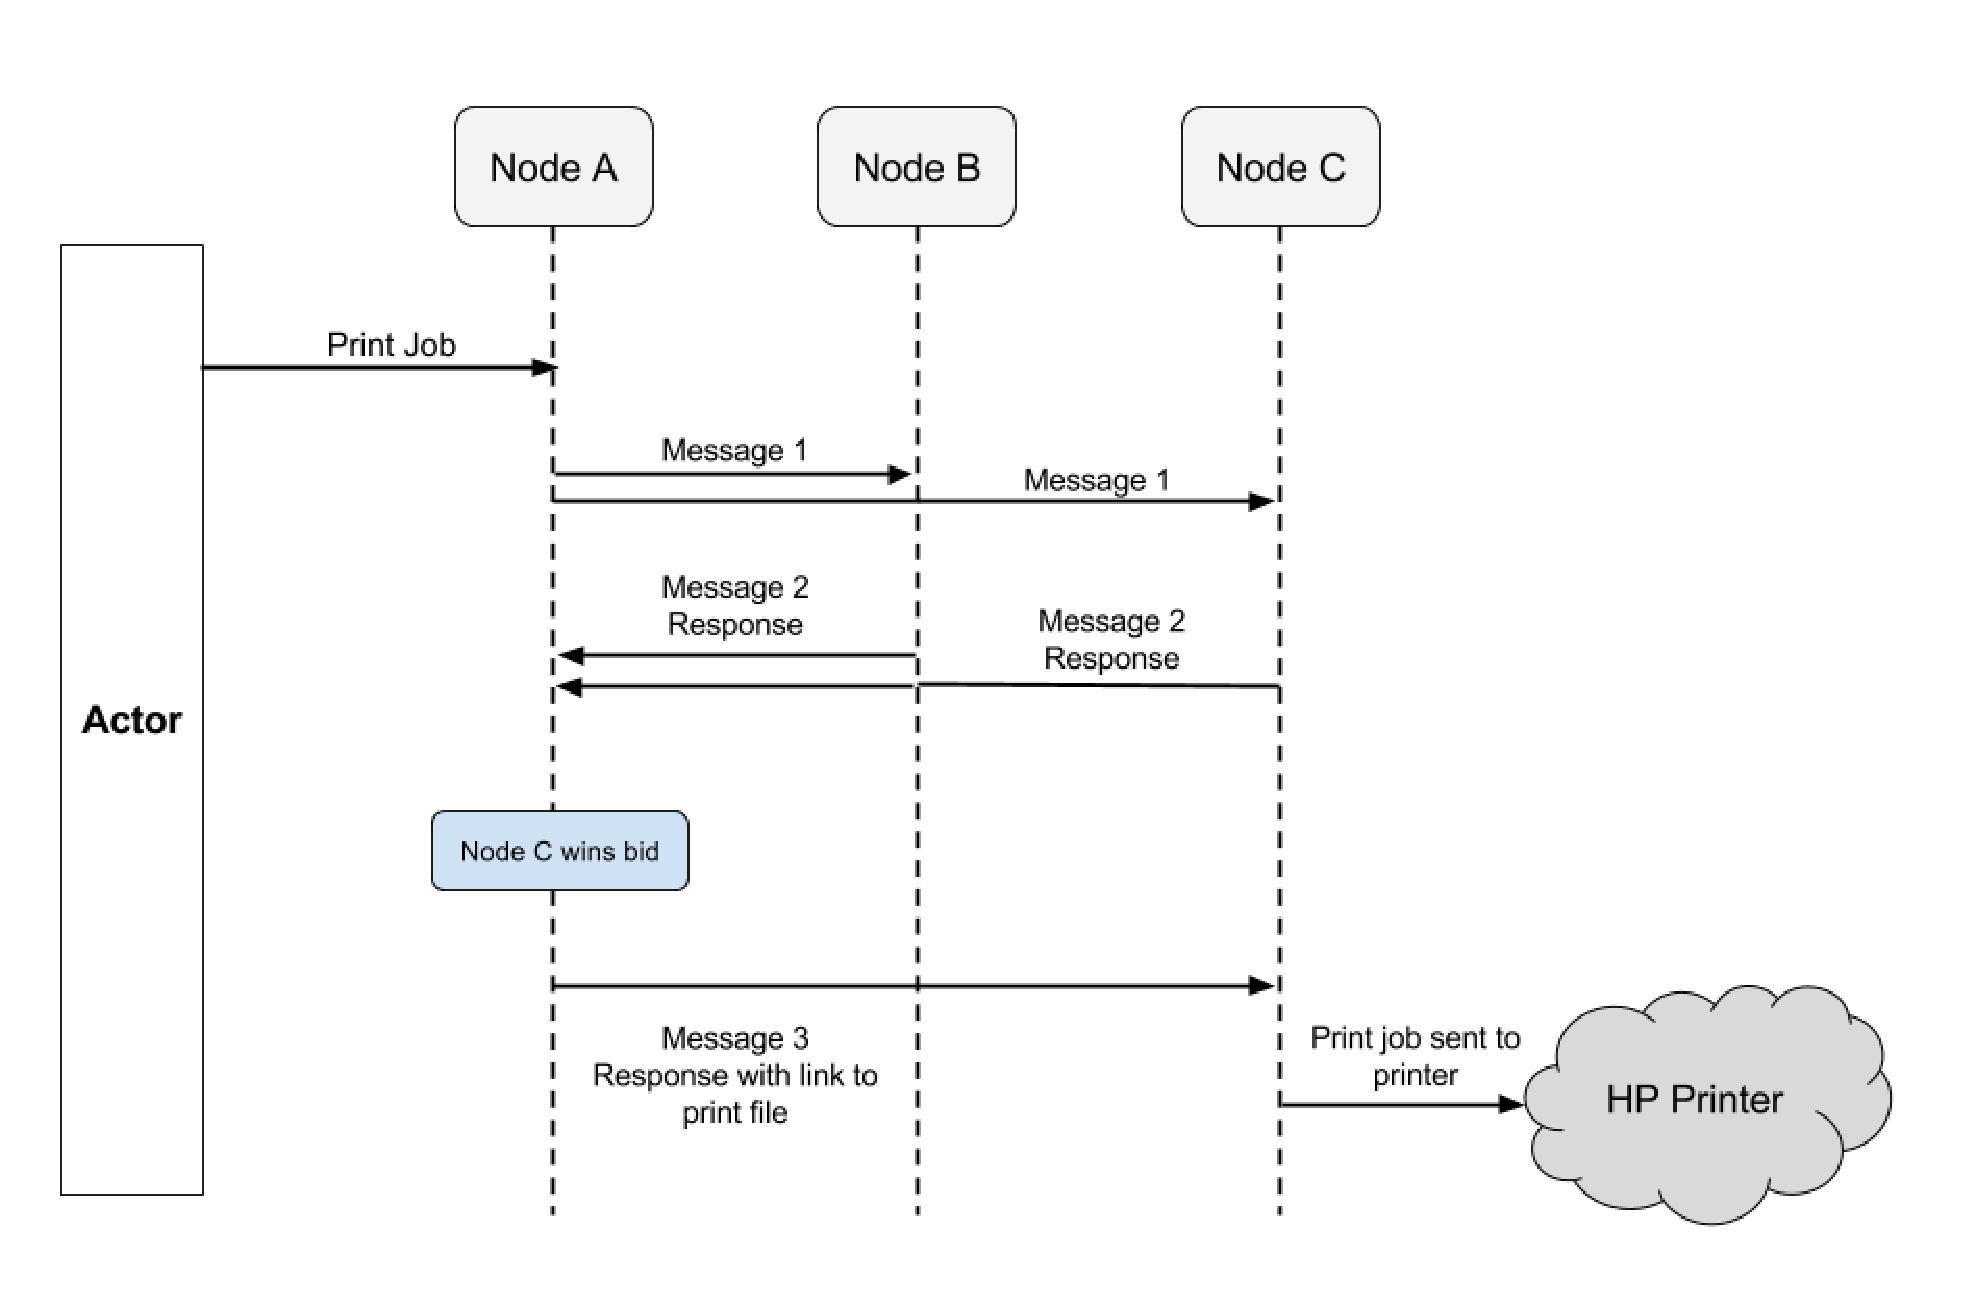
\includegraphics[scale=0.4]{sequence}
	\captionsetup{justification=centering}
    \caption{This illustrates a simple interaction between three nodes with the objective of printing a print job}
\end{figure}

\paragraph{Messages}
Simple message passing is the heart of how nodes will communicate to accomplish objectives. A simple message will contain a keyword, followed by the parameters that go with that keyword. Nodes will first look at a messages keyword to determine if they need to look for any parameters. 

As an example, a message will be sent with the keyword \textit{print} followed by the parameters \textit{color}. Any node that can first accept a \textit{print} keyword and then accept a \textit{color} parameter will response. All nodes will communicate using this simple message  \textit{keyword:parameter} format. 
% A complex language will be the heart of how nodes communicate with other nodes. When a node broadcasts messages, each message will be part of this complex language. Each node will know how to interpret this complex language in order for it to self organize and complete print job objectives.

% Overall, this language will be complex enough that each node will have no ambiguity about what is being asked, but it will also be simple enough that no rigid logical configurations exist on any nodes.


\subsubsection{Node Capabilities}
\paragraph{Services}
Every node in the framework will have a print job service. This print job service will give every node the ability to print an objective that has been inputted into the system. A service can be disabled by an administrator.

\paragraph{Bidding}
An important capability that each node will have is the ability to bid on services that it can complete. When another node broadcasts a message and more then one node responds, bidding then occurs. Each node will bid for the ability to be the node that is tasked with accomplishing the current print job objective. The node that one the bid will not be able to bid on new objective until it has completed the objective that it one the bid for. Nodes that lost the bid will then be available to bid on any new objective that is input in the framework.

% Each node has specific services it can complete. Some services may have subsections of the service; e.g. A printer service that can only print black and white. When a node receives the objective, it broadcasts asking for a bid number from the other nodes on the network that can complete the complex job. 
Once each node receives the broadcast for an objective, they will analyze the job and compare with it's own list of services it can accomplish. If the node can accomplish that service, it will record and broadcast a randomly generated number. Each node that can accomplish the service broadcasts their respective number. They will each compare their number with the others. If their number is larger than another nodes number, it will disregard the job and wait for the next objective. If there is not a number that is larger than that nodes generated number, that node will start fulfilling the objective.
% In the special case of a tie between the two nodes with the highest numbers, the two nodes will re-bid. Only these two nodes will rebid. This communication will be performed via multicast instead of broadcast. 	

\paragraph{File Interaction}
Objectives are print jobs in our framework. These print jobs will be a structured file that has the ability to be read and be printed by a printer. Files will be hosted from an end users file system. Paths to these files will be inputted into a node in the framework by the simple message passing system. 

% When one of these files is input into the framework, the node it was input onto will then have the ability to host that file. It needs this ability so that other nodes that gain the bid to accomplish the goal of printing that file will need to have a place to access that file from the node that holds the file. 

\paragraph{GUI Interaction}
End users will interact with our system through a graphical user interface. This GUI will interact with the framework by passing messages into the system, just like nodes do. For end users to make use this GUI, it is assumed that they will have their own system with a web browser.


\subsubsection{Source of Mistrust}
\paragraph{Overview} 
Our framework is required to be robust and have the ability to self organize to achieve an objective. A source of mistrust will be used to disable or shutdown nodes in ordered to show that our system is robust and can self organize in a way that mitigates issues. An input print job objective will be able to accomplished its goal even when a previously trusted services has now become untrusted. This gives our framework the ability to to introduce a source of mistrust which will then allow the user or administrator to see that our system is robust and able to overcome node mistrust issues.

%  One of the requirements for the system is to be able to mitigate a threat, but not have to detect it. To accomplish the mitigation of a threat, the network of nodes needs to have the ability to introduce a threat in some way shape or form. There need to be a way to introduce a threat to allow the observer to see that even with a threat introduced our system can mitigate it.
% The best way to introduce a simulated but realistic threat is to introduce the threat as if it was an objective. To create a Trojan of sorts that will "sneak" into the system and disrupt some services provided by nodes. This disruption will target a specific service and make the service unusable for only the node that wins the bid for the job. This will allow us to send an objective into the system that requires the disabled service and show that the system will still be able to complete the objective despite the node that has a disrupted service.

\paragraph{Effects}
This source of mistrust will simply be an administrator targeting a specific service on a specific node and disabling that service. Using the administrator interface will allow the end user to make a service unusable, which will show that objectives are completed despite a disrupted service.

Disabling a service will force a node that once was able to use a service, to no longer be able to use it. Once a service is disabled on a node, it can no longer bid for that service.

\paragraph{Organization}
By having the ability to introduce these sources of mistrust allows both the user and administrator to see that our framework is robust. It will show that nodes can self organize in order to accomplish an objective.

As an example, we have nodes one, two, and three. In the first situation node one broadcasts that it has a print job A. Node two and three respond that they can both handle the printing of print job A. They both bid and node two wins the bid. Node two then completes print job A. Next an administrator disables the print services offered by node two. The second situation starts the same, node one broadcasts that it has a print job A. This time though only node three responds that it can complete this print job and goes on to complete the objective. Thus we have shown that our system is robust and can self organize in the face of a source of mistrust and still complete the objective.
			




\subsection{Hardware}
\subsubsection{Overview} 
In order to build and deploy our software framework it will need a hardware platform to be built on top of. Our software framework will be built using a Linux kernel and the hardware will have wireless network capabilities. 

\subsubsection{Raspberry Pi}
A Raspberry Pi is a cheap, low powered, and cost effective replacement for having a full computer. This device can run an operating system, output video to a screen, output audio, and allow the connection of other peripherals. There small form factor makes it ideal for our software framework.

\subsubsection{Resin.io}
In conjunction with the Raspberry Pi we will use a third party framework to streamline the deployment of code to multiple devices. The Resin.io framework enables us to setup one Raspberry Pi and then deploy that code to all the other Raspberry Pi nodes. This allows us to have a single code base that gets deployed to all nodes when any changes are made. Overall this will greatly improve the ability to maintain code and for faster turn around times when updating the software features.




\subsection{Graphical User Interface}
\subsubsection{Overview}
Each end user will interact with the framework through a web based graphical user interface that is hosted by the framework. This interface will take the form of a single page web application that leverages front-end web toolkits in order to make development fast and efficient.

The GUI's goal will be different depending on the end user. Basic users will only have access to a component to input objectives into the framework and a component to see information about the status of inputted objectives. Administrators will have a components for each node of the network to enable and disable services. It will also contain components to see detailed framework configuration settings.
% The GUI will represent the main portion an end user would use to work with our product. The interface will be a Single Page Application written with a combination of basic web programming languages like HTML5, Cascading Style Sheets (CSS), and JavaScript (JS), specifically ReactJS. The interface will consist of one dynamic page that shows the nodal network, their respective services, and button for a user to input an objective.

% As the user first accesses the interface, a screen with the project logo and title will appear with the main graphic in the center showing each node currently in the system. Each node has a name or their IP address. 

\subsubsection{Toolkits}
In order to make the development of a web based GUI streamlined, our framework will use third party toolkits. ReactJS will be used to build the logic of the front end of the framework. It adds a quick and painless way to create interactive user interfaces, giving us extra features over using vanilla JavaScript. Bootstrap will give us a framework to make our user interface responsive and improve visuals.

\subsubsection{User Design}
\paragraph{Layout}
The layout for the user interface will consist of a graphical component to view the status of an objective, a button to select the print job objective, and a button to submit the objective into the system. When a print job is submitted by a user, the status will be displayed in the graphical component of the interface. This display will inform the user that their objective has been completed successfully. 
% The layout for our single page application consists of only two major points of interest; the main graphic and a button for the user to input an objective into the system. Of the two portions, the graphic will take up the most space. An image of the layout that the user could see is pictured below.
\begin{figure}[H]
\centering
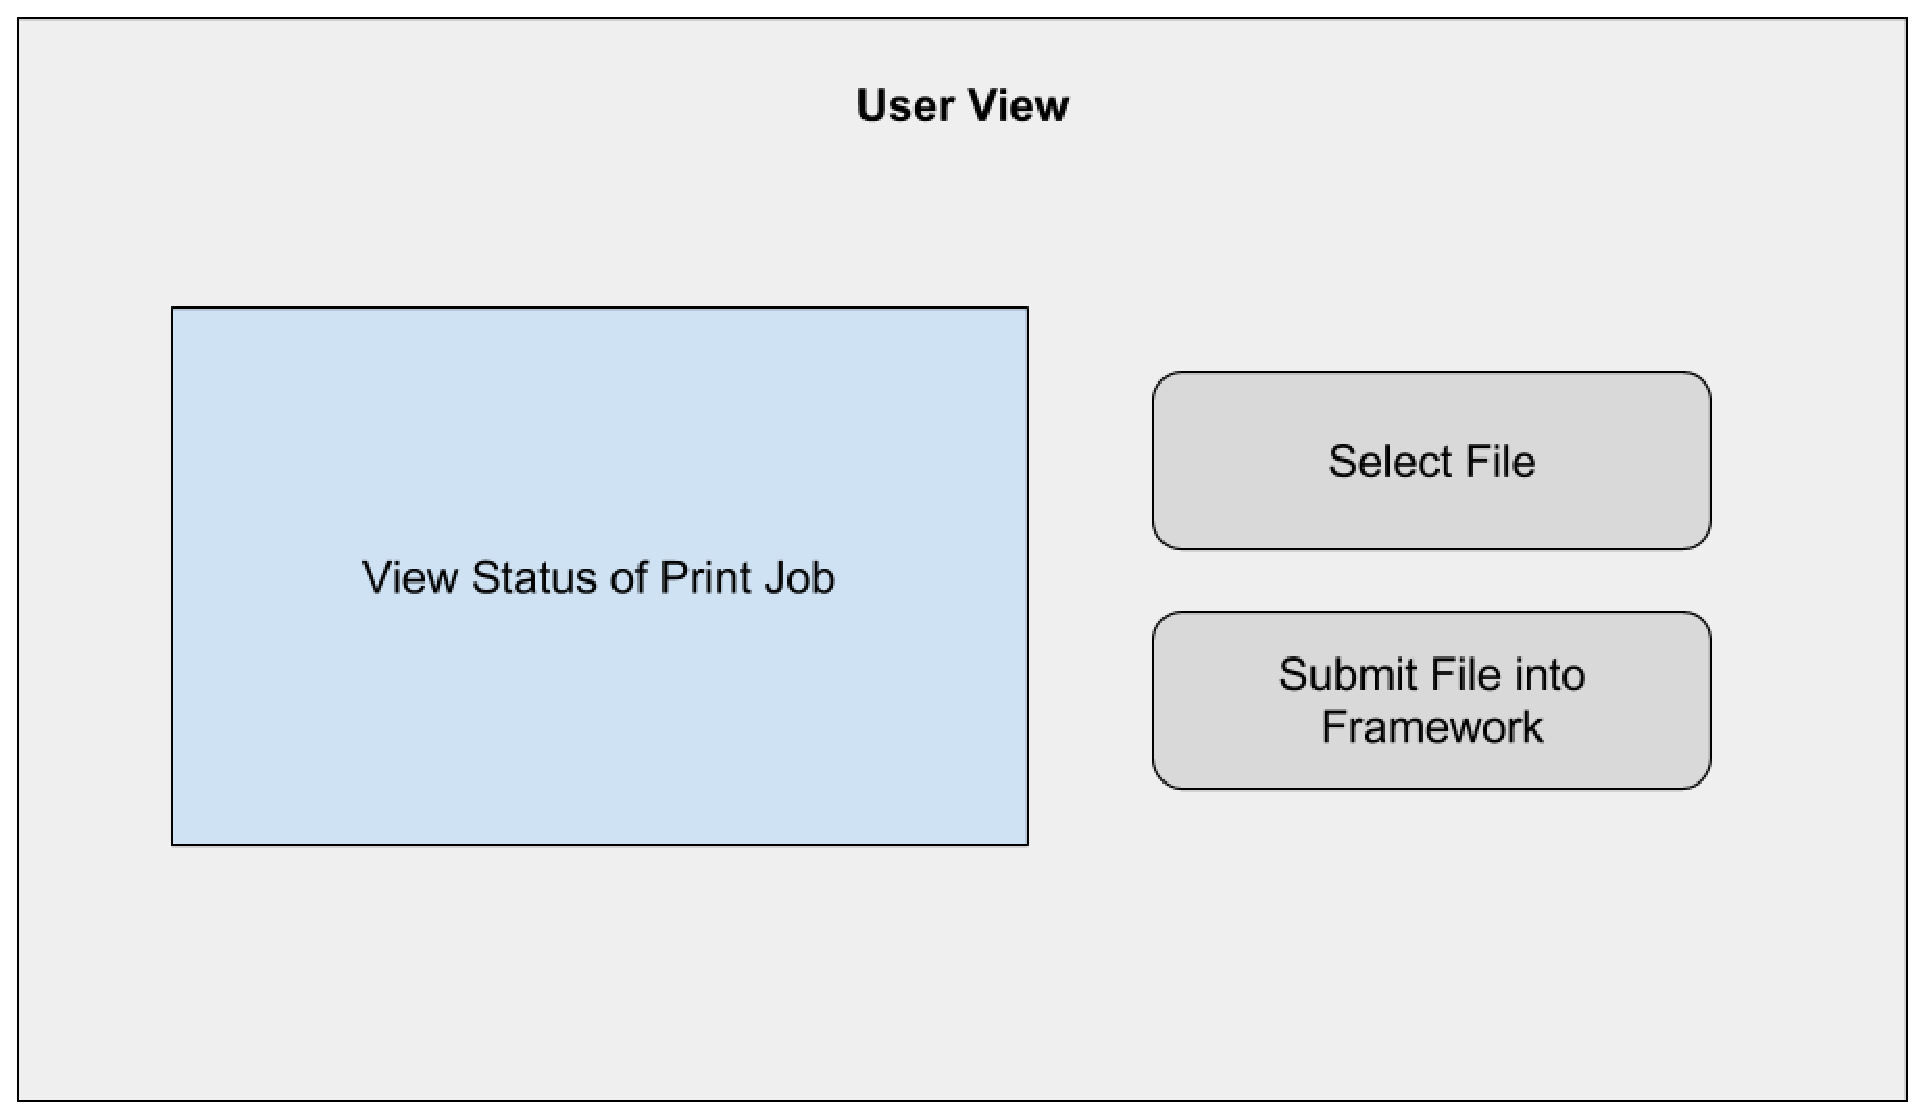
\includegraphics[scale=0.4]{user}
\captionsetup{justification=centering}
\caption{This figure shows a simple wire frame view of a user interface}
\end{figure}
% \paragraph{Graphic}
% A graphical representation of a node in the framework will display the current system state. This graphical representation will show the latest known nodes within the system, and the services they can perform. This graphic changes dynamically as nodes enter and exit the system. When one node is in a "busy" state while accomplishing a service, it is still shown in the diagram, but is slightly grayed out. A node will no longer appear in the system when there is no signal received from them after a timeout period. 
% \paragraph{Objective Input Button}
% Another portion of the main GUI is the objective input button. This button is for the user to pick a file to upload to the framework to be completed. Above the button is a text box with the filename of the file input. Once the file has been picked the user can choose to submit it into the system or cancel the submission.

\subsubsection{Observer Design}
An observer interface will include the ability for the observer to view detailed configuration and system state information. It will include the ability for these observers to see a list of all the nodes on the network, their status, and the services these nodes offer.
\begin{figure}
\centering
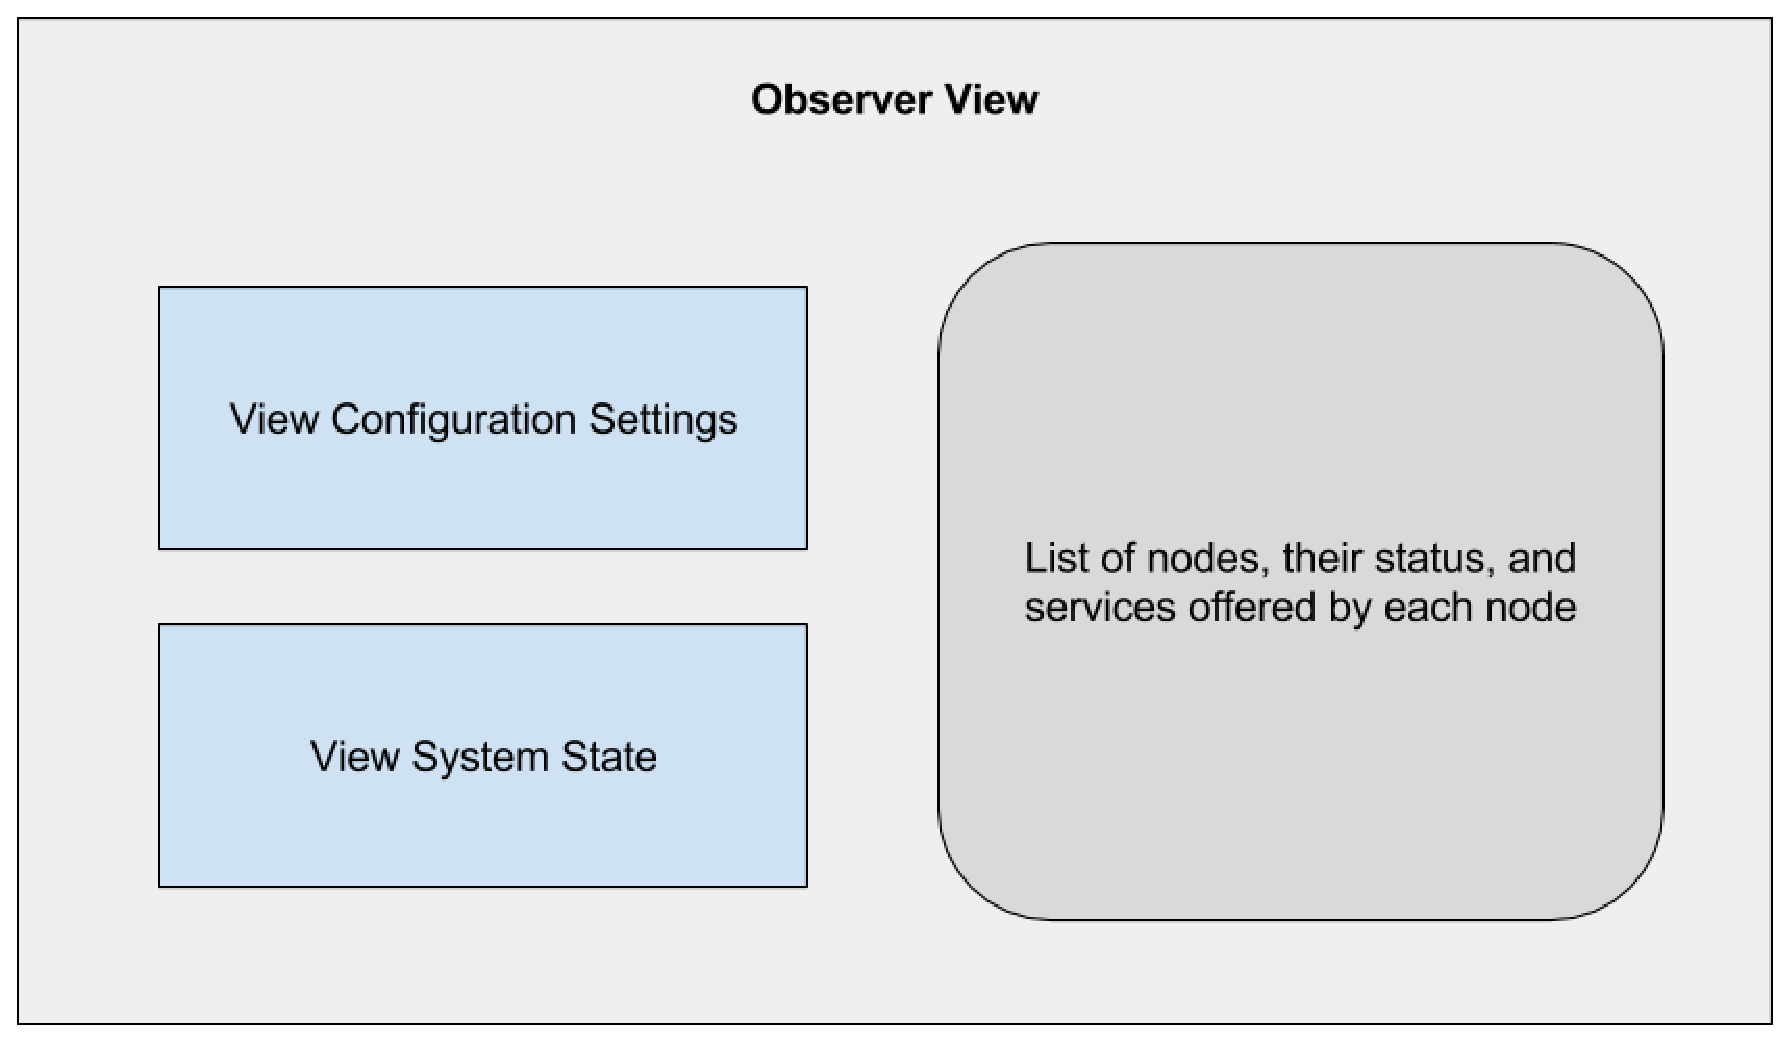
\includegraphics[scale=0.4]{observer}
\captionsetup{justification=centering}
\caption{This figure shows a simple wire frame view of an observer interface}
\end{figure}


\subsubsection{Administrator Design}
The administrator design is very similar to that of the observer, but the GUI contains more technical information and gives more options. Some of these different options include disabling services on different nodes by selecting the node, then selecting its respective service and clicking on a disable button. The disable button will disable currently disabled services the node is capable of doing and enable currently disabled services the node is capable of doing. 
The administrator would need to access the administrators web page by connecting to a different port of the same IP address.  
\begin{figure}[H]
\centering
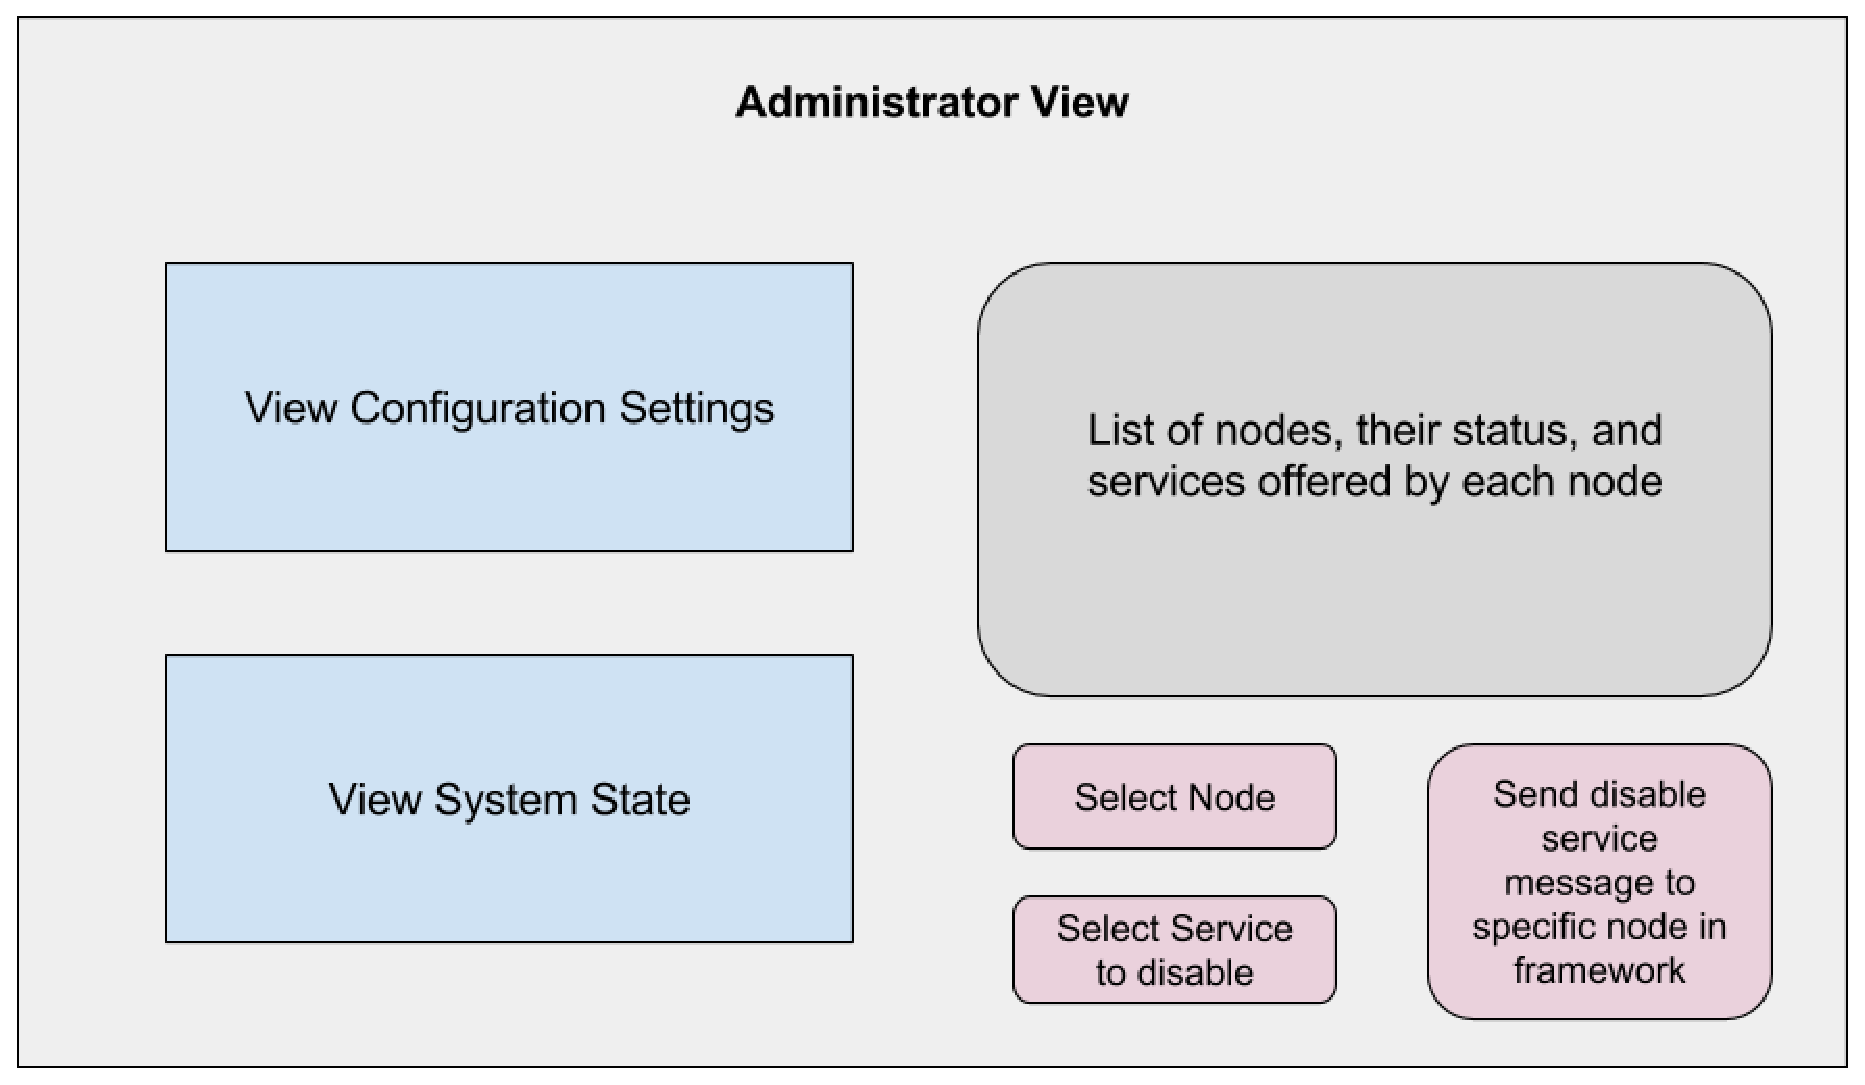
\includegraphics[scale=0.4]{admin}
\captionsetup{justification=centering}
\caption{This figure shows a simple wire frame view of the administrator interface}
\end{figure}




\subsection{Summary}
This framework will create a network of loosely coupled nodes that will communicate using a simple messages. It will enable users to input print job objectives into our framework and view the results from a graphical user interface. Nodes will be robust in the face of any mistrusted node. By being a robust framework, it will be able to accomplish objectives without each node having rigid logical configurations. The framework will use a combination of software and hardware. This software will contain core framework functionality, along with the graphical user interface. In the end, this framework will use a combination of software and hardware to enable a collection of wireless, loosely coupled nodes, to self organize on an objective.

%%%%%%%%%%%%%%%%%%%%%%%%%%%%%%%%%%%%%%%%%%%%%%%%%%
\subsection{Final Gantt Chart}


\begin{landscape}
 \begin{figure}[H]
  \centering
  \includegraphics[scale=0.25]{ROUS_Final_Gantt}
  \captionsetup{justification=centering}
  \caption{This is the final gantt chart for the project as a whole.}
  \label{fig:label}
 \end{figure}
\end{landscape}

\section{Design Document}
\subsection{Original}
%%%%%%%%%%%%%%%%%%%%%%%%%%%%%%%%%%%%%%%%%%%%%%%%%%


\subsection{Introduction}
\subsubsection{Overview}
The framework being developed will create a network of nodes that will communicate by broadcasting simple messages to each other. Nodes will use network protocols to pass these messages in order to self organize on an objective. Users will be able to input print job objectives into our framework and view the results from a graphical user interface.

Sections below take an in depth look at the design of the framework. These sections begin by taking a high level look at the overall design and then go into the specifics of how each piece of the framework is working together to accomplish an objective.

\subsubsection{Purpose}
Overall the rationale for the entire framework is to have a collection of loosely coupled nodes that can self organize to accomplish a print job. This framework will be robust in the face of any nodes that become untrusted. Nodes in this framework will communicate with each other using simple messages over wireless network protocols. 
% Our framework's purpose is to enable a collection of loosely coupled nodes to be robust in the face of any mistrusted node. The framework will give these nodes the ability to self organize on an objective. It will allow the input of a structured print job objective and will be able to self organize to accomplish that objective. This robust framework will be able to accomplish objectives without each node having rigid logical configurations.
% The purpose of this document is to give details on the design of the ROUS framework. By the end of this document, the reader will understand the concepts needed to create an IoT framework that will perform robustly and collaborate.

\subsubsection{Scope}
The scope of this project will includes using a combination of software and hardware to develop a framework for passing messages between a collection of loosely coupled nodes. Software will contain core framework functionality along with the graphical user interface. 

\subsubsection{Audience}
The intended audience is our client and mentor, Lonnie Mandigo. It also includes the professors of our senior design capstone class, Kirsten Winters and Kevin McGrath.

\subsubsection{Glossary}
\paragraph{Definitions, Acronyms, Abbreviations}
\bgroup
  \def\arraystretch{1.5}
  \resizebox{\textwidth}{!}{
  \begin{tabular}{| p{11.0cm} | p{11.0cm} |}
  \hline	
  \bf{Term} & \bf{Definition}\\
  \hline
  Node & The physical device that makes a piece of our network and provides functionality that can be applied to a variety of tasks\\
  \hline
  GUI & Graphical user Interface \\
  \hline
  TCP & Transmission Control Protocol: IP protocol that allows for reliable connection oriented communication between nodes \\
  \hline
  UDP & User Datagram Protocol: IP protocol that allows for connectionless communication between nodes  \\
  \hline
  Broadcast  & A networking signal to everyone on a network \\
  \hline
  Multicast & A networking signal to many destinations on the network \\
  \hline
  Raspberry Pi & A physical small form-factor platform used to hold our framework \\
  \hline
  Resin.io & Framework to help maintain and deploy code to Internet of things devices \\
  \hline
  ReactJS & A set of libraries for the JavaScript programming language designed for creating single page applications\\
  \hline
  \end{tabular}
  }
\egroup




\subsection{Overall Framework Design}
\subsubsection{Architecture}
The ROUS framework being implemented will be organized into three parts: software, hardware, and a graphical user interface. These separate pieces will work together to make up the overall framework. This system will have the functionality to be given a print job objective, organize on that objective, and then accomplish that print job objective.

In this framework all communication happens by broadcasting simple messages. A user interface will provide users, observers, and administrators the ability to interact with the framework. The framework will contain a network of nodes that communicate by broadcasting simple messages. 
\begin{figure}[H]
\centering
	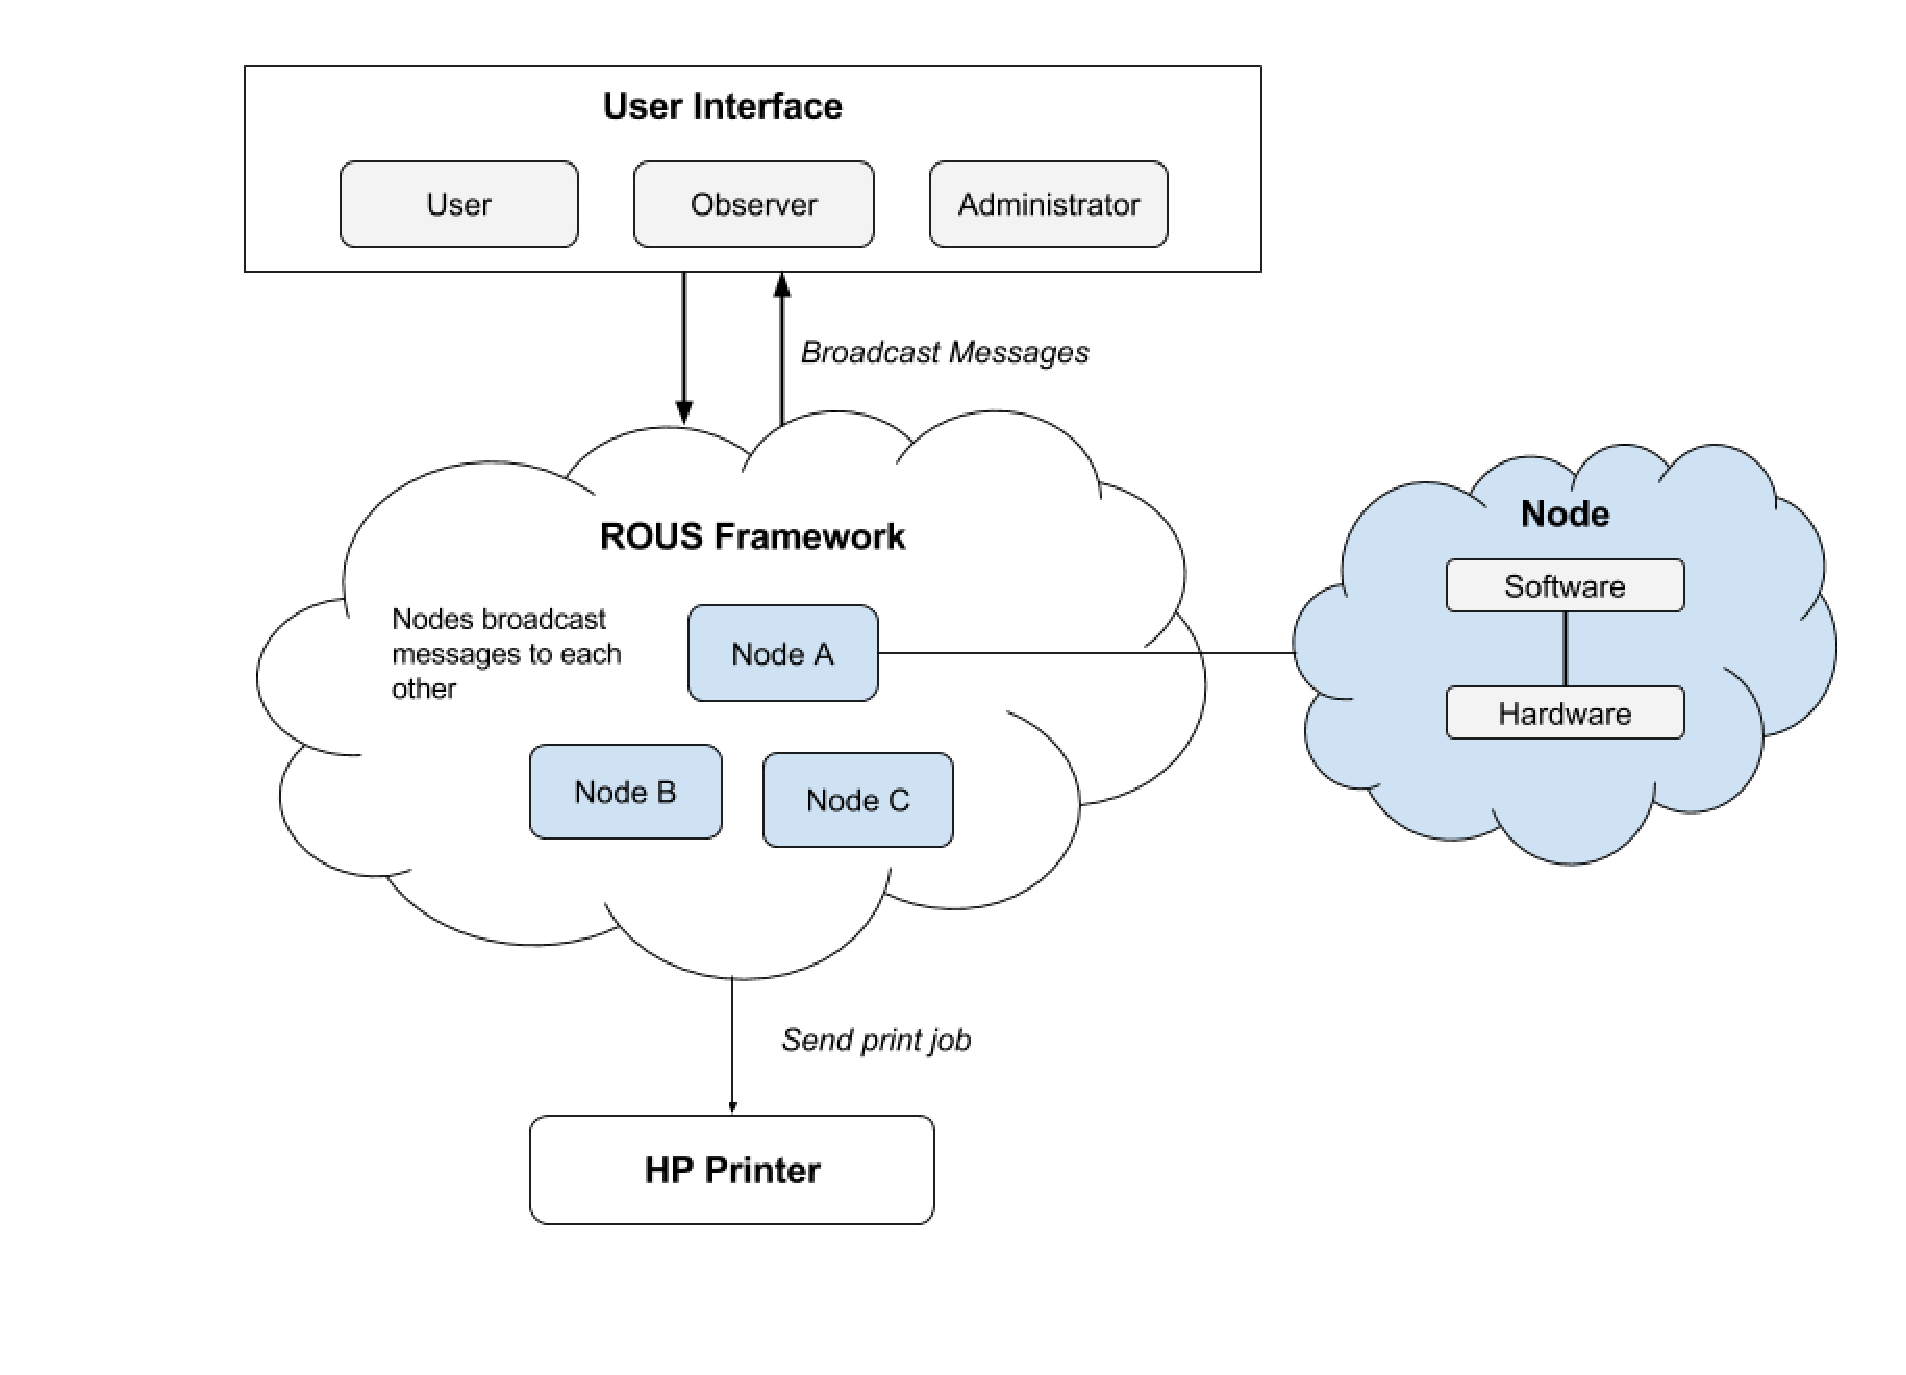
\includegraphics[scale=.45]{context}
	\captionsetup{justification=centering}
    \caption{This is a basic context view of the overall architecture of the ROUS framework}
\end{figure}

% \subsubsection{Rationale}
% Overall the rationale for the entire framework is to have a collection of loosely coupled nodes that can self organize to accomplish a print job. This framework will be robust in the face of any nodes that become untrusted. Nodes in this framework will communicate with each other using a complex language of messages over wireless Internet protocols. 

\subsubsection{Actors}
\paragraph{User}
Users only care about the ability to input a print job objective and have that printed output appear on their printers. They will not care about how the framework accomplishes these goals. These end users will not have the ability to affect the framework in any way other than inputting a print job and viewing the results.

\paragraph{Administrator}
Administrators perceive the framework in a different light than a user. These end users have the ability to see a more detailed look at the configuration and status of the framework. They also have the capabilities of seeing all services that each node offers and to disable those services. By disabling services these administrators are the end users who introduce sources of mistrust into the framework.

\paragraph{Observer}
An observer is someone that wants to see how the framework works. These end users will be able to see configuration setting and the state of the system. They will also be able to see all the nodes on the network and their services, and be able to see the state of those services.

\subsection{Software}
\subsubsection{Overview}
Our software framework will be built on top of a Linux kernel using hardware that will allow our framework to have access to wireless network protocols. Overall, this software framework will enable nodes to self organize on objectives without the need for any rigid logical configurations. The subsections below will take a detailed look at how nodes will communicate, what capabilities each node will have, and give an examination of what a source of mistrust means to the system.

\subsubsection{Node Communication}
\paragraph{Network Communication}
Basic node communication will happen over a partial ad hoc wireless network. A partial ad hoc network will be used because nodes will only be directly connected to each other when accessing print job objectives from other nodes. Most communication will happen via broadcasting a simple messages that each node will understand.

To accomplish network communication the framework will leverage two different transport network protocols, TCP and UDP. The protocol TCP will be used to transfer objective print job data from node to node. This protocol will be used because it will allow the framework to guarantee that packets will be delivered successfully and without error. 

In order to allow nodes to broadcast to multiple nodes at once, the framework will need to be able to use multi-cast. TCP does not allow multi-cast so the UDP transport protocol will be used for this feature. The framework will leverage the UDP protocol so that each node can broadcast a message to all nodes in the network. 

\paragraph{Broadcasting}
Broadcasting will be the most important feature in how nodes communicate with other nodes. Since the goal is to design a framework that is loosely coupled, nodes will almost never be directly connected to each other in a tightly coupled way. To solve this issue, nodes will only communicate by broadcasting simple messages to each other.

Each node will have the ability to broadcast messages to any node in the network. These nodes will also be able to listen for messages that were broadcast. They will send response messages. This is how basic communication works, a simple message that contains a print job objective is broadcast to all nodes. If a node can perform that objective it will response with a bid. The original node who sent the original message will then send the objective to the node that won the bid. 

The figure below illustrates how this sequence of message passing works.

% In the basic sense this communication will work as such, node one broadcasts message A, all other nodes listen to message A, assume node two meets the requirements message A calls for, then node two will respond via broadcast with message B. Node one listens and sees that node two responded with message B which then tells node one to either complete an objective or respond again with a new message C. This process will repeat until the print job objective has been successfully completed.
\begin{figure}[H]
\centering
	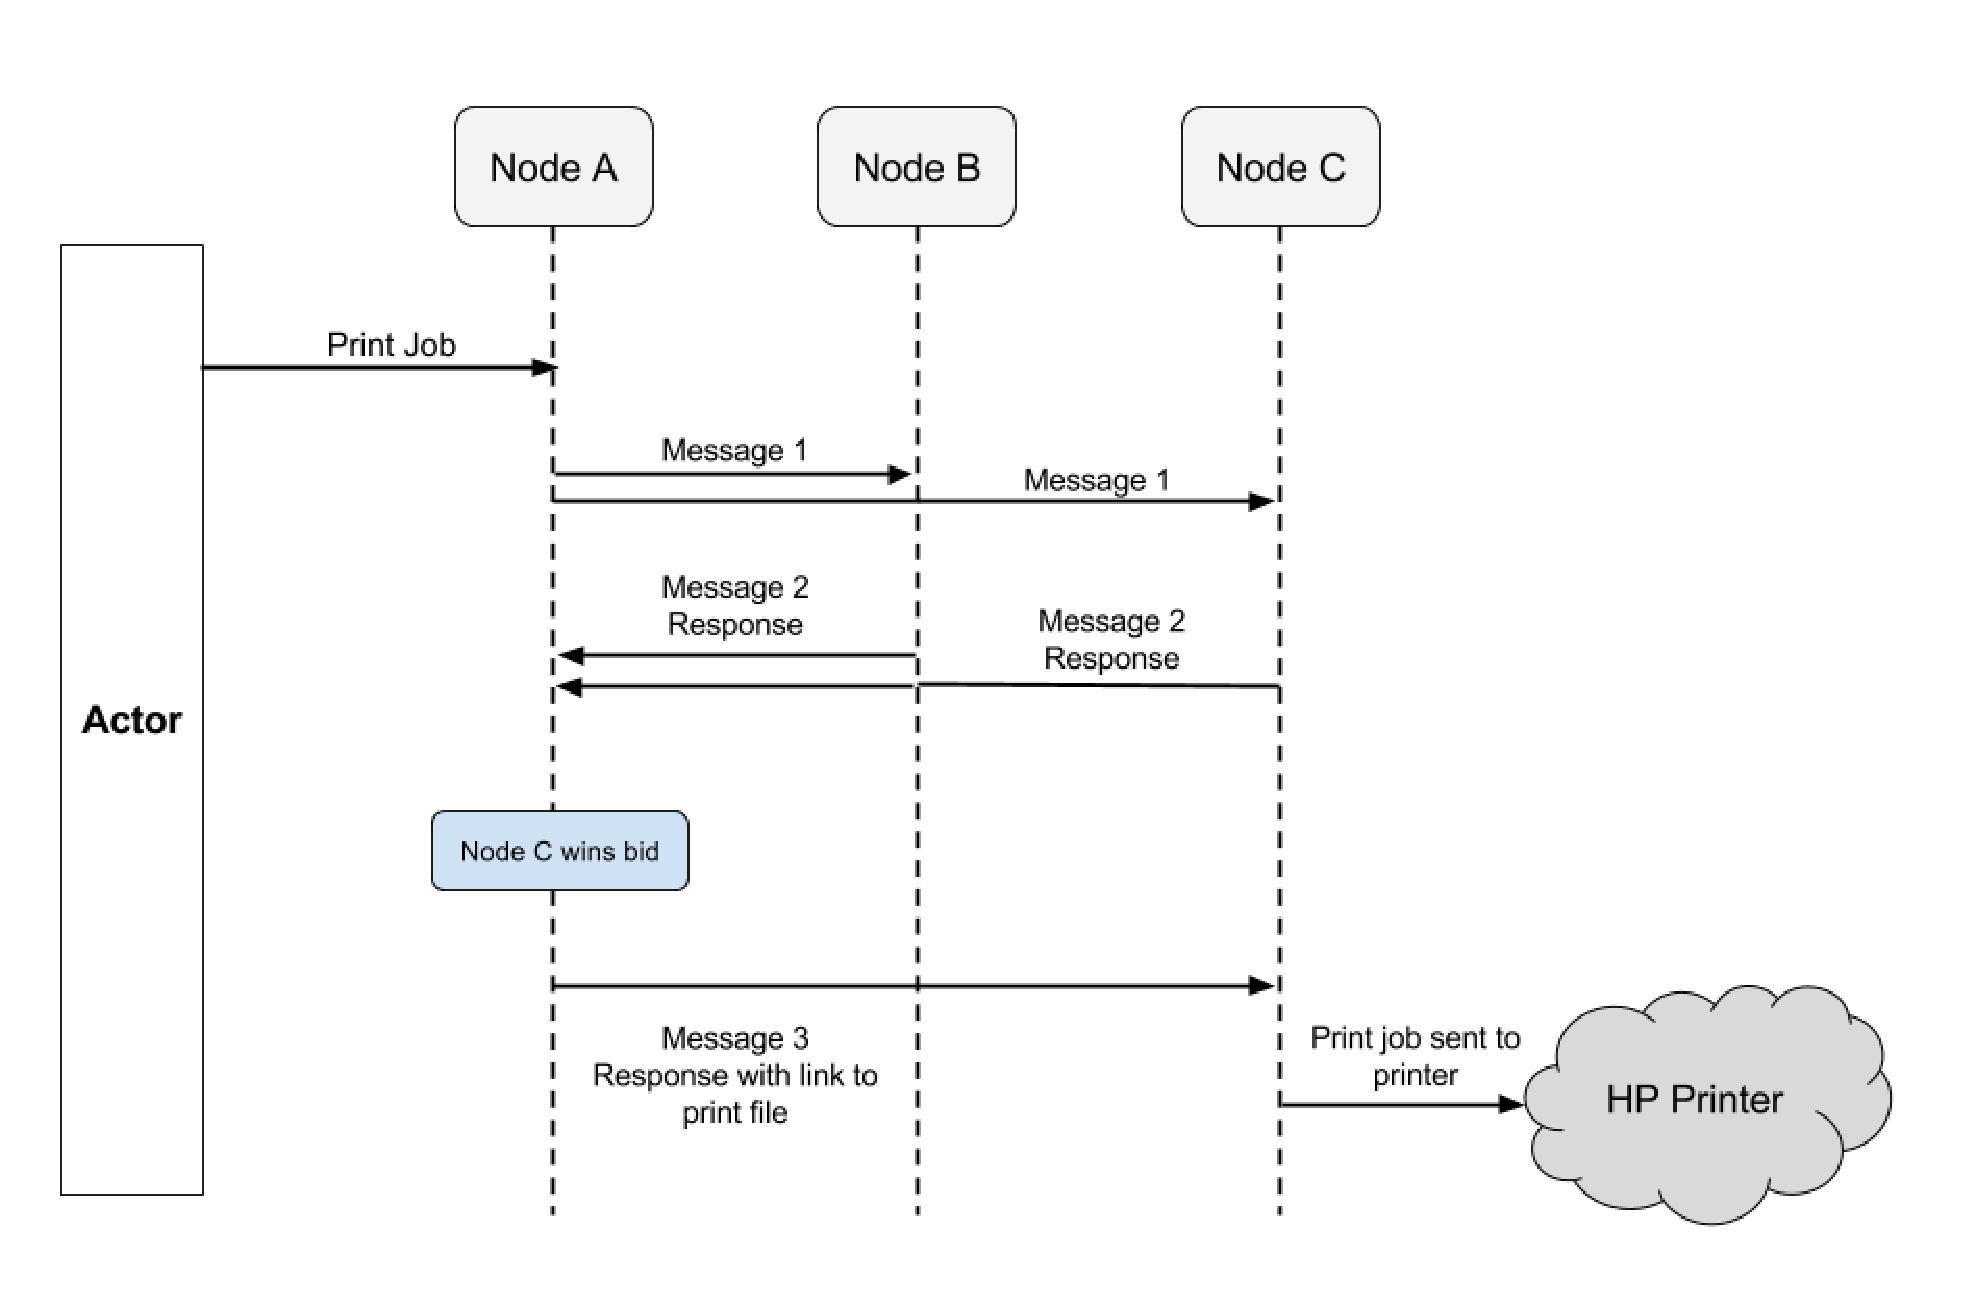
\includegraphics[scale=0.4]{sequence}
	\captionsetup{justification=centering}
    \caption{This illustrates a simple interaction between three nodes with the objective of printing a print job}
\end{figure}

\paragraph{Messages}
Simple message passing is the heart of how nodes will communicate to accomplish objectives. A simple message will contain a keyword, followed by the parameters that go with that keyword. Nodes will first look at a messages keyword to determine if they need to look for any parameters. 

As an example, a message will be sent with the keyword \textit{print} followed by the parameters \textit{color}. Any node that can first accept a \textit{print} keyword and then accept a \textit{color} parameter will response. All nodes will communicate using this simple message  \textit{keyword:parameter} format. 
% A complex language will be the heart of how nodes communicate with other nodes. When a node broadcasts messages, each message will be part of this complex language. Each node will know how to interpret this complex language in order for it to self organize and complete print job objectives.

% Overall, this language will be complex enough that each node will have no ambiguity about what is being asked, but it will also be simple enough that no rigid logical configurations exist on any nodes.


\subsubsection{Node Capabilities}
\paragraph{Services}
Every node in the framework will have a print job service. This print job service will give every node the ability to print an objective that has been inputted into the system. A service can be disabled by an administrator.

\paragraph{Bidding}
An important capability that each node will have is the ability to bid on services that it can complete. When another node broadcasts a message and more then one node responds, bidding then occurs. Each node will bid for the ability to be the node that is tasked with accomplishing the current print job objective. The node that one the bid will not be able to bid on new objective until it has completed the objective that it one the bid for. Nodes that lost the bid will then be available to bid on any new objective that is input in the framework.

% Each node has specific services it can complete. Some services may have subsections of the service; e.g. A printer service that can only print black and white. When a node receives the objective, it broadcasts asking for a bid number from the other nodes on the network that can complete the complex job. 
Once each node receives the broadcast for an objective, they will analyze the job and compare with it's own list of services it can accomplish. If the node can accomplish that service, it will record and broadcast a randomly generated number. Each node that can accomplish the service broadcasts their respective number. They will each compare their number with the others. If their number is larger than another nodes number, it will disregard the job and wait for the next objective. If there is not a number that is larger than that nodes generated number, that node will start fulfilling the objective.
% In the special case of a tie between the two nodes with the highest numbers, the two nodes will re-bid. Only these two nodes will rebid. This communication will be performed via multicast instead of broadcast. 	

\paragraph{File Interaction}
Objectives are print jobs in our framework. These print jobs will be a structured file that has the ability to be read and be printed by a printer. Files will be hosted from an end users file system. Paths to these files will be inputted into a node in the framework by the simple message passing system. 

% When one of these files is input into the framework, the node it was input onto will then have the ability to host that file. It needs this ability so that other nodes that gain the bid to accomplish the goal of printing that file will need to have a place to access that file from the node that holds the file. 

\paragraph{GUI Interaction}
End users will interact with our system through a graphical user interface. This GUI will interact with the framework by passing messages into the system, just like nodes do. For end users to make use this GUI, it is assumed that they will have their own system with a web browser.


\subsubsection{Source of Mistrust}
\paragraph{Overview} 
Our framework is required to be robust and have the ability to self organize to achieve an objective. A source of mistrust will be used to disable or shutdown nodes in ordered to show that our system is robust and can self organize in a way that mitigates issues. An input print job objective will be able to accomplished its goal even when a previously trusted services has now become untrusted. This gives our framework the ability to to introduce a source of mistrust which will then allow the user or administrator to see that our system is robust and able to overcome node mistrust issues.

%  One of the requirements for the system is to be able to mitigate a threat, but not have to detect it. To accomplish the mitigation of a threat, the network of nodes needs to have the ability to introduce a threat in some way shape or form. There need to be a way to introduce a threat to allow the observer to see that even with a threat introduced our system can mitigate it.
% The best way to introduce a simulated but realistic threat is to introduce the threat as if it was an objective. To create a Trojan of sorts that will "sneak" into the system and disrupt some services provided by nodes. This disruption will target a specific service and make the service unusable for only the node that wins the bid for the job. This will allow us to send an objective into the system that requires the disabled service and show that the system will still be able to complete the objective despite the node that has a disrupted service.

\paragraph{Effects}
This source of mistrust will simply be an administrator targeting a specific service on a specific node and disabling that service. Using the administrator interface will allow the end user to make a service unusable, which will show that objectives are completed despite a disrupted service.

Disabling a service will force a node that once was able to use a service, to no longer be able to use it. Once a service is disabled on a node, it can no longer bid for that service.

\paragraph{Organization}
By having the ability to introduce these sources of mistrust allows both the user and administrator to see that our framework is robust. It will show that nodes can self organize in order to accomplish an objective.

As an example, we have nodes one, two, and three. In the first situation node one broadcasts that it has a print job A. Node two and three respond that they can both handle the printing of print job A. They both bid and node two wins the bid. Node two then completes print job A. Next an administrator disables the print services offered by node two. The second situation starts the same, node one broadcasts that it has a print job A. This time though only node three responds that it can complete this print job and goes on to complete the objective. Thus we have shown that our system is robust and can self organize in the face of a source of mistrust and still complete the objective.
			




\subsection{Hardware}
\subsubsection{Overview} 
In order to build and deploy our software framework it will need a hardware platform to be built on top of. Our software framework will be built using a Linux kernel and the hardware will have wireless network capabilities. 

\subsubsection{Raspberry Pi}
A Raspberry Pi is a cheap, low powered, and cost effective replacement for having a full computer. This device can run an operating system, output video to a screen, output audio, and allow the connection of other peripherals. There small form factor makes it ideal for our software framework.




\subsection{Graphical User Interface}
\subsubsection{Overview}
Each end user will interact with the framework through a web based graphical user interface that is hosted by the framework. This interface will take the form of a single page web application that leverages front-end web toolkits in order to make development fast and efficient.

The GUI's goal will be different depending on the end user. Basic users will only have access to a component to input objectives into the framework and a component to see information about the status of inputted objectives. Administrators will have a components for each node of the network to enable and disable services. It will also contain components to see detailed framework configuration settings.
% The GUI will represent the main portion an end user would use to work with our product. The interface will be a Single Page Application written with a combination of basic web programming languages like HTML5, Cascading Style Sheets (CSS), and JavaScript (JS), specifically ReactJS. The interface will consist of one dynamic page that shows the nodal network, their respective services, and button for a user to input an objective.

% As the user first accesses the interface, a screen with the project logo and title will appear with the main graphic in the center showing each node currently in the system. Each node has a name or their IP address. 

\subsubsection{Toolkits}
In order to make the development of a web based GUI streamlined, our framework will use third party toolkits. ReactJS will be used to build the logic of the front end of the framework. It adds a quick and painless way to create interactive user interfaces, giving us extra features over using vanilla JavaScript. Bootstrap will give us a framework to make our user interface responsive and improve visuals.

\subsubsection{User Design}
\paragraph{Layout}
The layout for the user interface will consist of a graphical component to view the status of an objective, a button to select the print job objective, and a button to submit the objective into the system. When a print job is submitted by a user, the status will be displayed in the graphical component of the interface. This display will inform the user that their objective has been completed successfully. 
% The layout for our single page application consists of only two major points of interest; the main graphic and a button for the user to input an objective into the system. Of the two portions, the graphic will take up the most space. An image of the layout that the user could see is pictured below.
\begin{figure}[H]
\centering
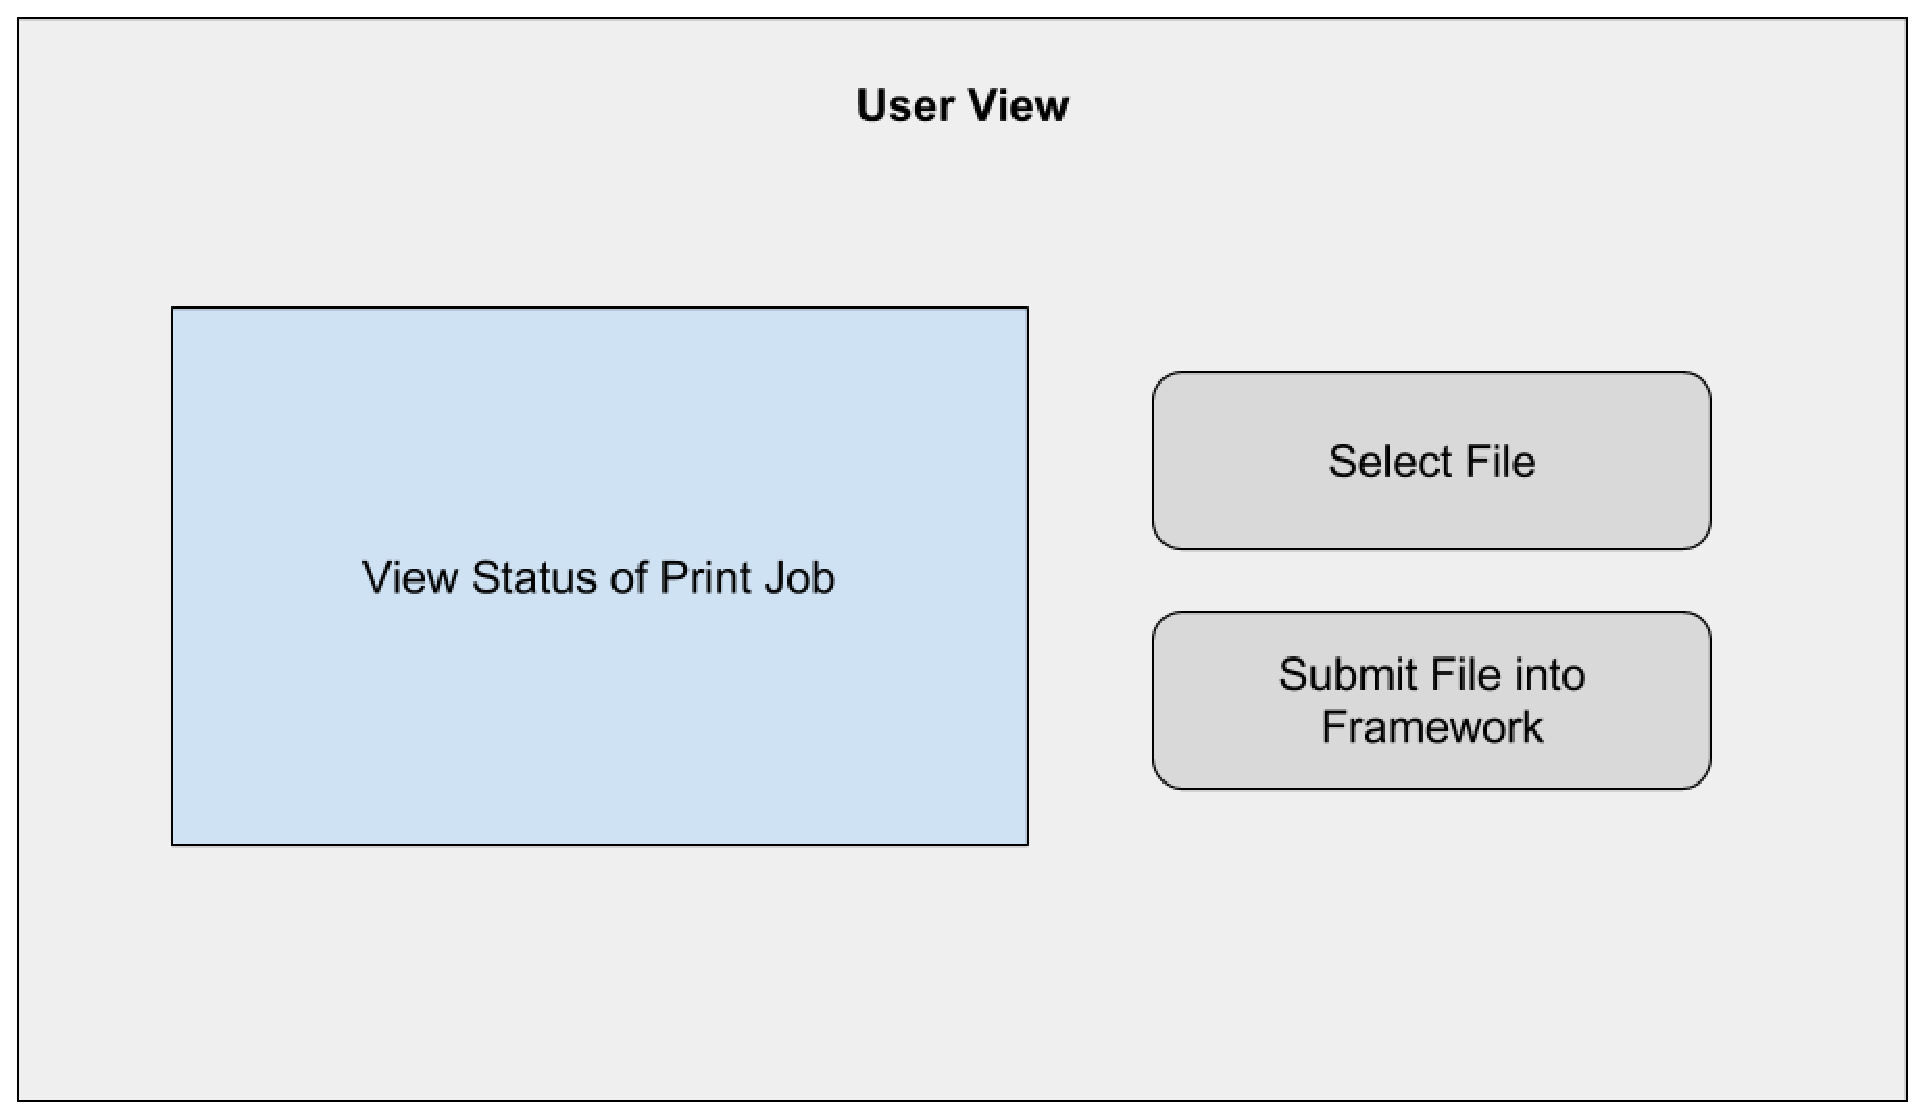
\includegraphics[scale=0.4]{user}
\captionsetup{justification=centering}
\caption{This figure shows a simple wire frame view of a user interface}
\end{figure}
% \paragraph{Graphic}
% A graphical representation of a node in the framework will display the current system state. This graphical representation will show the latest known nodes within the system, and the services they can perform. This graphic changes dynamically as nodes enter and exit the system. When one node is in a "busy" state while accomplishing a service, it is still shown in the diagram, but is slightly grayed out. A node will no longer appear in the system when there is no signal received from them after a timeout period. 
% \paragraph{Objective Input Button}
% Another portion of the main GUI is the objective input button. This button is for the user to pick a file to upload to the framework to be completed. Above the button is a text box with the filename of the file input. Once the file has been picked the user can choose to submit it into the system or cancel the submission.

\subsubsection{Observer Design}
An observer interface will include the ability for the observer to view detailed configuration and system state information. It will include the ability for these observers to see a list of all the nodes on the network, their status, and the services these nodes offer.
\begin{figure}[H]
\centering
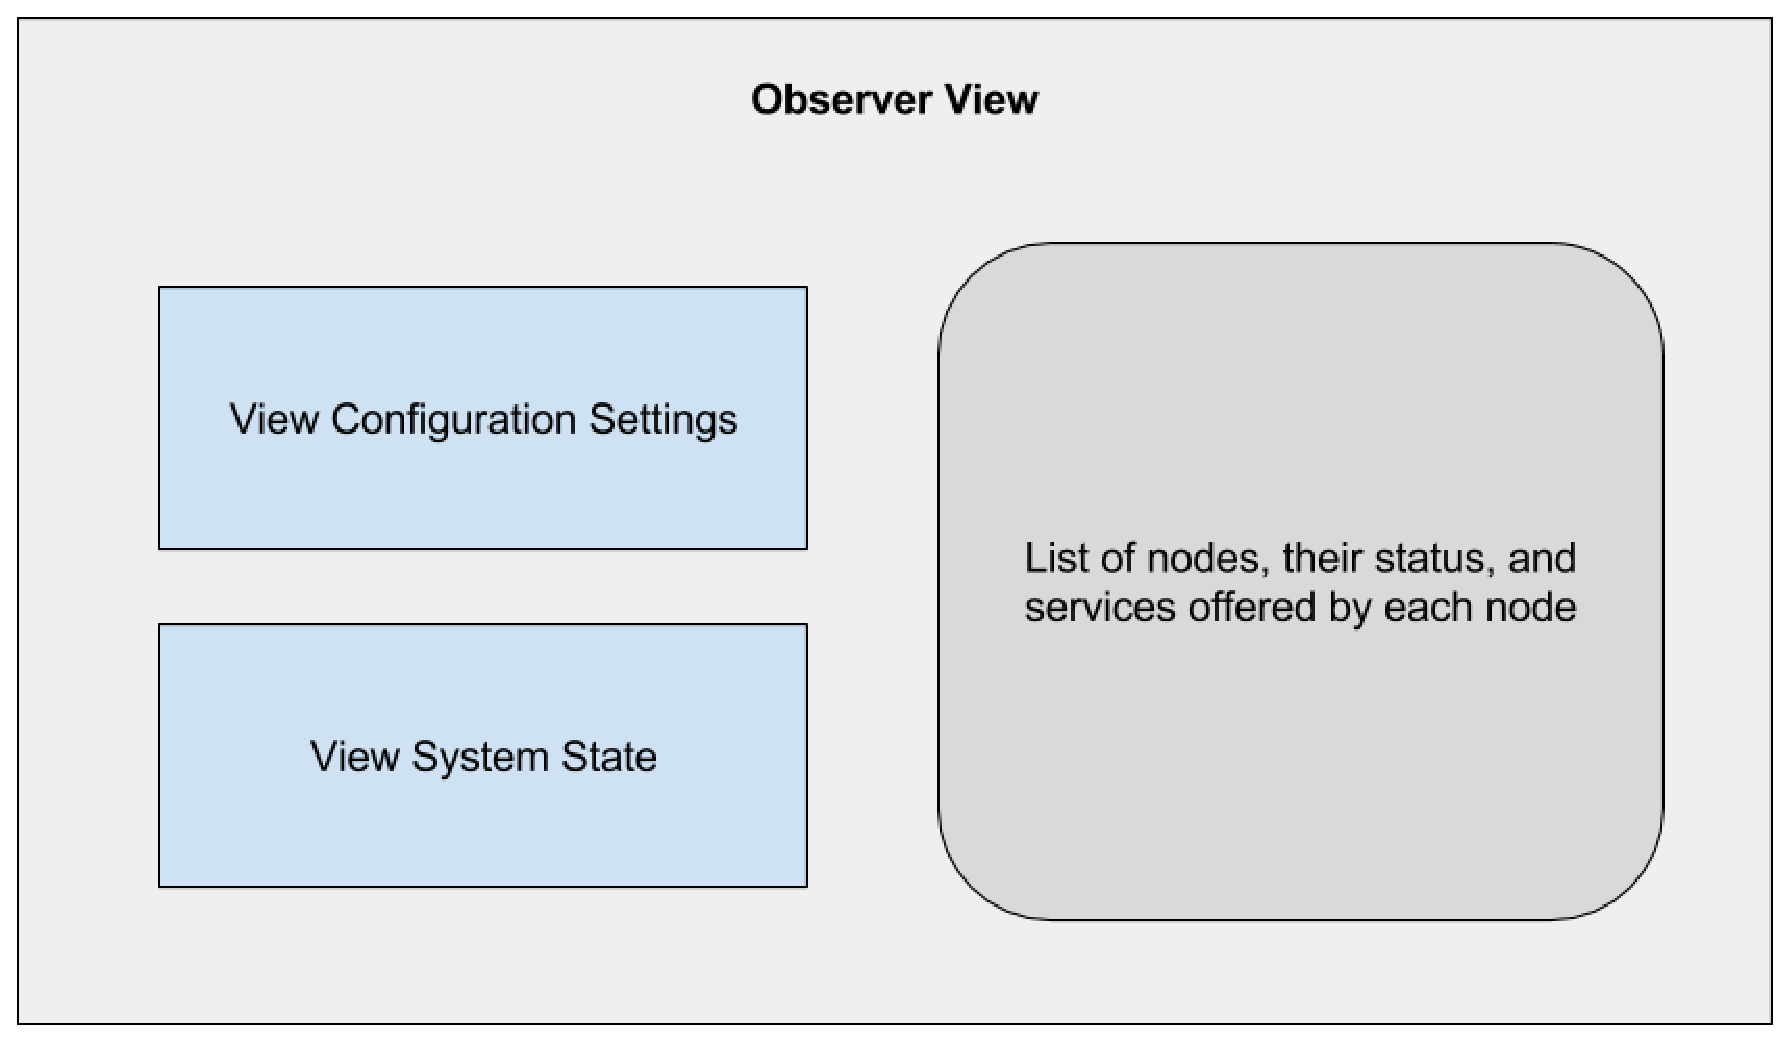
\includegraphics[scale=0.4]{observer}
\captionsetup{justification=centering}
\caption{This figure shows a simple wire frame view of an observer interface}
\end{figure}


\subsubsection{Administrator Design}
The administrator design is very similar to that of the observer, but the GUI contains more technical information and gives more options. Some of these different options include disabling services on different nodes by selecting the node, then selecting its respective service and clicking on a disable button. The disable button will disable currently disabled services the node is capable of doing and enable currently disabled services the node is capable of doing. 
The administrator would need to access the administrators web page by connecting to a different port of the same IP address.  
\begin{figure}[H]
\centering
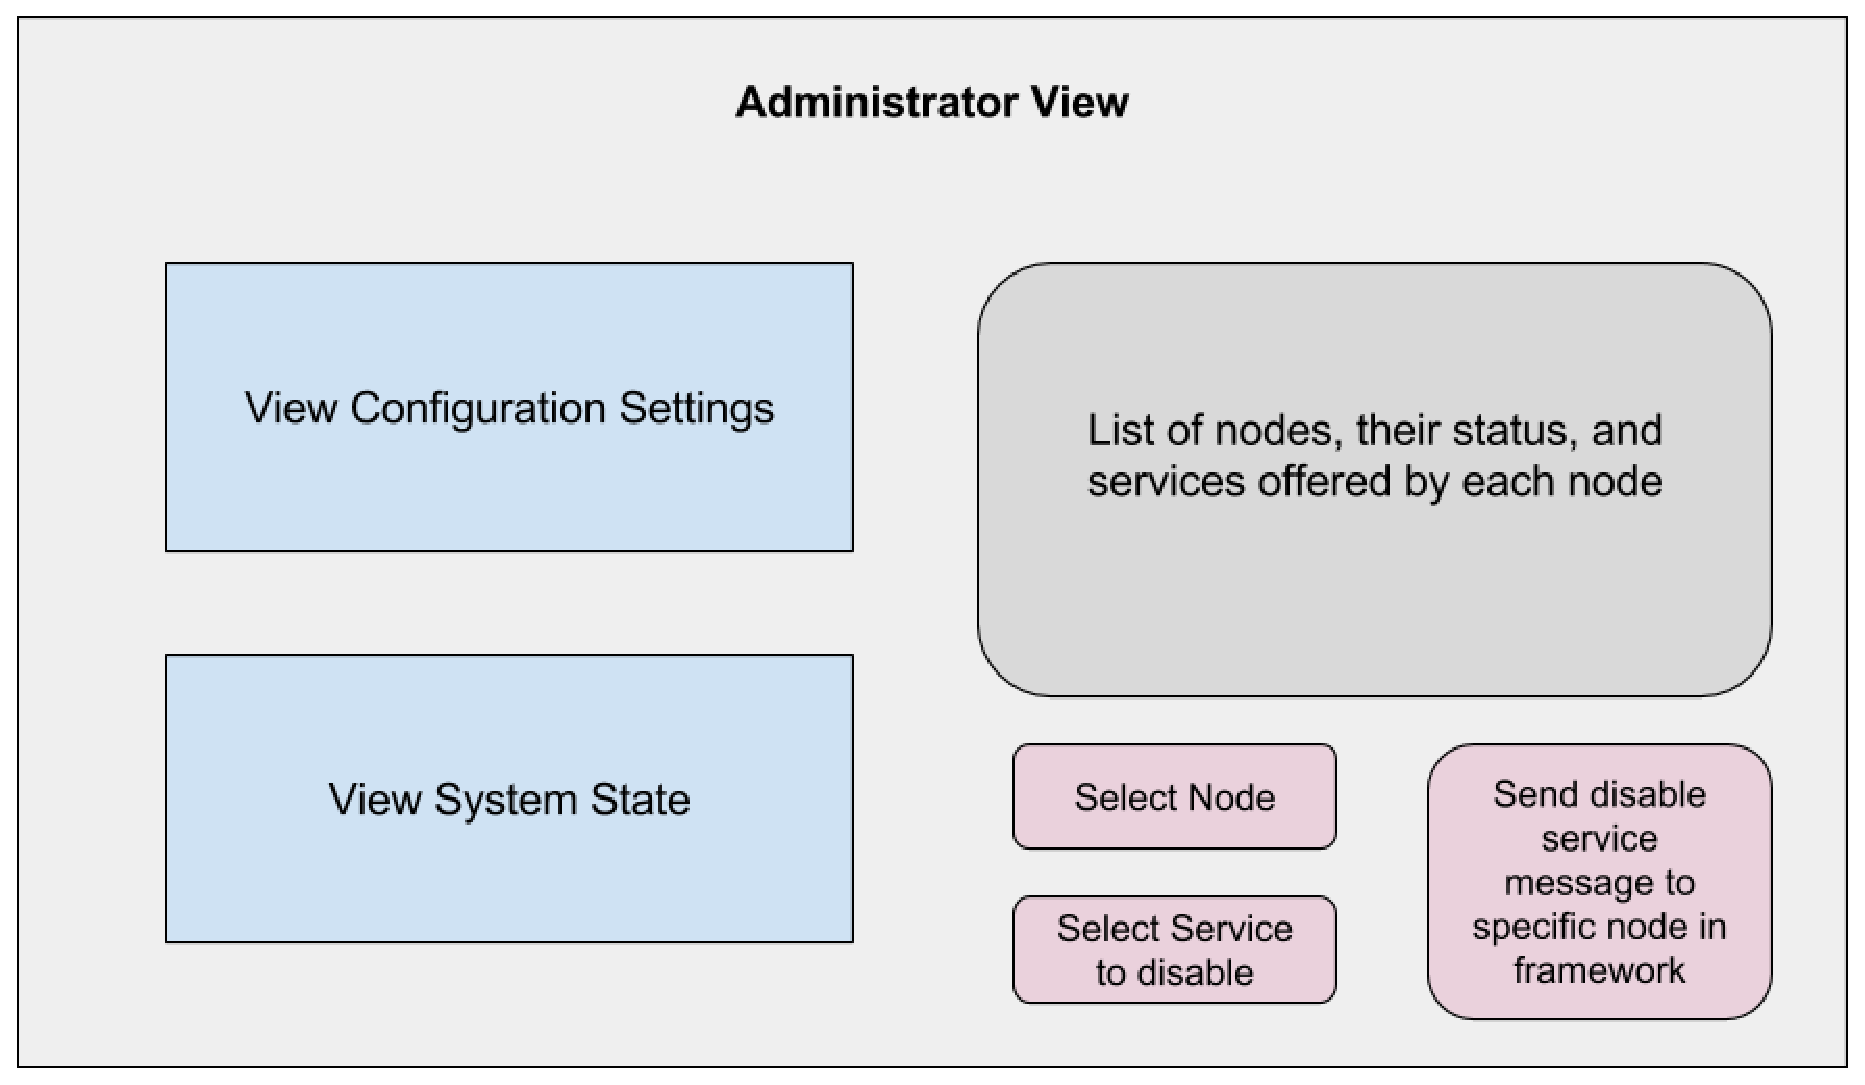
\includegraphics[scale=0.4]{admin}
\captionsetup{justification=centering}
\caption{This figure shows a simple wire frame view of the administrator interface}
\end{figure}




\subsubsection{Summary}
This framework will create a network of loosely coupled nodes that will communicate using a simple messages. It will enable users to input print job objectives into our framework and view the results from a graphical user interface. Nodes will be robust in the face of any mistrusted node. By being a robust framework, it will be able to accomplish objectives without each node having rigid logical configurations. The framework will use a combination of software and hardware. This software will contain core framework functionality, along with the graphical user interface. In the end, this framework will use a combination of software and hardware to enable a collection of wireless, loosely coupled nodes, to self organize on an objective.



%%%%%%%%%%%%%%%%%%%%%%%%%%%%%%%%%%%%%%%%%%%%%%%%%%
\subsubsection{Additions / Changes}
None

\newpage
\section{Technology Review - Hayden}
%%%%%%%%%%%%%%%%%%%%%%%%%%%%%%%%%%%%%%%%%%%%%%%%%%
\subsection{GUI Language}
\subsubsection{Overview}
One part of the ROUS project is user interaction with the system. This is done by creating a Graphical User Interface(GUI). Stakeholders need to be able to see the system graphically and give input, and see some output. Finding a programming language to represent our system to the stakeholders, primarily the user, is going to be a key part of the ROUS project. There are three options of making a graphical interface for the user that make the most sense for this project: using wxPython, creating a web application using ReactJS, or using C\#. These are all very versatile and well-documented portable languages that can create beautiful and user-friendly interfaces.


\subsubsection{Criteria}
The options listed in the overview above need to:
\begin{itemize}
	\item Be relatively easy to use
    \item Integrate well with other languages
    \item Have the ability to create a Single Page Application (SPA)
    \item Be able to create a vibrant colorful and appealing interface
    \item Be easy to test
    \item Take a reasonable amount of time to write in
\end{itemize}
\subsubsection{Potential Choices}
\paragraph{wxPython}
wxPython is a programming language that would help meet the client's needs and possibly allow for further integration in the future because of its parent language Python. Because of wxPython's integration with its parent language, using Python for most of the project would make codependence between the GUI and framework irrelevant. Creating a layout would be simplistic. However, the visual results seem to come out blocky and dull \cite{wxPython}. Portability is another factor to consider. wxPython is fairly portable because it does not take up a lot of space and works on a variety of systems. 
\paragraph{ReactJS}
The second option for presenting our users with a graphical interface is creating a web application primarily using ReactJS. According to Svetlana Gordiyenko at XBSoftware, ReactJs is great for creating Single Page Applications (SPA)\cite{React}, due to the limited space on a microSD card, and increases portability between platforms.
\paragraph{C\#}
C\# is the final option that was considered to be used as a platform to create a GUI for the user experience. C\# is a very well used programming language in the computer science industry. According to the TIOBE index,  C\# has been continuously the third most used programming language \cite{TIOBE}. It is the least forgiving in terms of ease of use. This would add development time in both the development and testing phase. This language also allows for a highly customizable user experience and creative designs. However, doing so takes extra time and testing. One major benefit with C\# is its integration with Microsoft's IDE, Visual Studio. This would significantly decrease the time of development, but would increase set up time and also have less portability.
\subsubsection{Discussion}
ReactJS will be the moderately difficult of the three options. This is because it is less forgiving than wxPython but more forgiving than C\#. C\# will take more time to use in the short span of the project and is more suitable for large scale programs, as opposed to ReactJS, which is more suited for one page applications. wxPython has a very bland interface and seems more like something a developer would use for their personal programs and its needs.
\subsubsection{Conclusion}
After doing thorough research, I have decided to create a web application using ReactJS, because it will be the most portable and beneficial language to write our graphical user interface on. This is because of its portability across different platforms, the ease of use, and its ability to react so dynamically.

\subsection{Threat Introduction}
\subsubsection{Overview}
Another point of interest is how to simulate a threat in the system. Having a threat introduced  will show how the user will be able to both see the effects it has on the system and warn them if their objective can no longer be finished due to the intrusion. Simulating a threat can be difficult as there are many types of “hacks” a Blackhat could use. For the purposes within the scope of the project, there will be a focus on IoT device services no longer being able to work or not working as intended. One option to force a service disruption is by implementing it in the CLI of an individual node. Another option would be to allow the user to simulate a threat by having a button that allows the user to select services of a specific node and disable them. Finally, third option would be to preprogram an objective that faults specific services for a node that they should theoretically be able to do but no longer can, essentially a Trojan type virus. 
\subsubsection{Criteria}
These options need to:
\begin{itemize}
    \item Take short amount of time to take effect
    \item Be able to be visually represented
    \item Be able to change the type of services interrupted
    \item Be easy to test
    \item Take a reasonable amount of time to program
\end{itemize}
\subsubsection{Potential Choices}
\paragraph{CLI}
Creating a command in the CLI would allow easy operation and control by the developer and administrator to simulate a threat within the system. This keeps a user from doing something that they did not know the consequences of. It would also be exponentially faster and require much less fail-safe’s to be programmed. Demoing the project with this feature would require constant attention and access by an administrator.
\paragraph{GUI}
Another viable option would be to create a virtual button within the user accessible graphical interface. This would give more function to the application and a solid foundation for the GUI. This would also require a lot more programming and implementation of fail-safes so the user does not accidentally remove all services from nodes rendering them unusable. However, it would make the demo much more interactive.
\paragraph{Trojan}
The third option would be to create an objective that is essentially a Trojan horse. A Trojan Horse in terms of computer systems is generally defined as "any malicious computer program which misleads users of its true intent. The term is derived from the Ancient Greek story of the deceptive wooden horse that led to the fall of the city of Troy"\cite{Trojan}. This would be accomplished by creating an objective that would be propagated through the system like a normal objective would, but would disable some service. What is great about this method is that it is the most realistic type of threat introduction to a system because this is a real technique a hacker would use. Using a Trojan type of threat introduction would take a good amount of time but would also be the most impressive.
\subsubsection{Discussion}
These three options all are viable. The CLI option would be the easiest to implement. Using a GUI or a Trojan are more difficult, but they would take the same amount of work to produce. The CLI is not the easiest to visually represent to the user. Using the GUI would be the most visually represented. The Trojan can be used as an objective and the user can see the services disappear in real time. Of these choices, the hardest to test would probably be the Trojan.
\subsubsection{Conclusion}
After much consideration and deliberation, creating a changeable Trojan virus like objective seemed to be the best way to simulate a threat. However, this may be somewhat more difficult to implement than other options. It is definitely the most realistic approach and therefore an option that could not be ignored.

\subsection{Testing Framework}
\subsubsection{Overview}
The third point of focus for this project is the testing framework to be used to ensure code quality. Blackbox and whitebox testing are incredibly important for projects of this size. Choosing among these frameworks will help make sure the code is implemented as intended. Creating automated and manual tests for the project is necessary. Of the many different types of testing frameworks, the three most viable options would be: Modular Based Testing, Data Driven Testing, and Hybrid Testing. 
\subsubsection{Criteria}
These options need to:
\begin{itemize}
	\item Have a decent coverage of the code
    \item Be modular
    \item Be scalable
    \item Take a reasonable amount of time to implement
\end{itemize}

\subsubsection{Potential Choices}
\paragraph{Modular Based Testing}
Modular Based Testing is a framework revolved around modularizing different parts of the program. Using this testing method allows for more structured testing and repetition and iterative testing. It will compartmentalize each part of the program which works really well with an agile development cycle. One problem with modular based testing is that not all developers know which parts of the system they are missing and which paths have yet to be covered. Getting full coverage of a program is important in testing and modular testing relies on the developers' knowledge of the system. Modular Based Testing also relies on the programmer to keep track of each piece. Using a modular approach allows the tester to pinpoint exactly where the bug is occurring within the code fairly easily and allows the rest of the code to be untouched.
\paragraph{Data Driven Testing}
The second approach to a testing framework is Data Driven Testing. This method involves a multitude of data to be used within tests to continuously test many options. This works well for programs that require a lot of user input and data manipulation. It is unlikely this will be a good fit for the program because the end product will contain a lot of different data input. To work properly, his method also would require an external database with a lot of fabricated test data. This would involve a lot of prep time and busy-work that could otherwise be used to develop more tests.
\paragraph{Hybrid Testing}
Lastly, a Hybrid Testing framework is a combination of a few different testing frameworks, including the frameworks previously mentioned. It can be modular, data driven, and use a multitude of keywords and test data. This framework would allow for the most coverage of the project. However, it would also require the most brainpower and time devotion. Another downside to this framework is the lack of scalability. Scalability is very helpful in an agile development process because the project starts off small and iteratively becomes larger.
\subsubsection{Discussion}
All of these testing frameworks are valid options. Each would have a good coverage of the code. The Hybrid Testing framework is the least scalable, followed by the Data Driven and then the Modular. Obviously the Modular Testing framework is the most modular of the three options. Compared to the other options, Modular testing would also take the least amount of time to implement.

\subsubsection{Conclusion}
In the end, a modular based testing framework is the most viable option. This method flows better within an agile development process and allows the project to be modularized and automated. If all tests of an agile cycle are not complete, the modular nature of this framework allows some lenience to allow more tests be developed later.\cite{Software_Testing_Help}


%%%%%%%%%%%%%%%%%%%%%%%%%%%%%%%%%%%%%%%%%%%%%%%%%%
\section{Technology Review - Kyle}
%%%%%%%%%%%%%%%%%%%%%%%%%%%%%%%%%%%%%%%%%%%%%%%%%%
\subsection{Problem Description}
To deploy our software system we will need to specify the hardware that it will run on. Developing the software can be done on any system but when it is deployed there are characteristics of a device that would be more ideal then others.  In the sub sections below, I will look at different hardware and contrast the benefits and negatives of each device. In the end I will compare them all and discuss what the best option for the framework is.

\subsection{Arduino Uno}
\subsubsection{Overview}
The Arduino Uno is a low powered open-source micro-controller that has a simple and straightforward development environment. It is great for developing stand-alone devices that control sensors or other hardware. \cite{ada}
\subsubsection{Benefits}
Arduinos are useful in that they are low-powered, cheap, and can do simple quick tasks. They have a robust development environment. There is a lot of information available to help troubleshoot potential problems that we could run into. They have a small form factor which is ideal for deploying our framework. These micro-controllers are ideal for interfacing with other hardware and executing the same task over and over again.
\subsubsection{Negatives}
The issue with using Arduino Uno for this project is that it does not come network ready. You need a separate Ethernet or wireless Ethernet board to enable this on an Arduino. It would add cost and software development time to add this capability. Also, an Arduino is limited to what programing languages can be used for development since it has a rigid development environment that forces a specific language. This device can not run an operating system and has a limited computational capacity. It is also just a micro-controller as opposed to a full computing system. \cite{ada}

\subsection{Raspberry Pi 3 Model B}
\subsubsection{Overview}
A Raspberry Pi is a cheap, low powered, and cost effective replacement for having a full computer. It has all the abilities of a full computer but at a low-powered consumption level. \cite{rpi}
\subsubsection{Benefits}
Raspberry Pis can run an operating system, output video to a screen, output audio, and allow the connection of other peripherals.They have a small form factor that makes it ideal for frameworks like the one we are developing. The Pi can run a full Linux environment which will give us access to any programming language we want to use. By having a full operating system to develop gives us more options and tools to accomplish the tasks. It keeps our options more open and remove the limits of other hardware. Model B has a built in Ethernet and Wireless Ethernet which is necessary for our framework. \cite{rpi}
\subsubsection{Negatives}
An issue with using a Raspberry Pi is that we can find cheaper off brand ones that do the same thing. The problem with doing that is that Raspberry Pis all already low cost and the cost is not an issue to begin with. Another problem with using an off brand on is that there will be less documentation and there will be a greater risk of device failure.
\subsection{Laptop}
\subsubsection{Overview}
I am defining a laptop as a computer that has a modern high speed processor, modern operating system, and built in screen, something that a typical person would consider a laptop.

\subsubsection{Benefits}
The benefits to having a full-fledged laptop would be that would could build and deploy the framework on the same machine. This would give us full network access and a high speed processor. By using a laptop we would have ultimate control over the environment we are in. We could use any operating system or run everything in a virtual machine. There would be no limits on programming languages or other libraries we could leverage to enhance our project. 
\subsubsection{Negatives}
The main issue with a laptop is that for deployment will need more then one device. The cost to have multiple laptops outweighs any benefits it would offer. It would also be a larger form factor then using a smaller micro-controller sized device. A laptop also adds another layer of complexity if we needed to deploy our framework to multiple laptop devices as opposed to deploying to a bunch of the same Raspberry Pis.

\subsection{Comparison}
\subsubsection{Comparison Table}
\FloatBarrier
\begin{table}[H]
\fontsize{3}{4}\selectfont
\centering
\def\arraystretch{1.2}
\resizebox{\textwidth}{!}{
\begin{tabular}{|c|c|c|c|}
\hline
{} & \bf{Arduino Uno} & \bf{Raspberry Pi 3 Model B} & \bf{Laptop}\\ \hline
Power  & 5v & 5v & No constraint \\ \hline
Networking  & None  & Ethernet/Wifi & Ethernet/Wifi \\ \hline
Sensors  & Digital/Analog Pins & GPIO Pins & None \\ \hline
Operating System  & No & Yes & Yes \\ \hline
Cost  & Cheap & Cheap & Expensive \\ \hline
\end{tabular} }
\newline\newline 
\end{table}
\subsubsection{Conclusion}
After exploring the hardware options above, I have concluded that the best option for this project is going to be a Raspberry Pi. An Arduino is not the right pick because it is a straight up micro-controller. It is built to run simple physical tasks on repeat and is not equipped with an Ethernet card. It would cost more to equip each Arduino with the ability to network. This micro-controller is good from projects that do not require a lot of processing. Also the programming language that must be used is limited on an Arduino. You have to program in a specific Arduino IDE that requires the use of AVR C programming language. This is limiting and it is not necessary to limit ourselves to one language.
\\ \\
Having a full fledged laptop would be over kill for our deployment of the framework as well. It would not be cost effective and would require a lot more setup. Also a laptops larger form factor would be cumbersome for the deployment of the framework.
\\ \\
In the end the best option is going to be a Raspberry Pi. This device is low powered and cost effective. It comes equipped with Ethernet capabilities and a large amount of processing power compared to an Arduino. This device can run a full Linux environment which would not limit us to a specific programming language and give us more options all around in terms of design. The Raspberry Pi will give us a solid foundation in which to deploy our framework on.


\subsection{Network Protocols}
\subsection{Problem Description}
The framework will need to have the ability to communicate with nodes in order to share resources. This communication needs to happen across physical distances using standard Internet protocols. Below the sub sections discuss the benefits of different network transport protocols we could use to solve this problem.
\subsection{TCP}
\subsubsection{Overview}
TCP is a connection-oriented transport protocol that sends data as an unstructured stream of bytes.\cite{Cisco} This protocol information about packets transmitted to a destination node by using sequence numbers and acknowledgment messages. Loss data is retransmitted by TCP until all data has been retrieve successful or a timeout occurs. It can determine if a duplicate message has been sent and trash them. In this protocol there are mechanisms to control the flow of data and communicate with other layers to convey information. \cite{Cisco}

\subsubsection{Benefits and Negatives}
The main benefit to using TCP is that is reliable. We would be able to trust that every packet sent was sent correctly and error free. In our framework we will have to transfer files, using TCP would ensure that the files we transfer are not corrupted. 
\\ \\
A negative to using TCP is that we wont be able to multi cast. Being able to broadcast a message to multiple devices at once would be a benefit for our framework but TCP would not allow us to do that. Also TCP uses more bandwidth then other protocols which would be a negative to our framework if latency was an issue.

\subsection{UDP}
\subsubsection{Overview}
UDP is a connectionless transport layer protocol that provides a basic and unreliable message service to interact between the IP and upper layers.\cite{kits} This protocol is capable of can identify by port the different applications running on a single device. UDP is not reliable in that is does not ensure that every byte of data will reach its destination. It contains no flow control or error recover but is has less network overhead. This is due to the protocol not having to make sure that every packet was received. All that error checking adds overhead which UDP does not have to deal with. \cite{kits}

\subsubsection{Benefits and Negatives}
Our framework would benefit from the lower network overhead that the UDP network protocol offers. UDP allows multi cast which would give our framework the ability to broadcast messages to multiple nodes at once. This ability would enhance our framework. The issue with using UDP for our framework is the unreliable data transfer. Our framework requires us to transfer data uncorrupted and by using UDP we would have no ability to ensure data was sent and received error free.

\subsection{SCTP}
\subsubsection{Overview}
SCTP is a not well known transport layer protocol. It is similar to TCP in that it is reliable, confirming that data is received in order and with no errors. This protocol is message oriented like UDP and not byte oriented like TCP. Unlike TCP this protocol is session oriented and ensures a relationship between only two endpoints before data is sent, this adds an extra layer of security to this protocol. The main difference that SCTP was trying to achieve over TCP is removing some of the limitations that TCP has. \cite{realtime}

\subsubsection{Benefits and Negatives}
The benefits and negatives of SCTP are similar to the benefits and negatives of TCP. SCTP only added benefits over just using TCP is its added security. But there are not requirements for having extra security over what any of the other more known protocols offer.

\subsection{Comparison}
\subsubsection{Comparison Table}
\FloatBarrier
\begin{table}[H]
\fontsize{3}{4}\selectfont
\centering
\def\arraystretch{1.2}
\resizebox{\textwidth}{!}{
\begin{tabular}{|c|c|c|c|}
\hline
{} & \bf{TCP/IP} & \bf{UDP} & \bf{SCTP}\\ \hline
Reliable  & Yes & No & Yes \\ \hline
Transmission & Bytes  & Message & Message \\ \hline
Security & Yes & Yes & Yes \\ \hline
Data  & Strictly Ordered & Not Ordered & Partially Ordered \\ \hline
Connection  & Specified & Connectionless & Specified \\ \hline
\end{tabular} }
\newline\newline 
\end{table}
\subsubsection{Conclusion}
All of the above network protocols all have their advantages and disadvantages. TCP is useful because it is reliable and ensures data is correct and error free. UDP is also useful because it has a lower overhead and is best in situations where reliability is not needed. Lastly SCTP helps to fix some of the limitations with TCP but it is not as known and would not add any extra benefits for our framework over just using TCP.
\\ \\
This framework will require that all data is transported successfully without error. It does not require fast transmission rate or have limits on bandwidth. UDP does not satisfy the requirements of what our framework will need and thus is not a good choice. SCTP will also not make a good choice because it is not as wide spread and has no benefits over TCP when it comes to this framework. 
\\ \\
It seems that TCP would be the best choice when it comes to network communication protocols for our framework. The protocol allows for a reliable connection that will ensure that all packets are successful and error free. In the end TCP is suited for the needs of our framework.



\subsection{Parallel Programming Models}
\subsection{Problem Description}
The software framework that we are building needs allow the sharing of resources and processes. One way we could allow this sharing is through parallel programming. In the sub sections below I will discuss the different models of parallel programming, how they compare to each other, and which one might be most suited for our framework.

\subsection{Shared Memory}
\subsubsection{Overview}
There are two different implementations of a shared memory parallel programming model. In the non-threaded model processes and tasks read and write asynchronously to common address space. Semaphores are a must in a non-threaded shared memory model in order to prevent race conditions and deadlocks. \cite{PP}
\\ \\
The other implementation of a shared memory parallel programming model is the threaded model. This model has a single process that contains more then one concurrent execution path. For this framework I will be focusing on the threaded model of the shared memory parallel programming model. \cite{PP}
\subsubsection{Benefits and Implementations}
The benefits of using a threaded shared memory model is that each concurrent thread will share the resources of the "master" process. All threads share a global memory. This helps us solve the problem of our framework needing to share resources. Each thread will also have its own local data. \cite{PP}
\\ \\
There are two standardized implementations of the shared memory parallel programming model, POSIX Threads and OpenMP. The POSIX thread model is a c language implementation integrated into Unix operating systems, it is very explicit parallelism. OpenMP is a portable and multi-platform model that can be used on a wider variety of systems. Instead of explicit parallelism, OpenMP provides incremental parallelism. Our framework would benefit more from the OpenMP shared memory parallel programming model because of its portable and multi-platform model that allows it to be used on a wider variety of systems. \cite{PP}

\subsection{Message Passing}
\subsubsection{Overview}
In the message passing model, there is a set of tasks that have their own computation memory. These multiple tasks can be located on the same physical device or spread across multiple devices. The tasks just the sending and receiving of messages as a way to communicate. This transferring of data requires each tasks process to cooperative in order to share data, thus a send must always have a receive. \cite{PP}
\subsubsection{Benefits and Implementations}
The message passing model has only a few benefits for our framework. Since it is a parallel programming model it will allow the sharing of resources and contains built in structures for the sending and receiving of data. Another benefit is that this model has been packaged into a standardized form call MPI. This MPI platform is available for a wide variety of systems and portable to lots of devices. \cite{PP}

\subsection{Data Parallel}
\subsubsection{Overview}
This model is also refereed to as the Partitioned Global Address Space (PGAS) model.\cite{PP} In this model the address space is global and most of the parallel work focuses on doing operations on a data set. Data parallel has tasks that work collectively on the same data structure but each task is assigned to a different partition of that global data structure. \cite{PP}
\subsubsection{Benefits and Implementations}
This model does not offer any benefits for our framework. It is mainly used to run operations on large data sets. More commonly used implementations of this model are written in Fortran. Most implementations are in the developmental phase and would require a lot of research just to get up and running with them. \cite{PP}

\subsection{Comparison}
\subsubsection{Conclusion}
After exploring the parallel programming models above it became clear to me which would be the best option for our framework. The shared parallel programming model offers the most benefits to the implementation of our framework. Its threaded model fits the needs of our framework to share resources. This OpenMP library that implements the threaded shared memory parallel programming model is wide spread and available on variety of hardware. Since this library is more wide spread and it has more support and documentation which would ease in the development. The OpenMP would give us more options and not limits us. In the end the best option for parallel programming models is the shared parallel programming model using the OpenMP library.


%%%%%%%%%%%%%%%%%%%%%%%%%%%%%%%%%%%%%%%%%%%%%%%%%%

\newpage
\section{Weekly Blog Posts}

\subsection{Hayden}
\subsubsection{Fall}
\paragraph{Week 1}
This week was spent deciding what projects I would like to work on for capstone.I created a list of all of the ones that seemed interesting to me. For my final five, I chose what interested me the most as well as some consideration to the companies I would like to work with. I really like IoT because to me, it is an emerging market and I would love to get in on the growth of IoT and maybe even help shape what it becomes. 
\paragraph{Week 2}
This week I found who was in my group after a long weekend of worrying. I got my number one choice working on the Internet of Things collaboration project for HP.  We met our client Lonnie Mandigo and decided to focus on a security portion of Internet of Things and how to mitigate a security break-in with a mesh nodal structure.  We also found that we won't have to create any middle-ware onto any existing device but rather use arduinos or raspberry pi's to be the middle man and IoT connectors. We also settled on using Scrum as our development process and settled on Mondays at 4:30 to do our weekly sprint review meetings via Skype.  We also settled on a name for our project, Collaborating Threat Mitigation, or CTM for short.  And we reserved a study room in the library for the meetings. Lonnie also decided that I will be the one to take project ownership which is an amazing opportunity, but also a LOT of responsibility. I think I'm up for the task though. 
\paragraph{Week 3}
This week we narrowed down more of what we are going to work on for our project and some specific features we want to focus on. We also met with our TA and set up weekly times for our TA meetings. 
\paragraph{Week 4}
This week we decided to change our weekly review scrum meetings on Tuesdays at 4 to give us more time to discuss the project. I think we are going to use raspberry pi zeros as nodes.   
\paragraph{Week 5}
This week we finished up a little more fine tuning on the problem statement and made sure we were all on the same page. We finished our rough draft of the requirements document, but there is still plenty of editing and adding we need to finish before our final draft. We had a good weekly review meeting on Thursday with Lonnie.
\paragraph{Week 6}
This week I had a meeting with our client, Lonnie, on Monday to get some feedback on our requirements document and gave him a copy of it.  
Tuesday we worked a little on the requirements document and also had our weekly review with Lonnie.  

The rest of the week, Kyle and I made changes and modifications to our requirements document. We sent an updated version of our requirements document to Lonnie on Wednesday.
\paragraph{Week 7}
This week we decided which parts we wanted to write about for the tech review. I am in charge of the UI portion and getting input from users as well as the start of the threat. Another main portion is how we are presenting the user with a visual of how the results are being shown. I need to find a good representation of how to our system so that a user can understand what's going on. Most of what I am working is the high level directly with user input and output to the user.  
\paragraph{Week 8}
This week, Kyle and I got to really start focusing on the design portion of the project. We made an appointment with Lonnie to meet on Monday and flesh out a lot of the design for our project and how we are doing it. We decided that creating a threat would be really good to act as if it is an objective for the system. The system will do the objective which would be disabling some service on a node or two. The following objective will have to make it through the system and complete successfully. We also decided on doing a web app using ReactJS so that anyone that is connected to the self-sustained network can connect to the nodes and we might need to create a sign in to have authorized users to see it. The GUI is going to most likely be a Single Page Application.
\paragraph{Week 9}
This week I finished up my tech review and had a great meeting to talk about design with Lonnie and Kyle. We decided to create a system that bids on services of an objective if the node can do the objective. Each will broadcast a random number and compare their number to the numbers received from broadcasts. If there are no numbers higher than their broadcasted number, once the bidding phase is over, it starts the job. I also started the design document and tried to get as much of it done as I could. 
\paragraph{Week 10}
This week we worked more on the design document. We got our first draft together and completed it by Tuesday. We sent it out to our client, Lonnie, by Wednesday. He gave us some tremendous feedback the following day and we have been working on implementing that since. I also started the progress report and I am a little nervous I will not get it done in time, but I think I will. 
\subsubsection{Winter Break}
\paragraph{Break Notes}
Over break I got the Raspberry Pi's I borrowed from Kevin and received one of my own for Christmas. I spent some time figuring out what I needed to make the Raspberry Pi's work and how to connect to them headless without ever having to connect a monitor to them. I started making some random sketches for how I envisioned the user GUI.
\subsubsection{Winter}
\paragraph{Week 1}
This week we started our weekly meetings with Lonnie again. We decided on a finalized starting version of our product. A simple program allowing our raspberry Pi's to be on the same network and talk to each other. 
\paragraph{Week 2}
This week Kyle and I got a good core portion of the project done. I found ways to make the onboard LED's of the Raspberry Pi's to turn off and on and blink how I pleased. We have a simple messaging system between nodes available and each have their own IP address. 
\paragraph{Week 3}
This week we got the bidding done other than some slight timing issues done, and I started a GUI. We had a meeting with Lonnie in person on Thursday and showed him a demo of the Raspberry Pi's and where we are at. 
\paragraph{Week 4}
This week we talked over having a queue and why that would be a bad idea. Having a queue isn't necessary and almost always will lead us into having state-full exchanges. And we want to keep the system stateless. 
\paragraph{Week 5}
This week I worked on creating a web server out of the Raspberry Pi's and a GUI that will allow us to have a friendly interface that anyone can use as opposed to the command line. I started off using an Apache server and decided to switch that for a node.js server. Then I created a react-web-app and integrated my react web-app with Bootswatch for a quicker and better looking theme. We also met with our TA Andrew, he said we were ahead of the curve on how far we have come. Our client, Lonnie, also seems to be happy with how far we have come and where we are currently at with the project.
\paragraph{Week 6}
This week I spent my most of my time working on the css to try and get the formatting looking halfway decent. I also spent a good amount of time figuring out what the base dependencies would be needed for my app to still run correctly. By doing this, I found there to be a lot of "fluff" that was downloaded but not actually needed within the react-app. 
\paragraph{Week 7}
This week I started off continuing with my react-app and adding functionality but it was pretty slow going due to the amount of work needed for formatting. About half way through the week, Kyle, showed me some stuff he had been working on with Bootswatch, an add-on that automatically formats things for you fairly decently. With this new information and work, I switched full time to using codesandbox.io and using Bootswatch for my formatting. This made the work much more efficient and quicker. 
\paragraph{Week 8}
This week while working in codesandbox.io, a web IDE, I got a lot of components done for the administrator page. I also took some time to learn about statefulness within react and how to mount and unmount components. This change started to make the website much more dynamic and change depending on different inputs. I wasn't sure how the backend was going to send the information I needed to dynamically change events on the screen, so I was using manual input for the dynamic elements until we figured out how to format the information that was coming in from the server.
\paragraph{Week 9}
This was a really busy week. A lot of the time spent was changing how to the frontend was doing the GET requests and changing from using a library called AXIOS to using Fetch. Both of which use AJAX to make their server calls. I was now able to query the server but still wasn't sure what format I would be getting the information in. I changed it to accept the way we currently thought it was going to receive information. A simple JSON object.  
\paragraph{Week 10}
This week I was absent due to Intercollegiate Racquetball Nationals with my team. In terms of the project I really just reminded everyone involved that I would be off the grid and would be available again on Monday 3/19. It was a long week in Minneapolis, Minnesota. I ended up placing third in my division and our team took first in overall team. Both the men's and women's team placed second. It was a long and tiring week but a nice break from schooling.  When I got home from nationals, I found Kyle had taken some time to work on the GUI and made a new front end and made the back end talk together very nicely as well as added a button to mistrust current nodes. He also found out that using AJAX would cause a delay of about 20 seconds when talking with the server and the front end so we resorted to using socketio operations from the front end instead. 

\subsubsection{Spring}
\paragraph{Week 1}
Over spring break I spent a good amount of time trying to figure out the changes Kyle made to the front and how we could change it to make it work better. I spent the majority of the time trying to get it to work and find the new dependencies needed. This week I got it to finally work and am now trying to figure out how the front end works after Kyle's rework and how to get the styles how we want them to with the current setup. Another good amount of time was spent trying to find a good meet up time with Kyle to work on the project and when we should have our TA meetings as well as our meetings with our client. We settled on Wednesdays at 4pm for our meeting with Lonnie and still have not heard back from Andrew yet.
\paragraph{Week 2}
Throughout the week i worked on getting the printing service to actually send the contents of a file through so the printer would print what the user wanted to print. It works by the user picking the file they want. Then grabbing the contents of that file and adding it the end of the print service JSON message. The node that wins would save this text to a local file and then continue on printing how we had before. I got some feedback from Kyle which was great. This weekend I plan on changing it to actually send the entire file over and not just the contents so we have more range with what we can do.
\paragraph{Week 3}
On Tuesday I gave an update on the system with Lonnie and confirmed some specific things he is looking for in the demo he wanted. Later in the day, I found out Kyle was in the hospital. I'm glad he's okay. I spent a lot of this week fixing some GUI issues and trying to get the printing to send the file correctly. 
\paragraph{Week 4}
This week we tried to get a demo done, but Kyle really wanted to make sure it was perfect and ready for Lonnie and HP. We met with our client, Lonnie, in person and were able to get more insights on what he's looking for with the demo. This week I also fixed a bug we were having in the GUI where the console log was spitting out multiple IP addresses that were blank.  
\paragraph{Week 5}
This week we made a demo for our client on Tuesday that he wanted by Wednesday. Unfortunately, the sound on the demo dipped out, so Kyle remade the demo other than a couple slides I was talking in. Because of this, we knew we had to make another demo. We met with our client remotely on Wednesday and got some good feedback. We changed things with the demo and made a new one today, Friday (5/5). This demo went a lot better and we are definitely more proud of it. This week I made more services in the configuration file and services file. Kyle fixed his block graph and fixed the multi message data coming in to the log.  
\paragraph{Week 6}
This week I tried to figure out a way to show current state. This proved to be hard in a stateless system. I worked on different prototypes with current code to see what would work best for expo. We talked with Lonnie on Thursday and learned the value of taking a step back and comparing risk and reward. This put the amount of time spent on the graph into perspective.  
\paragraph{Week 7}

Expo week, this week we tried to just make the GUI a little more user friendly for demoing it off during expo. Kyle pushed new code to master the night before expo. The new code helped with the timeline on the graph be a little more understandable but broke the trusting node functionality.
\paragraph{Week 8}
I took the week off of project work, but we did meet with our client on Thursday night to talk about possible future uses of the ROUS framework. One of Lonnie's only complaints about our project was showing an incomplete product at expo and showing a product that had more features but was less stable. We also set up a demo time to demo our system at HP. We set this demo up on the HP campus on Friday June 1st. I'm excited for it! 
\paragraph{Week 9}
This week I tried to make the system usable with my set up again. There were a lot of static changes made to be specific for the expo demo setup. We met with Lonnie's luncheon IoT group and presented our project to HP employees.
\paragraph{Week 10}
This week we made a couple of changes to our midterm progress report and used it as our final presentation because it already followed the correct format. I also started the final report and got all of our original documents included and formatted into the final report. 


%%%%%%%%%%%%%%%%%%%%%%%%%%%%%%%%%%%%%%%%%%%%%%%%%%

\subsection{Kyle}
\subsubsection{Fall}
\paragraph{Week 1}
This week I read and thought about what projects that I wanted to work on. I bid on the projects that I thought were interesting before the assigned deadline. Then throughout the week I researched different ideas related to the projects that I had bid on. 
\paragraph{Week 2}
This was an exciting week for everyone! 

On Tuesday we were assigned to our project and learned who our group members were. Group members meet each other for the first time, exchanged contact information, and discussed their initial impressions of how they saw the project working. Slack was created and each team member shared their individual OneNote with the other members of the team. 

Wednesday we contacted our client for the first time. We heard back from Lonnie(client) that same day. Our first client meeting was set up for the next day. We scheduled to have lunch at Mcmenamins. 

Thursday was our first client meeting. This was a lunch meeting at Mcmenamins on Monroe. The meeting was productive and a more specific use case for the project was decided on. It was great to meet Lonnie and exciting to get started on this project. 

The rest of the week and through the weekend was filled with more discussion among team members on Slack. We discussed and voted on a group name. The group github and blog were created. 
\paragraph{Week 3}
Productive week! Our team started off the week by finalizing our group project name!  This week our problem statement rough drafts were due. We were required to bring a copy to class and get advice from fellow students. A project github was created. 

On Wednesday the group had their first meeting with the assigned TA, Andrew. He outlined what his role is and what he requires from us. We will have weekly meetings with Andrew. Further discussion of the project continues on Slack.  
\paragraph{Week 4}
This week we have to finalize our group problem statement and send it to our client by Friday. Our client will need to verify that they received a copy of our problem statement. 

On Tuesday we had a productive team meeting. We shared ideas about how we see the project working and what the requirements document might look like. We ran into an issue with Skype and were unable to have a conversion with our client Lonnie. It was a frustrating experience but discovered that it was Skype who was having issues, causing us not to be able to login and having sound issues. Due to these issues Lonnie was kind enough to reschedule for Thursday. 

Thursday we had a productive team meeting. Lonnie skyped in. We discussed our problem statement and how to improve it. We went over different topics related to further narrow down our specific user stories that we will be working towards.  We started discussion on the requirements document. 

Lonnie introduced a good tool for framing a problem SCIPAB https://www.linkedin.com/pulse/20140801190140-4204130-scipab-the-six-step-method-for-starting-important-conversations-and-presentations 

Friday we got the privilege of getting to go to a lunch meeting on HP campus. Lonnie invited us to a weekly informal lunch meeting where he and his colleagues discuss different topics related to IoT devices and technologies.   

We were able to introduce our problem to the group and get their insights and feedback. It was enjoyable to listen to people much smarter and more experience on their take on the project. People always have a good way of thinking about project in different lights. 

After the lunch meeting we got a tour of the HP campus. Very big campus. We got to check out their massive printers and the cool spaces they get to hang out.  

Once we finished the meeting we all grouped up in Lonnie's office to discuss the project. We discussed the development of our user stories. Lonnie made very helpful and insightful comments. He has helped to further focus us on a specific use case and goal. It was a very productive meeting and a really fun afternoon.  
\paragraph{Week 5}
The goal for this week was to produce a rough draft of the requirements document using the IEEE standard as a guide. On Tuesday we did not have our regular client meeting and had it rescheduled for Thursday. The team meeting on Thursday we had a great feedback from Lonnie on different sections of the requirements document. We were able to get input and here his thoughts and ideas on how we are moving forward with the requirements document. 
\paragraph{Week 6}
This was a very busy week. All week Hayden and I worked on the requirements document. Lots of work done improving the document, adding images, and reducing the "fluff". Tuesday we had a team meeting with the TA and a team Skype meeting with Lonnie. At the Skype meeting Lonnie helped us to remove some of the "design" out of the document.  

Team name and Project name have changed. Project ROUS is the project name with the team name being Rodents of Unusual Size(ROUS). Lots of work all week on the requirements document. 
\paragraph{Week 7}
Finished finalizing the requirements document and getting it approved by Lonnie and approval email sent out to professors. 

This was a stressful week when it comes to group dynamic issues. Other than that it was a productive week on my individual technology review document. I have my document laid out and all technology's picked. I am finishing the research on my last section and finishing up the document before I got back though and correct errors. 

All and all it was a stressful but productive week. 
\paragraph{Week 8}
Tuesday the rough draft of the tech document was due. We reviewed documents in class and got feedback from another student, this was a graded exercise.  

Thursday we had meeting with client. We discussed design document and Lonnie gave lots of advice. Wanted us to check out resin.io. 

Monday we have an in-person client meeting with Lonnie to go over design stuff. 
\paragraph{Week 9}
This week started out really productive and ended with Thanksgiving, was a good week. Hayden and I had an in person "work" meeting with Lonnie. Lonnie came to OSU and we had a two hour open discussion about the design of our framework. It was a really productive meeting. He helped answer questions. After the meeting it made it a lot easier for us to dive into the design doc. 

The rest of the week was just spent working on the design doc. Thursday was Thanksgiving and not much work happened on that day. Friday was spent recovering from Thanksgiving. All in all it was a good productive week, and we had a really good meeting with Lonnie
\paragraph{Week 10}
Good last week of the term. Had a productive meeting with Lonnie where he gave us really amazing feedback on the Design Document. This feedback helped to improve the document.  

Hayden and I spent the first part of the week finishing up the first draft of the document. On Wednesday we sent the document to Lonnie and he gave us hand written feedback. Then on Thursday during our Skype meeting with Lonnie we got to clarify some questions we had and get more quality feedback from Lonnie. 

Friday was sent making changing and cleaning up the different sections that were still not correct. After polishing the document up, I submitted it to GitHub and the OneNote
\subsubsection{Winter}
\paragraph{Week 1}
Good start to the term. It is nice that we do not have class every day this term. 
Meet up with Hayden and discussed progress and moving forward this term.  
Meet with client and had a good conversation. We talked about the current progress made and what we are doing next. We discussed what the term as a whole looked like and then went into what the next couple weeks look like. 
\paragraph{Week 2}
\begin{lstlisting}
commit 054d2256fa1122d44cf880d2e401da583c4d536a 
Author: kyle <kyle@prouty.io> 
Date: Wed Jan 17 20:52:58 2018 -0800 

small refactor. added gitignore 

commit ff00b2caec7be029d86bcb850445679917a91042 
Author: kyle <kyle@prouty.io> 
Date: Wed Jan 17 20:39:45 2018 -0800 

getting the code that I lost remade. Going well. Got project structure mostly set back 
up. Redoing features 

commit 720714b40da32adb1e59ccc9e09fa7526f2ac6a5 
Author: kyle <kyle@prouty.io> 
Date: Wed Jan 17 16:05:56 2018 -0800 

Setting up code structure. Rewritting lost code that was lost due to hard drive failure. Initial node server is working. Working on Services functions 

commit bbae74e383ca5ff70cf024f8a891b58bdda20dc3 
Author: kyle <kyle@prouty.io> 
Date: Thu Jan 18 22:06:34 2018 -0800 

small refactor and rename 

commit eb2fd02feca5269475254daec0a5bf89e803a926 
Author: kyle <kyle@prouty.io> 
Date: Thu Jan 18 20:11:56 2018 -0800 

fixed annoying thing were you couldn’t ctrl-c to shut server down12 

commit dfe2890f34b27ab3917b4b320f6390b3f231b8de 
Author: kyle <kyle@prouty.io> 
Date: Thu Jan 18 17:04:22 2018 -0800 

Working on services, working on user, basic functionality basically done 

commit 324d682d2b83d3aeb3bbdffa538952f28dc92a8e 
Author: kyle <kyle@prouty.io> 
Date: Fri Jan 19 15:13:35 2018 -0800 

got auto-finding local IP working, finishing auto-whitelist of nodes 

commit f9bceb458f1aeae101f931d1091ad22caef97796 
Author: kyle <kyle@prouty.io> 
Date: Fri Jan 19 10:54:34 2018 -0800 

cleaned up node discovery code, split it up into more functions 

commit b487639616eb07acc551ce8aa163e705c7da4645 
Author: kyle <kyle@prouty.io> 
Date: Fri Jan 19 01:49:54 2018 -0800 

node discover working, parsing IPs working, updating whitelist working. Have basic logic 
now for any new node discovery 

commit 257f855c8944e1d1cecb8e6b5de8ec767931a67b 
Author: kyle <kyle@prouty.io> 
Date: Fri Jan 19 01:15:20 2018 -0800 

got node discover function working in utils, working on auto whitelist 
\end{lstlisting}
\paragraph{Week 3}
\begin{lstlisting}
commit c6ef18939dbabf39d5b1587030f1e8da9383ebbe 
Author: kyle <kyle@prouty.io> 
Date: Mon Jan 22 16:48:49 2018 -0800 

working on user interface. auto generating host list. also setting up more leds, adding them to services. next is to finish the bidding 

commit cccc6c46e265461b8d53c5848bd092edafb520b7 
Author: kyle <kyle@prouty.io> 
Date: Sun Jan 21 01:53:49 2018 -0800 

threads working corretly to manage LEDs. User can turn LEDs on and off of nodes. working on bidding next 

commit 2fd280be1fd3eb999af9876371a4069159e7d06d 
Author: kyle <kyle@prouty.io> 
Date: Sun Jan 21 00:39:03 2018 -0800 

fixed LED issue by making the LED logic run in threads. Cleaning up this code now 

commit 9aeaddb9cb4715282fe0f81e9beece72a251266a 
Author: kyle <kyle@prouty.io> 
Date: Sat Jan 20 21:08:11 2018 -0800 

implemented more services logic to turn on and off leds on Rpi, kinda broken still. Working on implmenting more user stuff. Working on outputing logs to admin. 

commit 02091b25a635b6968bc82e63f0106b4f63118670 
Author: kyle <kyle@prouty.io> 
Date: Wed Jan 24 14:19:30 2018 -0800 

refactored code and added network module in utils, fixed a few bugs, working on bidding and file transfer 

commit aea31a4085afcd6fa2a0674e6d6b42174a751d16 
Author: kyle <kyle@prouty.io>11 
Date: Wed Jan 24 14:16:46 2018 -0800 

refactored code and added network module in utils, fixed a few bugs, working on bidding and file transfer 

commit 7f3ec96243b15ff8dac781212752a0ba054eee8e 
Author: kyle <kyle@prouty.io> 
Date: Thu Jan 25 23:17:58 2018 -0800 

bidding working but having issues with LEDs and threads. On the right path but demo didnt happen. 

commit c0940a0b1c4a5246bb5b4c97b755e6877cef77d6 
Author: kyle <kyle@prouty.io> 
Date: Thu Jan 25 17:40:53 2018 -0800 

multicast message sending working well. Initial bidding working, still testing. 

commit 95f927f0508f5fcfe98bb68df1cdf2aeadd4625a 
Author: kyle <kyle@prouty.io> 
Date: Thu Jan 25 16:37:24 2018 -0800 

refactored network communication to use multicast instead of unicast. 

commit 67404f465cd9604691b22083792915cc869d4bc8 
Author: kyle <kyle@prouty.io> 
Date: Fri Jan 26 23:25:33 2018 -0800 

fixed bidding, working on fixing led thread stuff, its not working how it should 
\end{lstlisting}
\paragraph{Week 4}
\begin{lstlisting}
commit f3f24811ddacf8277878e1420f05a338e3badfa0 
Author: kyle <kyle@prouty.io> 
Date: Fri Feb 2 23:18:31 2018 -0800 

still tweaking bidding. problem is with recvfrom since data size is unknown and recvfrom always blocks. I think I have it fixed and stable but I am still looking for bugs 

commit 6f904d3dfb40a24edc40a3298abf394079df4f45 
Merge: 532662c f469b33 
Author: kyle <kyle@prouty.io> 
Date: Fri Feb 2 22:27:33 2018 -0800 

Merge branch ’master’ of https://github.com/RodentsOfUnusualSize/RodentsOfUnusualSize 

commit 532662c0123c809c97f6ecd46bed3b49bf2a7621 
Author: kyle <kyle@prouty.io> 
Date: Fri Feb 2 22:26:44 2018 -0800 

fixed bidding, it is working correctly now. Still testing and looking for bugs. Started on adding more functionality 
\end{lstlisting}
\paragraph{Week 5}
\begin{lstlisting}
Busy week for me in other classes due to midterms. Worked on bugs. Had a client meeting that went well. Talked about what we are working on and what problems have come up. 
\end{lstlisting}
\paragraph{Week 6}
\begin{lstlisting}
Overall this was a busy week but productive. We got an initial draft done of our poster. Later in the week we had a productive meeting with Lonnie and got some good feedback on some issues I was having with the logic and features I wanted to implement.  
Hayden and I recorded our video presentation and finish the write up report that went along with it. I signed us up to do a peer poster review with another capstone team. 

commit 188345f9994a7558578f507fcac411a3ad85945b 
Merge: 2677b74 a76a150 
Author: kyle <kyle@prouty.io> 
Date: Fri Feb 16 23:44:03 2018 -0800 

Merge branch ’master’ of https://github.com/RodentsOfUnusualSize/RodentsOfUnusualSize 

commit 2677b74b4bbf9945a615fa896eaaae8bc24bcb32 
Author: kyle <kyle@prouty.io> 
Date: Fri Feb 16 23:43:36 2018 -0800 

mid-term progress report 

commit a76a150ba0d2bce427f56f5745107354a585438b 
Author: proutyio <kyle@prouty.io> 
Date: Fri Feb 16 11:06:49 2018 -0800 

Update .gitignore 

commit d1825cb100b2d81b625b9ba5c450f87fe52dd8b8 
Author: kyle <kyle@prouty.io> 
Date: Fri Feb 16 09:18:33 2018 -0800 

removed unneeded files. added nodesmodules to gitignore10 

commit 4ec003e6d43c6f0ae26c5e41ed02ef1115b20918 
Author: kyle <kyle@prouty.io> 
Date: Fri Feb 16 09:15:26 2018 -0800 

removed unneeded files. added nodes modules to gitignore 

commit 2b75a30173526e4b7062a7e2b9f1727556603b50 
Author: kyle <kyle@prouty.io> 
Date: Sat Feb 3 00:05:01 2018 -0800 

bidding stable now. need to clean up code now, look for edge cases 
\end{lstlisting}
\paragraph{Week 7}
\begin{lstlisting}
Busy week.  Tuesday everyone in class had to meet and we had a guest speaker. I really enjoyed the lecture and it was a good class. I made progress on different parts of the code this week and improved some of the bidding. Thursday our group had to go to a class meeting with ten other groups. We talked about what is coming up this term and answered questions about posters and expo. Wednesday we had an in person meeting with Lonnie. The demo didn’t work out and we ended up going out for some drinks and food. All and all it worked out. I got cfg stuff done and nodejs server with react frontend that can listen for multicast messages from the nodes. 

Got some bugs worked out. Got a solid configuration setup implemented that helps add a lot of functionality and will help to expand services. Also got a nodejs server implemented that runs a react frontend. Make file loads both backend and frontend. Nodejs server also runs a multicast listener that listens for any messages sent out from the nodes. Lots of good logic done. 
\end{lstlisting}
\paragraph{Week 8}
\begin{lstlisting}
Productive week, got lots done on the project. Finished the config and tag system implementation. Made a demo that showed the RPi bidding on a print service and physically printing. I am also done with the encryption and complex print. Lonnie will be gone next week so just email updates needed.  

Currently we have a static user interface that can send mcast message from the http server into the node network. It can post to the server to send message and make get requests to get information from the mcast listener. Encryption is basically done and complex jobs are implemented but untested.
\end{lstlisting}
\paragraph{Week 9}
\begin{lstlisting}
Encryption and decryption of messages on nodes, and on nodejs server when sending and receiving messages. New keys can be issued from static admin page on nodejs server and the IP of the untrusted node can be sent in so that node doesnt get a new key. Keys are randomly generated when new keys are issued. Nodejs server can now run python scripts so they are both using the same python logic to encrypt and decrypt keys. 

Nodes have a threaded tcp server running in background that is waiting to receive commands from admin. Current admin cmds only include untrusting a node and issuing new keys. Thread cleans itself up when node is stopped. Nodejs server can now send "whois" message that when sent makes all the nodes respond with their IP. This way I can "discover" all the nodes on the network. The nodes themselves ignore the "whois" message but the nodejs server has logic to parse out the "whois" messages and build a list of current nodes. This is separate from the blacklist. 

When a message is received by a node it now selects a path to take by filtering each message by a "tag". Info, whois, and error messages are all ignored by nodes. But the nodejs server is not ignoring these messages and captures them to use in frontend. I will have a demo tomorrow showing untrusting a node by issuing new keys and showing how the network responds. 

Poster review with Levis team. This was fun and really helpful. Got a lot of good feedback from everyone. Poster is looking better now. 

Started rewriting the backend server in python flask. Nodejs was being lame and after discussion I realized that I could eliminate some of the headache with javascript and just use python flask since the rest of the code is written in python anyway. Made another revision of the poster with the help of Kirsten. Working on socketio and making more components for the react frontend.
\end{lstlisting}
\paragraph{Week 10}
\begin{lstlisting}
commit d66b8d457a7f853ae444e80ec219c29ad88e2295 
Author: kyle <kyle@prouty.io> 
Date: Mon Mar 12 23:48:13 2018 -0700 

fixed find nodes so that it is parsing json correctly and correctly getting the IPs of all nodes when a whois message is broadcasted 

commit 30fb1f2603db62fc36ed9ef5b5599d0eebff62b1 
Author: kyle <kyle@prouty.io> 
Date: Mon Mar 12 22:12:13 2018 -0700 

node and flask server code stable for realtime frontend updating. react can now set interval every second to grab list of messages that the mulitcast listener is capturing on the server. Fully coverted everything to sending and receiving json. fixed findnodes function to work with json. refactored and removed now unused helper functions 

commit 4c74f72b04d40628b4d11a160216c9d234d31202 
Author: kyle <kyle@prouty.io> 
Date: Mon Mar 12 21:59:15 2018 -0700 

sending find nodes command to server working, server sends whois message into nodes network, nodes respond with info message containing their ip and a message. then server parses a list of json objects and from those pulls out all the IPs of the nodes found and puts them into a list that is then returned to the frontend, all in realtime 

commit 31ce8fc0e8afe99e0eaf94d0a758d777b7f56929 
Author: kyle <kyle@prouty.io> 
Date: Mon Mar 12 21:05:29 2018 -0700 

fixed message format so that they can be parse into json properly. this cleans up some code and makes it easy for the frontend to deal with the data 

commit c4c34664bc8afdcd654a6061da212dd76019339d 
Author: kyle <kyle@prouty.io>7 
Date: Mon Mar 12 19:45:13 2018 -0700 

moved from AJAX to socketio web sockets. React frontend can now get realtime data from the nodes. It is working right now that React emits a message every second and the server responses with the mcast listener data that is it collecting from nodes. that data instantly moves from flask server to react frontend via socketio web sockets. React is updating in real time and interacting with server that interacts with nodes. 

commit eb1e274189515547b80849b5db2b0ba04c693f1f 
Author: kyle <kyle@prouty.io> 
Date: Tue Mar 13 19:30:33 2018 -0700 

fixed services.all services() function so that it returns a json string 

commit fad323e915b92dd136d24a8f02a8bdf4a375fc8c 
Author: kyle <kyle@prouty.io> 
Date: Wed Mar 14 20:10:32 2018 -0700 

removing trust via UI fully implemented. Can revoke trust of a node and see it removed from list. Can then reset and restore nodes that revoked trust of. need to implement admin key for new nodes on network to obtain current user key. All in all working well and stable 

commit 337fd7395a3599044196b80fb2d9f08f314399a8 
Author: kyle <kyle@prouty.io> 
Date: Wed Mar 14 19:00:25 2018 -0700 

removing trust from UI working. nodes are issued new keys and untrusted node now shows, bad message. Still fixing reseting trust. 

commit 58dccfd2f9ca8f903e505b7623dd5d912bbbd0ea 
Author: kyle <kyle@prouty.io> 
Date: Wed Mar 14 17:41:48 2018 -0700 

remove trust list building correctly, sending correct ip to backend, backend checking ip against list of known node ips, send new key to all nodes but ip that was distrusted. need to test that new keys are being issued correclty still. 

commit f79f234e3f7daf5571e5ebfca5d28d953a5f3d92 
Author: kyle <kyle@prouty.io> 
Date: Wed Mar 14 16:52:57 2018 -0700 

moved dynamic components all to one class, solves issues of re-rendering. radio buttons working and updating to remove trust. finishing backend code to get it working6 

commit f41e805e1bb0d51ba0f44c93070b23bca009256d 
Author: kyle <kyle@prouty.io> 
Date: Wed Mar 14 14:05:36 2018 -0700 

fixed bidding to work with json. bidding is working again and now I can do working demo with LEDs. last thing to finish is frontend component to remove trust then full beta is finished 

commit 9c434b49edb3c1f01ae3c91e9cc22fa8288f6a22 
Author: kyle <kyle@prouty.io> 
Date: Wed Mar 14 13:45:21 2018 -0700 

fixed service check 

commit 39cb85742051a963cf52da74720f9294057110a2 
Author: kyle <kyle@prouty.io> 
Date: Thu Mar 15 01:44:46 2018 -0700 

commit after demo. dynamic frontend stable, removing nodes from trust group and issueing new keys is stable. need to fix bug in bidding. 

commit c98f9ad48ae4d5b99796842f06f29a7554698f60 
Author: kyle <kyle@prouty.io> 
Date: Thu Mar 15 00:11:43 2018 -0700 

fixed find nodes algorithm so that it filter 
\end{lstlisting}

\subsubsection{Spring}
\paragraph{Week 1}
\begin{lstlisting}
commit 9c18122dd4247525bb85075453973137aef4d077 
Author: kyle <kyle@prouty.io> 
Date:   Sat Apr 7 21:15:18 2018 -0700 

    send message buttons working and styled. fixed console log a little more, still needs better output. working on graph changes to be specific to each node 

commit 0d986e4b86cd2a38bf361eefc3d5a5ae316e67bf 
Author: kyle <kyle@prouty.io> 
Date:   Sat Apr 7 16:30:29 2018 -0700 

    message button group added. working on cleaning up message sending so users can select from options instead of inputing raw json 

commit cb7228d26922b474518e404c236aa91fb7e917c0 
Author: kyle <kyle@prouty.io> 
Date:   Sat Apr 7 15:47:31 2018 -0700 

    cleaned up the look of console log a little. still could be changed and made better, like color matching with IP address to upper list, fine for now though 

commit 18e0df8afc6f4e9c0201f0858377d798d37f3b4f 
Author: kyle <kyle@prouty.io> 
Date:   Sat Apr 7 15:03:38 2018 -0700 

    cycling through steps seems a little more stable now 

commit 36651209e6f361830aa96cb641c88456efd7396a 
Author: kyle <kyle@prouty.io> 
Date:   Sat Apr 7 14:52:05 2018 -0700 

    got the graph color to change as the current step color changes. still testing. want the graph to move a little more 
commit 4c3971281223c8746eb29ff98220203d87a06283 
Author: kyle <kyle@prouty.io> 
Date:   Sat Apr 7 02:48:55 2018 -0700 

   current step updating more stable, commit before bed, I am falling asleep. 

commit e8b131f9795c1027c865518f579f0b33e87b2a8a 
Author: kyle <kyle@prouty.io> 
Date:   Sat Apr 7 02:35:29 2018 -0700 

    current step now updates to show the bidding process and winner. working good but still looking for bugs. finishing graph to correspond to current step now. 

commit 9fa2a3ca3242e53753390ce9d3f7361011562bfc 
Author: kyle <kyle@prouty.io> 
Date:   Sat Apr 7 01:40:44 2018 -0700 

    lots of gui work. cleaned up console output. getting close on changing graph and giving visual aid to bidding process 

commit aede06c7f8268efa477f8df02365f8142468204d 
Author: kyle <kyle@prouty.io> 
Date:   Fri Apr 6 23:16:16 2018 -0700 

    working on gui updating during bidding. removed unneeeded declarations 

commit 70a150c3c289a7aa4882cccd54bff38892c6f7d6 
Author: kyle <kyle@prouty.io> 
Date:   Fri Apr 6 21:59:02 2018 -0700 

    console log working on gui. clears log every ten messages. might be better to make a static box the size of ten messages so the user doesnt see the component get smaller when it clearsthe messages 

commit 1f3d4ffee3a88cb03b2a3d64e514cebfb6018073 
Author: kyle <kyle@prouty.io> 
Date:   Fri Apr 6 21:42:51 2018 -0700 

    fixed issue with gui having to reload components on each state change. the fix was moving the state changes from componenetwillmount into the constructor 

commit c84112f37028b4c2264501d3599f35cb665cf836 
Author: kyle <kyle@prouty.io> 
Date:   Fri Apr 6 20:35:33 2018 -0700 

    fixed bug with file paths after refactoring for settings.ini. Still need to fix a path issue because nodes and frontend need different path to reset ukey.txt file 

commit 086e9df3195cffd4c1fd57315f877cba4500d258 
Author: kyle <kyle@prouty.io> 
Date:   Fri Apr 6 17:16:52 2018 -0700 

    nodes working correctly again after refactoring to add settings.ini. pins are now set from settings.ini 

commit e1f0da10eba53c3ab26c9d62d5bcd5fb1c06ec44 
Author: kyle <kyle@prouty.io> 
Date:   Fri Apr 6 16:38:00 2018 -0700 

    added settings.ini. refactored any hardcoded paths or network settings to a settings.ini config file. now setting can be managed and changed with ease. only hardcoded path is path to settings.ini in the config.py file 

commit b4edb68bbdf7ba51ccc39e6917621ce5581c48d9 
Author: kyle <kyle@prouty.io> 
Date:   Fri Apr 6 14:37:55 2018 -0700 

    fixes to rpi_control and services are tested now and working. Fixed bug in threads that are used to control LEDs on rpi. Threads exit correctly now 

commit f359bc756050302f1bdf5f21c9fe3bc908d8cbbe 
Author: kyle <kyle@prouty.io> 
Date:   Wed Apr 4 15:39:47 2018 -0700 

    added pause interval, untested 

commit f0f53bec3d5c0f4cdb3f71934504b84caef63f1c 
Author: kyle <kyle@prouty.io> 
Date:   Wed Apr 4 15:30:38 2018 -0700 

    improved and refactored rpi_control and services, untested 

commit c6c6921d1404cda86d91c3231cb490b8cae8ac4e 
Author: kyle <kyle@prouty.io> 
Date:   Wed Apr 4 15:13:41 2018 -0700 

    improved and refactored rpi_control 

commit fe7ed0f4b486f01046807f70e2605d590ec6e05c 
Author: kyle <kyle@prouty.io> 
Date:   Mon Mar 26 14:03:08 2018 -0700 

    moved boostrap css to static, so no online linked libraries in project now. added free beaver icon, can change image if we want 
\end{lstlisting}
\paragraph{Week 2}
\begin{lstlisting}
commit 431e3f56388ce79fad6334dd677854b4e7685814 
Author: kyle <kyle@prouty.io> 
Date:   Sat Apr 14 00:51:33 2018 -0700 

    minor changes, working on bug fixes 

commit e6ca83c584c5a9fdc7da8aa9fb16033de704231b 
Author: kyle <kyle@prouty.io> 
Date:   Fri Apr 13 23:27:31 2018 -0700 

    moved the console component, I liked it better where it is now. I also changed the output again and I think it is much better now. 

commit 750c0d8ced575f159e054542db47351b3544af74 
Author: kyle <kyle@prouty.io> 
Date:   Fri Apr 13 21:26:10 2018 -0700 

    all rows in block graph for each node now updating and working. Graph is updating weird now because of how data is being grabbed from backend, thinking of a better way to grab that data that the graph uses to update from 

commit f00fbb48fd2fe76c5c263462b1629830bfc5be85 
Author: kyle <kyle@prouty.io> 
Date:   Fri Apr 13 21:05:42 2018 -0700 

    block graph working. Logic is complicated. I just cleaned up code into functions after I got the logic working correctly. Need to expand logic and fix bugs 

commit 092f11a99b7ce09aaa79e4f138122a6e2381025d 
Author: kyle <kyle@prouty.io> 
Date:   Fri Apr 13 19:47:08 2018 -0700 

    finished moving components around, I like this setup better. Flow is better this way. 

commit 6472f1c9a9a6d85228bbb705a3c3cacaebf72fe3 
Author: kyle <kyle@prouty.io> 
Date:   Fri Apr 13 19:22:01 2018 -0700 

    moved some of the components around so that they are easier to use and the flow is more clear 
 
commit 283e3c7e9d19d5861171fc870511a4961819cb79 
Author: kyle <kyle@prouty.io> 
Date:   Fri Apr 13 18:28:56 2018 -0700 

    fixing my bad logic for graph data, made some more helper functions, working well so far. 

commit 125fae921d41c2dcebb7920b1f9a605594359474 
Author: kyle <kyle@prouty.io> 
Date:   Fri Apr 13 16:49:32 2018 -0700 

    getting close on a better less verbose way to do the block graph. only hardcoding the IP's for now but everything else is dynamicly generated 

commit 9613f2736f62cd920872d5cce20983f57fec6830 
Author: kyle <kyle@prouty.io> 
Date:   Thu Apr 12 17:17:24 2018 -0700 

    block graph is working but needs more logic. merged any changes. 

commit 9887f78b5adf9ab9c10ba26cc3aecd760b578c6d 
Merge: 421051d8 a2ed0768 
Author: kyle <kyle@prouty.io> 
Date:   Thu Apr 12 17:11:48 2018 -0700 

    Merge branch 'master' of https://github.com/proutyio/projectrous 

commit 421051d8303eab59bb41fe68759f4ad1b1ab896a 
Author: kyle <kyle@prouty.io> 
Date:   Thu Apr 12 17:11:22 2018 -0700 

    commit before merging 

commit f3d94883cad9c125ede281c9630dc4dbb2d08227 
Author: kyle <kyle@prouty.io> 
Date:   Thu Apr 12 16:59:43 2018 -0700 

    block graph implementation is almost done. Had to hardcode a bunch of stuff for now because I am having trouble with how the setState function works that. Graph code is verbose but if I figure out issue then it can easily be refactored and cleaned up later 

commit f74dd602fcf7659ece9aa0f804de61698308f7b4 
Author: kyle <kyle@prouty.io> 
Date:   Thu Apr 12 15:32:15 2018 -0700 

    different methods of making block graph not working but I thought of a new way that is working. It is a little more verbose but the logic is more straightforword and so far is doing what I want it to do. 

commit 52c501fabf833ab8492ee4f1d29fc858822b288b 
Author: kyle <kyle@prouty.io> 
Date:   Thu Apr 12 14:10:29 2018 -0700 

    improving the look of the console output. filtering messages and expanding logic 

commit 43a5e2401c9402fd69037f5c788cef202692b659 
Author: kyle <kyle@prouty.io> 
Date:   Mon Apr 9 16:50:56 2018 -0700 

    getting closer on new graph implementation. Still thinking through logic and how it can work. Looks like its getting there. Minor other bug fixes. 

commit a5c7436a124ee3d64c43b677ea5acdf73d9e9b2e 
Author: kyle <kyle@prouty.io> 
Date:   Mon Apr 9 15:16:35 2018 -0700 

   improving gui logic on front and backend. nodes are now sorted correctly. working on new graph implementation. 

commit a6b7b24b5fdf0dcd16f393d7be52a86f83c51d6d 
Author: kyle <kyle@prouty.io> 
Date:   Mon Apr 9 12:38:15 2018 -0700 

    finding a new way to display data, graph did not work as expected. Fixed some dumb logic that I had that wasnt working correctly. 
\end{lstlisting}
\paragraph{Week 3}
Bad week for me. Health issues.
\paragraph{Week 4}
\begin{lstlisting}
commit 93525ad1835c9096b512db1fdd462db4bd313a5e 
Author: kyle <kyle@prouty.io> 
Date:   Sun Apr 29 22:55:57 2018 -0700 

    fixed small bug when clearing complex service array to soon, cause complex service to not work 

commit bd27afd38c36ed0291fe6c48cb0a911fd7979160 
Author: kyle <kyle@prouty.io> 
Date:   Sun Apr 29 22:20:06 2018 -0700 

    made gobal function to fix how service file names are render by stripping out _ and capitalizing 

commit 2b5ccafbdd56f63699b8179e2b8809b7a0dd03e7 
Author: kyle <kyle@prouty.io> 
Date:   Sun Apr 29 18:25:09 2018 -0700 

    cleaned up complex job gui to show the order that the jobs are selected and will run. random code cleanup. 

commit 5ba5ef7e24718b1409e9e6f3e0ae03b422c9d804 
Author: kyle <kyle@prouty.io> 
Date:   Sun Apr 29 17:50:53 2018 -0700 

    refactored how untrusting nodes works so we can now show the list of untrusted nodes when we untrust a node 

commit 84ed0a56924da9e83f46c0fdbf9f891244ef0169 
Author: kyle <kyle@prouty.io> 
Date:   Sun Apr 29 14:18:55 2018 -0700 

    fixed nodes and console log on gui so that when a node wins a bid and sends out a winning message it now include the service it own and can pass that to the gui console log. I should have done this from the beginning 

commit f67d4a5067aee29edbda577ae8c57ac75ca21994 
Author: kyle <kyle@prouty.io> 
Date:   Sun Apr 29 13:54:05 2018 -0700 

    add clear button to console. cleaned up code a bit. adding result of win to each node when they when and execute a service. 

commit bedae6dd85f216528d13b684d45ca727bdcaddbf 
Author: kyle <kyle@prouty.io> 
Date:   Sat Apr 28 23:14:05 2018 -0700 

    found bug in complex job, had to move complex job execution to its own thread. seems to be working correctly now 

commit 390137c708ca406fc98a6e38ba2d14dfcdf577e5 
Author: kyle <kyle@prouty.io> 
Date:   Sat Apr 28 22:45:41 2018 -0700 

    complex jobs fully implemented in frontend, backend, and on nodes. user can select multiple services and send it in as a complex job. delay of 1 sec between jobs issued from complex service. lots of logic implemented to get working. still looking for bugs 

commit 7d6e93df1cd9abcdfa9bd5b6cb0241e8e51060f7 
Author: kyle <kyle@prouty.io> 
Date:   Sat Apr 28 20:37:43 2018 -0700 

    logic on frontend and backend for complex jobs done, finishing adapting node logic to how I implemented the data that comes from backend. 

commit d06f1882e5f421f369959d75f2f1f272cf2d5fa1 
Author: kyle <kyle@prouty.io> 
Date:   Sat Apr 28 14:47:39 2018 -0700 

    working on complex jobs modal and background logic. cleaned up modal a little more. 

commit 6bef93311f0e3a5b86c00248d741b73b0b816934 
Author: kyle <kyle@prouty.io> 
Date:   Sat Apr 28 14:34:32 2018 -0700 

    added complex jobs modal to gui. still fixing and working on backend logic 

commit 1f39e7d87d598e7279924b6b92cb7266e11962f8 
Author: kyle <kyle@prouty.io> 
Date:   Sat Apr 28 13:31:49 2018 -0700 

    commented out blockgraph logic. fixed console output to only show waiting and bidding messages. gonna resize some things. adding back in complex bidding and adding a component for it on gui. 

commit 99a9eb016269b4820e971bf94bb1e75283d431f1 
Author: kyle <kyle@prouty.io> 
Date:   Wed Apr 25 15:45:35 2018 -0700 

    still trying to fix block graph. working on setting up demo for lonnie. 

commit 0440e2f2c7d8ede7a5ddf18bdba40beb58b519a3 
Merge: dfc81e1b 2a6f850f 
Author: kyle <kyle@prouty.io> 
Date:   Wed Apr 25 12:20:59 2018 -0700 

    Merge branch 'master' of https://github.com/proutyio/projectrous 

commit dfc81e1b813ee702638e1f8444932dbd635f32b3 
Author: kyle <kyle@prouty.io> 
Date:   Wed Apr 25 12:20:55 2018 -0700 

commit before merge 
\end{lstlisting}
\paragraph{Week 5}
\begin{lstlisting}
commit c27561671959450d4806ec169585624d5c2108cf 
Author: kyle <kyle@prouty.io> 
Date:   Sat May 5 14:45:29 2018 -0700 

    big refactor of folders. had to change import paths. tested everything after refactor and seemed to be running normally again. 

commit db77812d07009a507aee3ded99740aa29743f5da 
Author: kyle <kyle@prouty.io> 
Date:   Sat May 5 14:43:06 2018 -0700 

    big refactor of folders. had to change import paths. tested everything after refactor and seemed to be running normally again. 

commit f8872c151fe0b2c9f1d5ee82a5d9fd2c1bfc6cf9 
Author: kyle <kyle@prouty.io> 
Date:   Fri May 4 15:06:29 2018 -0700 

    added more buttons for more LED services 

commit 3f86a8d6e219407ee8bce8272a49aab52a948f0a 
Author: kyle <kyle@prouty.io> 
Date:   Fri May 4 02:19:31 2018 -0700 

    added clear graph button and logic, cleaned up more code and looking for bugs 

commit 274e72461afdefe6699536681af2a9d1ea1b567e 
Author: kyle <kyle@prouty.io> 
Date:   Fri May 4 02:02:40 2018 -0700 

    bug fixes in graph, lots of other bug fixes and cleaned up code. rearragned elements a bit and I think overall the gui is looking good and working really well now. 

commit 51ed1d56be2f774bac93bb0343205c513136556f 
Author: kyle <kyle@prouty.io> 
Date:   Fri May 4 00:22:34 2018 -0700 

    block graph seems stable, working well, looks cool. trying to make it look better and clean up bugs. some bugs on edge cases still. 

commit 871ac1735fef4a305e5abbd6226208c5c1698a70 
Author: kyle <kyle@prouty.io> 
Date:   Fri May 4 00:00:02 2018 -0700 

    graph block working! lots of bug fixes, cleaned up how some data comes in which fixed bugs, cleaned up some of the graph data logic so it is eaiser to add on to, need to fix block grapg bugs 

commit 19b5360ed327742a542d6a9c57be3efcf44c60e5 
Author: kyle <kyle@prouty.io> 
Date:   Thu May 3 22:08:25 2018 -0700 

    fixed console output! fixed printer, still need to fix file stuff but printing is more stable now with cmd line printing. working on other bug fixes 

commit 5e9d496d1dfababc2788909d617c7ee2a059a265 
Merge: ca432fbd 0c9deafc 
Author: kyle <kyle@prouty.io> 
Date:   Thu May 3 09:26:39 2018 -0700 

    Merge branch 'master' of https://github.com/proutyio/projectrous 

commit ca432fbdd3e0c8503fee1823daa59a783a643177 
Author: kyle <kyle@prouty.io> 
Date:   Thu May 3 09:25:25 2018 -0700 

    after demo commit. lots of bug fixes and changes. reworked LEDs to just turn on. fixed trust bug, complex bidding works and stable, working on fileinput, working on fixing console log. 

commit ebf20f3268d612242105644d2c3d91c0e5a88281 
Author: kyle <kyle@prouty.io> 
Date:   Mon Apr 30 20:46:58 2018 -0700 

    stuff I was working on in capstone lab 
\end{lstlisting}
\paragraph{Week 6}
\begin{lstlisting}
commit 50d080c30466f8f5a91970aaf85cfb333a76dc5a 
Author: kyle <kyle@prouty.io> 
Date:   Fri May 11 22:17:02 2018 -0700 

    cleaned up some of the code and refactored a bit. added some info were i felt the function didnt explain itself well enough, most other functions seemed self-documenting. 

commit b1567906668bd108efa36112a82a7d2455f13ccc 
Author: kyle <kyle@prouty.io> 
Date:   Fri May 11 12:04:46 2018 -0700 

    working on install scripts. node is done but untested on fresh install. need to check package dependencies. cleaning up code, fixing bugs. 

commit e34bcfebaf9fcfecf30144a3bc262f8c62d548d4 
Author: kyle <kyle@prouty.io> 
Date:   Wed May 9 18:07:22 2018 -0700 

    added spring documents. implemented some of the features Lonnie had requested. Added another layer of the graph to show time between steps. Added the complex tree services functionality to services. Some bugs to fix 

commit f1694774e7a951134f7589a7e4297ac4bcc42709 
Author: kyle <kyle@prouty.io> 
Date:   Tue May 8 13:57:47 2018 -0700 

    made start scripts that site on the desktop of a RPi user node that can just be doubleclicked to start the backend and frontend. the frontend starts up chromium in fullscreen and goe to our gui page 

commit 85c7604d6a3ac2fdcaa74d48f242139dd1a0a523 
Author: kyle <kyle@prouty.io> 
Date:   Tue May 8 12:17:48 2018 -0700 

    more tweaks to both tablet and desktop gui versions. added a clear graph button to tablet which required logic on both the backend and frontend of both the desktop and tablet user node, everything is looking good and pretty stable so far 

commit 8325e3979e57dcaa03d0e5f1e2113bdbe9a2b3af 
Author: kyle <kyle@prouty.io> 
Date:   Tue May 8 02:10:07 2018 -0700 

    more gui small tweaks to layout to make it look better for expo. making the desktop gui specifically for the screen we will use at expo. 

commit 2f658aab1921a61227d0f7ef7d51b38867c60cb9 
Merge: 1a0bfaef ae0c0b81 
Author: kyle <kyle@prouty.io> 
Date:   Mon May 7 14:36:29 2018 -0700 

    Merge branch 'master' of https://github.com/proutyio/projectrous 

commit 1a0bfaef2e4bd82d5aa996b5ee88c3ec2c90f95b 
Author: kyle <kyle@prouty.io> 
Date:   Mon May 7 14:35:36 2018 -0700 

    lots of improvements and tweaks to both the desktop and tablet frontend interface. cleaned up the buttons so they looked better 

commit ae0c0b818faa512bbd05f93869ab7677297db196 
Author: proutyio <kyle@prouty.io> 
Date:   Mon May 7 12:17:13 2018 -0700 

    Update README.md 

commit 7e440372f0fca081bd1aa5e7e32ad20a25a12c39 
Author: kyle <kyle@prouty.io> 
Date:   Mon May 7 12:02:06 2018 -0700 

    improvements to tablet gui. looks good but needs to be ran in fullscreen chrome with zoom level 80 for it to look its best. 

commit b4372ded2824a54cd8c7348f0415d7e6c87c4f8d 
Author: kyle <kyle@prouty.io> 
Date:   Mon May 7 01:46:22 2018 -0700 

    changes and bug fixes. made a new version of gui that is made just for the touch screen interface. 
\end{lstlisting}
\paragraph{Week 7}
\begin{lstlisting}
Expo was this Friday and was a lot of fun. Went really well and got a lot of good feedback from other students and industry partners. Was a fun experience and it all worked out in the end. 

commit 82daa5e198c4743c22311fa39070ceda8c305294 
Author: kyle <kyle@prouty.io> 
Date:   Fri May 18 00:24:46 2018 -0700 

    minor changes and updates. few bug fixes and small leds_off path on node and changes to app to emit leds_off msg between back and front and also to node network 

commit f9569ee00d25805e8d36515c1f0449b4103bef45 
Author: kyle <kyle@prouty.io> 
Date:   Mon May 14 22:34:15 2018 -0700 

    added more information about what service was accomplished above winner square on block graph. block graph is very stable and predictable now 

commit 7615493162b3bf190397694e2326f5cddabdc3fe 
Author: kyle <kyle@prouty.io> 
Date:   Mon May 14 13:08:03 2018 -0700 

    fixed bugs in block graph logic. displaying each iteration correctly now 
\end{lstlisting}
\paragraph{Week 8}
\begin{lstlisting}
After Expo week. Cool down period. Breather after the rush up to Expo. 

Project is in a good place and has only minor bugs. Next Friday Hayden and I are giving a presentation to HP at lunch meeting at HP. Will work on bugs and minor improvements before that lunch. 
\end{lstlisting}
\paragraph{Week 9}
\begin{lstlisting}
commit e2f4420ed0d6707d0bbefb5895f54828c717d417 
Author: kyle <kyle@prouty.io> 
Date:   Fri Jun 1 00:16:23 2018 -0700 

    bug fixes and minor ui tweaks, testing for bugs and getting cleaned up for presentation 

commit 4573e78d6213a6e9d0093d7cc9eb0c646bd42edb 
Author: kyle <kyle@prouty.io> 
Date:   Thu May 31 23:50:43 2018 -0700 

    fixed tablet ui to clear admin ui correctly and added rbg and wpy complex-complex services buttons 

commit e82151ac36e73996bdadeaf65f5ca594c87962d0 
Author: kyle <kyle@prouty.io> 
Date:   Thu May 31 23:24:24 2018 -0700 

    removing trust working stable again. improved bidding is working stable now including complex-complex services. working on more bug fixes 

commit 76d9aadda43d7bb11c455e8772a7c3657f9b2bc6 
Author: kyle <kyle@prouty.io> 
Date:   Thu May 31 22:05:49 2018 -0700 

    fixed bugs in complex-complex bidding, using uid's is working to fix problems with complex-complex bidding. fixing trust, was broken from when printer code was added...removed broken printer code and fixing tcp server code 

commit bee13e4b0c50fc70641bf783e2a2df227b8d0cc4 
Author: kyle <kyle@prouty.io> 
Date:   Thu May 31 01:00:35 2018 -0700 

    fixed some bugs with uid bidding logic 

commit 004429742a45f02264bf8c348bd13ea642aaacd5 
Author: kyle <kyle@prouty.io> 
Date:   Thu May 31 00:30:16 2018 -0700 

    been playing around with using unique ids to fix overlap msg problem. got a working version, testing for bugs and to see if it fixes complex service issues 
\end{lstlisting}
\paragraph{Week 10}
\begin{lstlisting}
Not much this week. Last Friday we presented our project in front of a group of HP employees. It went well and it was a lot of fun. Just working to finish up the term.
\end{lstlisting}

\section{Final Poster}
\begin{sidewaysfigure}
    \centering
    \includegraphics[scale=0.25]{team46_final_poster}
    \caption{Final Poster Presented At Expo}
    \label{fig:my_label}
\end{sidewaysfigure}


\section{Project Documentation}
\subsection{How Does ROUS Work?}
At its most basic level our framework works by having a collection of raspberry pi's communicating by sending simple messages using a multicast group. Nodes are always listening for messages and all work is done in threads.

When a message is received by a node it first has to be decrypted. If the message was successfully decrypted then it goes down the pathway that corresponds to the message tag. If it was a service message then that message takes the service message pathway. There are other pathways other then the service pathway for a message to take.

Service messages received start the service pathway by getting stored in a temporary list along with the unique ID of that service. Next the node will check if it offers that service, and if it does, will then go into bidding. During this step a node will roll a random number in a specified range and then use that number as a bid. Then that bid is sent out to allow the other nodes along with the unique ID of the service. At the same time the node will be listening for other nodes bids for that same service. After a timeout to wait for other bids the node will then look at all the bids that came in and look at its own bid and from that information will be able to determine if it won or lost. If the node loses it goes right back to waiting for more messages, else if the node wins it then carries out the objective.

%sorry I wanted to add more detail.

%The ROUS framework consists of a number of raspberry pi's with the ROUS framework installed. From a user node or a separate multi-cast enabled message sender, an objective is input into the system as a service. The nodes within the network look inside themselves to find if they offer that service. If they offer the server, they put in a random number bid to accomplish the service, otherwise they go back to waiting. During bidding, if no numbers that are broadcast within the network are higher than theirs, the node states it has won the bid and carries out the objective. 

\subsubsection{ROUS Structure}
The ROUS framework is structured into three main sections; the node, the user's front-end, and the user's back-end. The main functioning component of the system are the nodes, the user's front-end and back-end are unnecessary for the functioning of the product. However, a user node is very helpful in understanding the current state of each node and to see detailed information about the framework. 
%what is going on in the system to view the current nodes and events.

\subsubsection{Theory of Operation}
The ROUS framework was built to allow stateless IoT devices to communicate through simple messages in order to collaborate on an objective. All communication is done through a multicast group and nodes pass encrypted json messages. Nodes are stateless and can make social decisions in order to collaborate on objectives.

Also the framework is made to be built upon. Users can create their own service modules and attach them to a node's configuration file. The configuration file points to the users function definitions and the services are automatically added to the node. Developers can make use of this straight-forward implementation to add services, allowing the framework to work for any type of situation. 
%The nodes can have a one-to-one connection with some IoT devices in order to command them individually. 
\subsubsection{Block \& Flow Charts}
\begin{figure}[H]
\centering
    \includegraphics[scale=0.35,]{diagram}
    \caption{This diagram shows and overview of the ROUS framework. Included are the 3 different pieces that make up the framework}
\end{figure}
\begin{figure}[H]
\centering
    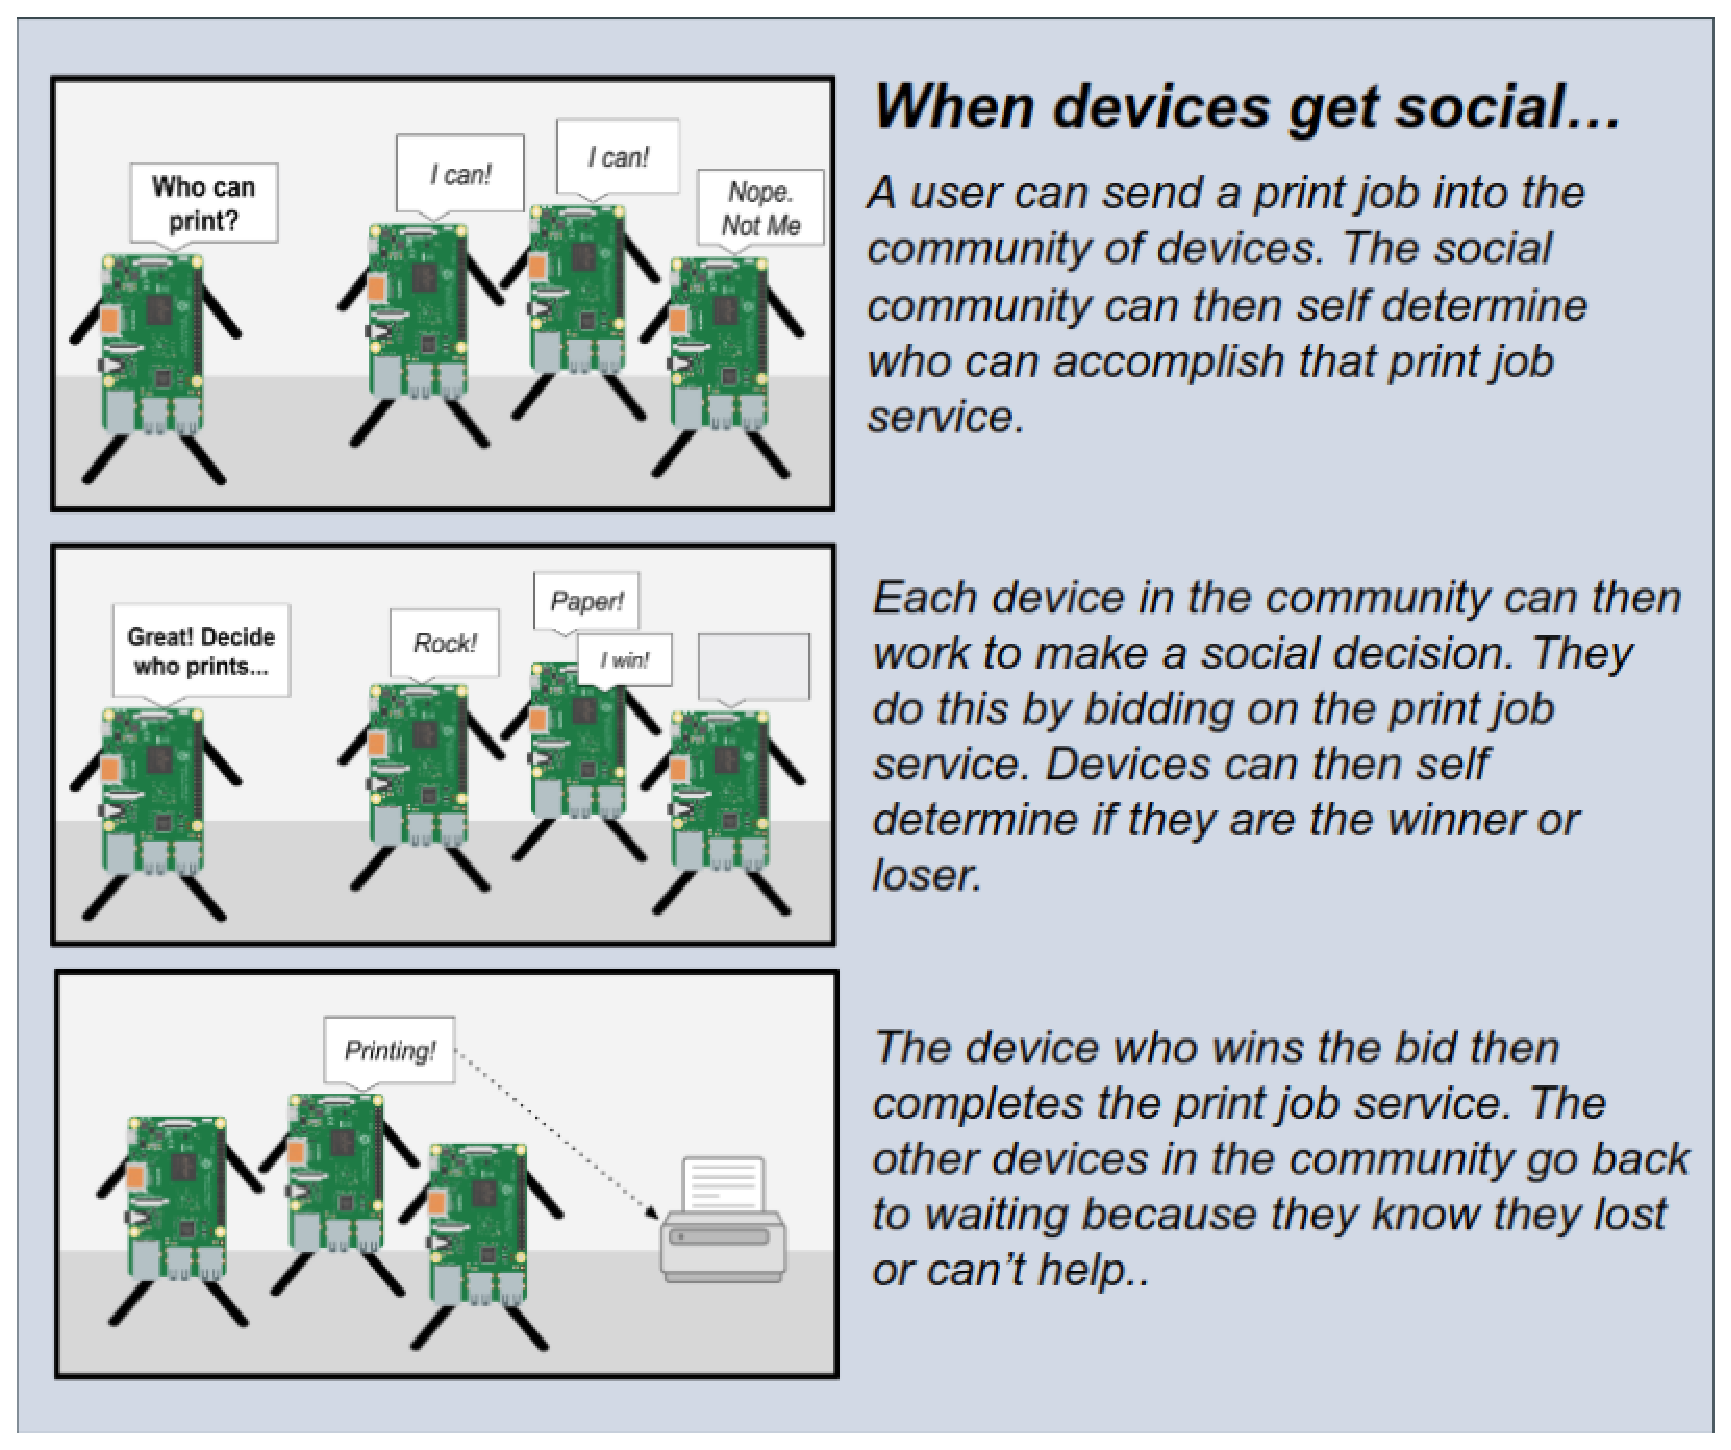
\includegraphics[scale=0.45]{social}
    \caption{This image illustrates how our nodes are able to make social decisions in order to accomplish an objective}
\end{figure}

\subsection{Installation}
To setup a node you will first need a Raspberry Pi running the latest version of Raspian. Then after a fresh install you will need to complete the steps below.
\begin{enumerate}
    \item sudo apt-get update
    \item sudo apt-get install python-pip python-dev build-essential
    \item sudo pip install --upgrade pip
    \item sudo pip install flask npm flask-socketio flask\_cors RPi.GPIO
    \item sudo apt-get install cups
    \item sudo apt-get install python-cups
    \item clone the ROUS repository to home dir (/home/pi/)
\end{enumerate}
Now you can open up a terminal and navigate to projectrous/ROUS/install/node/. Then run the commands "chmod +x install\_node.sh" followed by "./install\_node". Once that process completes your done installing. If you want you can delete the cloned repo now because a copy with only the necessary files has been copied over.
\subsection{Running}
If you installed using the install node script then open up a new terminal or navigate to /home/pi/ and then run the command "make". This will start up a node and that node will then begin listening for messages.

Another way to start a node is to just clone the repo and then open a terminal and navigate to projectrous/ROUS/ and then run the command "make node". This will do the same as above by starting a node and then that node will begin listening for messages.

\subsection{Special Requirements}
Our system runs on Raspberry Pi's and has only been tested running on Raspbian. We support Raspberry Pi Zero W's and Raspberry Pi 3b's. 

\section{Recommended Technical Resources for Learning More}
\subsection{Web Sites}
\begin{enumerate}
    \item \textbf{Python:} "https://docs.python.org/3/library/index.html"
    \item \textbf{Python Flask:} "http://flask.pocoo.org/"
    \item \textbf{SocketIO:} "https://socket.io/"
    \item \textbf{ReactJS:} "https://reactjs.org/"
    \item \textbf{NodeJS:} "https://nodejs.org/en/"
    %\item \textbf{Codecademy:} "https://www.codecademy.com/"
    \item \textbf{Raspbian:} "https://www.raspberrypi.org/downloads/raspbian/"
    \item \textbf{Git Repo:} "https://github.com/proutyio/projectrous"
    \item \textbf{React Bootstrap:} "https://react-bootstrap.github.io/"
    %\item \textbf{w3schools:} "https://www.w3schools.com/"
    %\item \textbf{dotcms:} "https://dotcms.com/blog/post/everything-you-need-to-know-about-single-page-applications"
    
\end{enumerate}

% Conclusions and Reflections (each team member answers all questions individually)
% What technical information did you learn?
% What non-technical information did you learn?
% What have you learned about project work?
% What have you learned about project management?
% What have you learned about working in teams?
% If you could do it all over, what would you do differently?
% Be honest here -- no B.S.
% Appendix 1: Essential Code Listings. You don't have to include absolutely everything, but if someone wants to understand your project, there should be enough here to learn from. If you worked within a larger project, something like a patch file might be a good way to go.
% Appendix 2: Anything else you want to include. Photos, etc.
\section{Conclusions and Reflections}
\subsection{Hayden}
\subsubsection{Technical Information Learned}
In this section I will detail the technical information I learned from working on this project throughout the year.
\begin{itemize}
    \item \textbf{Bootstrap:} Using Bootstrap for quick makeovers of your site can be very beneficial and time saving
    \item \textbf{JavaScript:} I learned how to implement JavaScript in an actual project where it
    \item \textbf{JSON:} I learned about JSON objects and how versatile using a key value pair can be when communicating between programs
    \item \textbf{Multicast:} Multicast broadcasting works differently than I originally thought; it just broadcasts to anything connected to an address regardless of port and not a group of devices like i originally thought
    \item \textbf{NodeJS:} I learned how to use NodeJS as a server side environment
    \item \textbf{ReactJS:} Learning react components, inheritance, props, and everything coming along with ReactJS to create a single page application was very intricate and helpful for the future 
    \item \textbf{SocketIO:} Sometimes going straight to sockets really helps when timing is a factor and you cannot have delay in receiving and showing received content
\end{itemize}
\subsubsection{Non-Technical Information Learned}
In this section I will detail the non-technical information I learned from working on this project throughout the year. Many of the things I learned involved finding new things and being ready for all kinds of things within the project. 
\begin{itemize}
    \item \textbf{Creativity:} Many problems required a lot of creative thinking to find ways to get around and to solve
    \item \textbf{Curiosity:} A lot of innovation and new ideas come from being curious about other ideas and projects in the same area of study, it was good to read about them
    \item \textbf{Open-minded:} When working on a project that there is some unknown, you have to be open to others ideas and find ways to incorporate them 
    \item \textbf{Prioritization:} Diving too deep into a "rabbit hole" can disrupt workflow and prioritizing tasks can really help keep workflow alive
\end{itemize}
\subsubsection{Project Work Learned}
In this section I will detail the information I learned from project work throughout the year.  On top of everything shown below, I learned that not everything you do is needed to be in the final product and that the final product would not be the same whether all of your contributions were included or not. 
\begin{itemize}
    \item \textbf{Codesandbox.io:} An online code editor for many JS languages that can help in development of applications and connects straight to GitHub
    \item \textbf{LaTex:} Using LaTex actually turned out to be helpful in the end and I should have put more effort into learning it earlier
    \item \textbf{Long Hours:} There are going to be some long hours in projects ahead and you have to expect them
    \item \textbf{Starting Early:} Getting a jump on projects early not only allows you to have more free time but allows you to incorporate more fun things into your project that make you proud of your project
    \item \textbf{VSCode:} Using the VSCode IDE was probably the best project/programming decision I made and really helped with its IntelliSense
\end{itemize}

\subsubsection{Project Management Learned}
In this section I will detail the project management techniques I learned from working on this project throughout the year. There were a lot of software engineering specific as well as general tools that can really help with project management and discussion if everyone uses them.
\begin{itemize}
    \item \textbf{Calendars} Making all events in a group on calendars is the norm in the business world and are necessary for all meetings
    \item \textbf{Early Preparation:} Getting tasks for the project out early can really help keep the team on track and know what is going on
    \item \textbf{Gantt charts:} Gannt charts really help with planning ahead and time management. It also showed how wrong some predictions of the time things would take were
    \item \textbf{Git:} I learned a lot about the inner workings of Git and its version control and how to actually use different branches and merging and some problems that happen when working on a project with more than just yourself
    \item \textbf{Github:} I learned that using GitHub as a codebase was immensely useful if used correctly
    \item \textbf{Kanban:} Kanban boards are really helpful for continual delivery on the project and to assign portions to different people
    \item \textbf{Organization:} Keeping organization throughout the project was both hard, nonexistent, and very necessary
    \item \textbf{One Note:} Using this as a general note board and keeping things on here was helpful to refer back to it even when I did not think it was going to be useful information
    \item \textbf{Reserving Ahead of Time:} Learned that reserving locations and rooms in advance is really necessary if you want to get the rooms needed for meetings
    \item \textbf{SCIPAB:} Situation. Complication. Implication. Position. Action. Benefit. A very helpful model for presenting and coming up with a good problem statement
    \item \textbf{Scrum:} Much more used in industry than I thought and can be very helpful when everyone is on the same page and uses the same tools
\end{itemize}

\subsubsection{Working in Teams}
In this section I will detail the information I learned from working on a team on this project throughout the year. Small projects that only last a term or less are very different in many ways than long projects with a lot riding on them. I learned a lot of basics that I can carry with me for larger scale projects. Chief among what I have learned is the need for confrontation. I avoided confrontation like the plague all year and paid the price for it. 
\begin{itemize}
    \item \textbf{Compromising:} While compromising is a necessary tool when working in a group, doing it too much leads to lack of respect and using other methods of agreement in conjunction is the best route
    \item \textbf{Importance of Voice:} I learned changing how you talk to different kinds of people can really change the outcome of the conversation
    \item \textbf{Communication:} I learned just how important communication and everyone being on the same page was
\end{itemize}

\subsubsection{What I would Differently}
If I were to do this year differently, I would get started earlier and find better methods of communication. I would have been more confrontational so I could get more of my ideas onto the table. I think the project would have run more smoothly if we had sat with each other and worked on the project together more often. I would have committed my changes more often and tried to communicate better. Another change I would have made would have been to attend more office hours to make sure that what I was doing was correct with the documents. Lastly, I would have kept up more with my one note entries and marked what I did on there every day as opposed to just my weekly updates.
% Conclusions and Reflections (each team member answers all questions individually)
% What technical information did you learn?
% What non-technical information did you learn?
% What have you learned about project work?
% What have you learned about project management?
% What have you learned about working in teams?
% If you could do it all over, what would you do differently?
% Be honest here -- no B.S.

% Appendix 1: Essential Code Listings. You don't have to include absolutely everything, but if someone wants to understand your project, there should be enough here to learn from. If you worked within a larger project, something like a patch file might be a good way to go.
% Appendix 2: Anything else you want to include. Photos, etc.


\subsection{Kyle}
\subsubsection{Technical Information Learned}
I learned a lot of things in order to complete this project. Most technologies and tools used were new to me and it was a lot of fun diving in head first. I feel like I came out of this experience with a lot of new knowledge that will help me in future projects.
\begin{itemize}
    \item \textbf Python Flask
    \item \textbf Multicast communication
    \item \textbf TCP communication
    \item \textbf SocketIO web sockets
    \item \textbf npm (node package manager)
    \item \textbf React
    \item \textbf Bootstrap React
\end{itemize}
\subsubsection{Non-Technical Information Learned}
There were a lot of things I learned that had nothing to do with software development. I learned about how to make better time management choices and when I need to make decisions about how I spread out my time. It was helpful to look at the cost vs the reward of how I spent my time. Learning how to deal with different stressful situation and different personalities has been very helpful.

I think overall that the professional development has been the best thing I learned. Such as how to communicate in a professional environment using emails, Slack, and Skype.
\begin{itemize}
    \item \textbf Time Management
    \item \textbf Stress Management
    \item \textbf Skype Meetings
    \item \textbf Project Documentation
    \item \textbf Translating client requirements into a product
    \item \textbf Cost vs Reward
    \item \textbf Professional email exchange
\end{itemize}
\subsubsection{Project Management Learned}
Overall I learned a lot about project management and how to deal with certain situations. I learned about how to better handle situations. Lonnie was a great mentor and shared a lot of advice when it comes to project management and just dealing with a stressful group dynamic in general. 
\begin{itemize}
    \item \textbf SCIPAB (Situation, Complication, Implication, Position, Action, Benefit)
    \item \textbf Agile principles - scrum, scrum master
    \item \textbf Accountability
    \item \textbf Communication
\end{itemize}

\subsubsection{Working in Teams}
Throughout the many group projects I have done, working in teams always has some strengths and weaknesses, and each group dynamic is different. Communication is always key to any relationship or group dynamic. An import aspect I find is when teammates discover that they are not just accountable to themselves but to the other teammates. If they are not interested and put in no effort to have new ideas or constructive input during meeting then that can have a negative affect on the group as a whole. 

Working in teams requires that other teammates do research and independent work on their own. Then during team meetings all group members are educated on the topic and are prepared with different ideas. It requires that even if things are not communicated directly that the other teammates use the other resources around to discover that information on their own. Specifically with a software project all code is on GitHub and easily readable by all teammates. If I teammate wants to discover all the progress of another teammate without having to burden that other teammate all the time, then using GitHub to view recent code commits is very helpful.

In the end working in teams can be difficult if the other teammates are uninterested or feel like "someone else will just do it". All teammates need to take personal charge of the project. Overall teams are a great way to spread the work around and to help collaborate on ideas. When all teammates take person responsibility in the production and completion of the project then group work is awesome.

\subsubsection{What I would Differently}
There are a lot of things I would do differently. I can't change other peoples motivation though. To start I should have made a better effort to understand everyone strengths and weaknesses. 

I would set up individual goals and then hold people accountable to those. Each member would be required to complete the parts they said they would complete by a certain time and then be required to show the group the progress they made and how those features are working with the rest of the overall project.

Making an effort to make sure everyone was on the same page at the end of every week. I don't mean this in the sense that every week one person talks about the goals of the project and what was done. Every group member should be required to share what they did, how it integrates in the project, what problems they had, and what they plan on doing next. Each teammate should have a high level view of what all other teammates are working on. 

Overall I would communicate more and take steps to ensure that all teammates were correctly motivated and felt like they had the knowledge and tools to complete the task.


\newpage
\section{Appendix 1: Essential Code Listings}
https://github.com/proutyio/projectrous/tree/master/ROUS
\section{Appendix 2: Final Look}
\begin{figure}[H]
\centering
    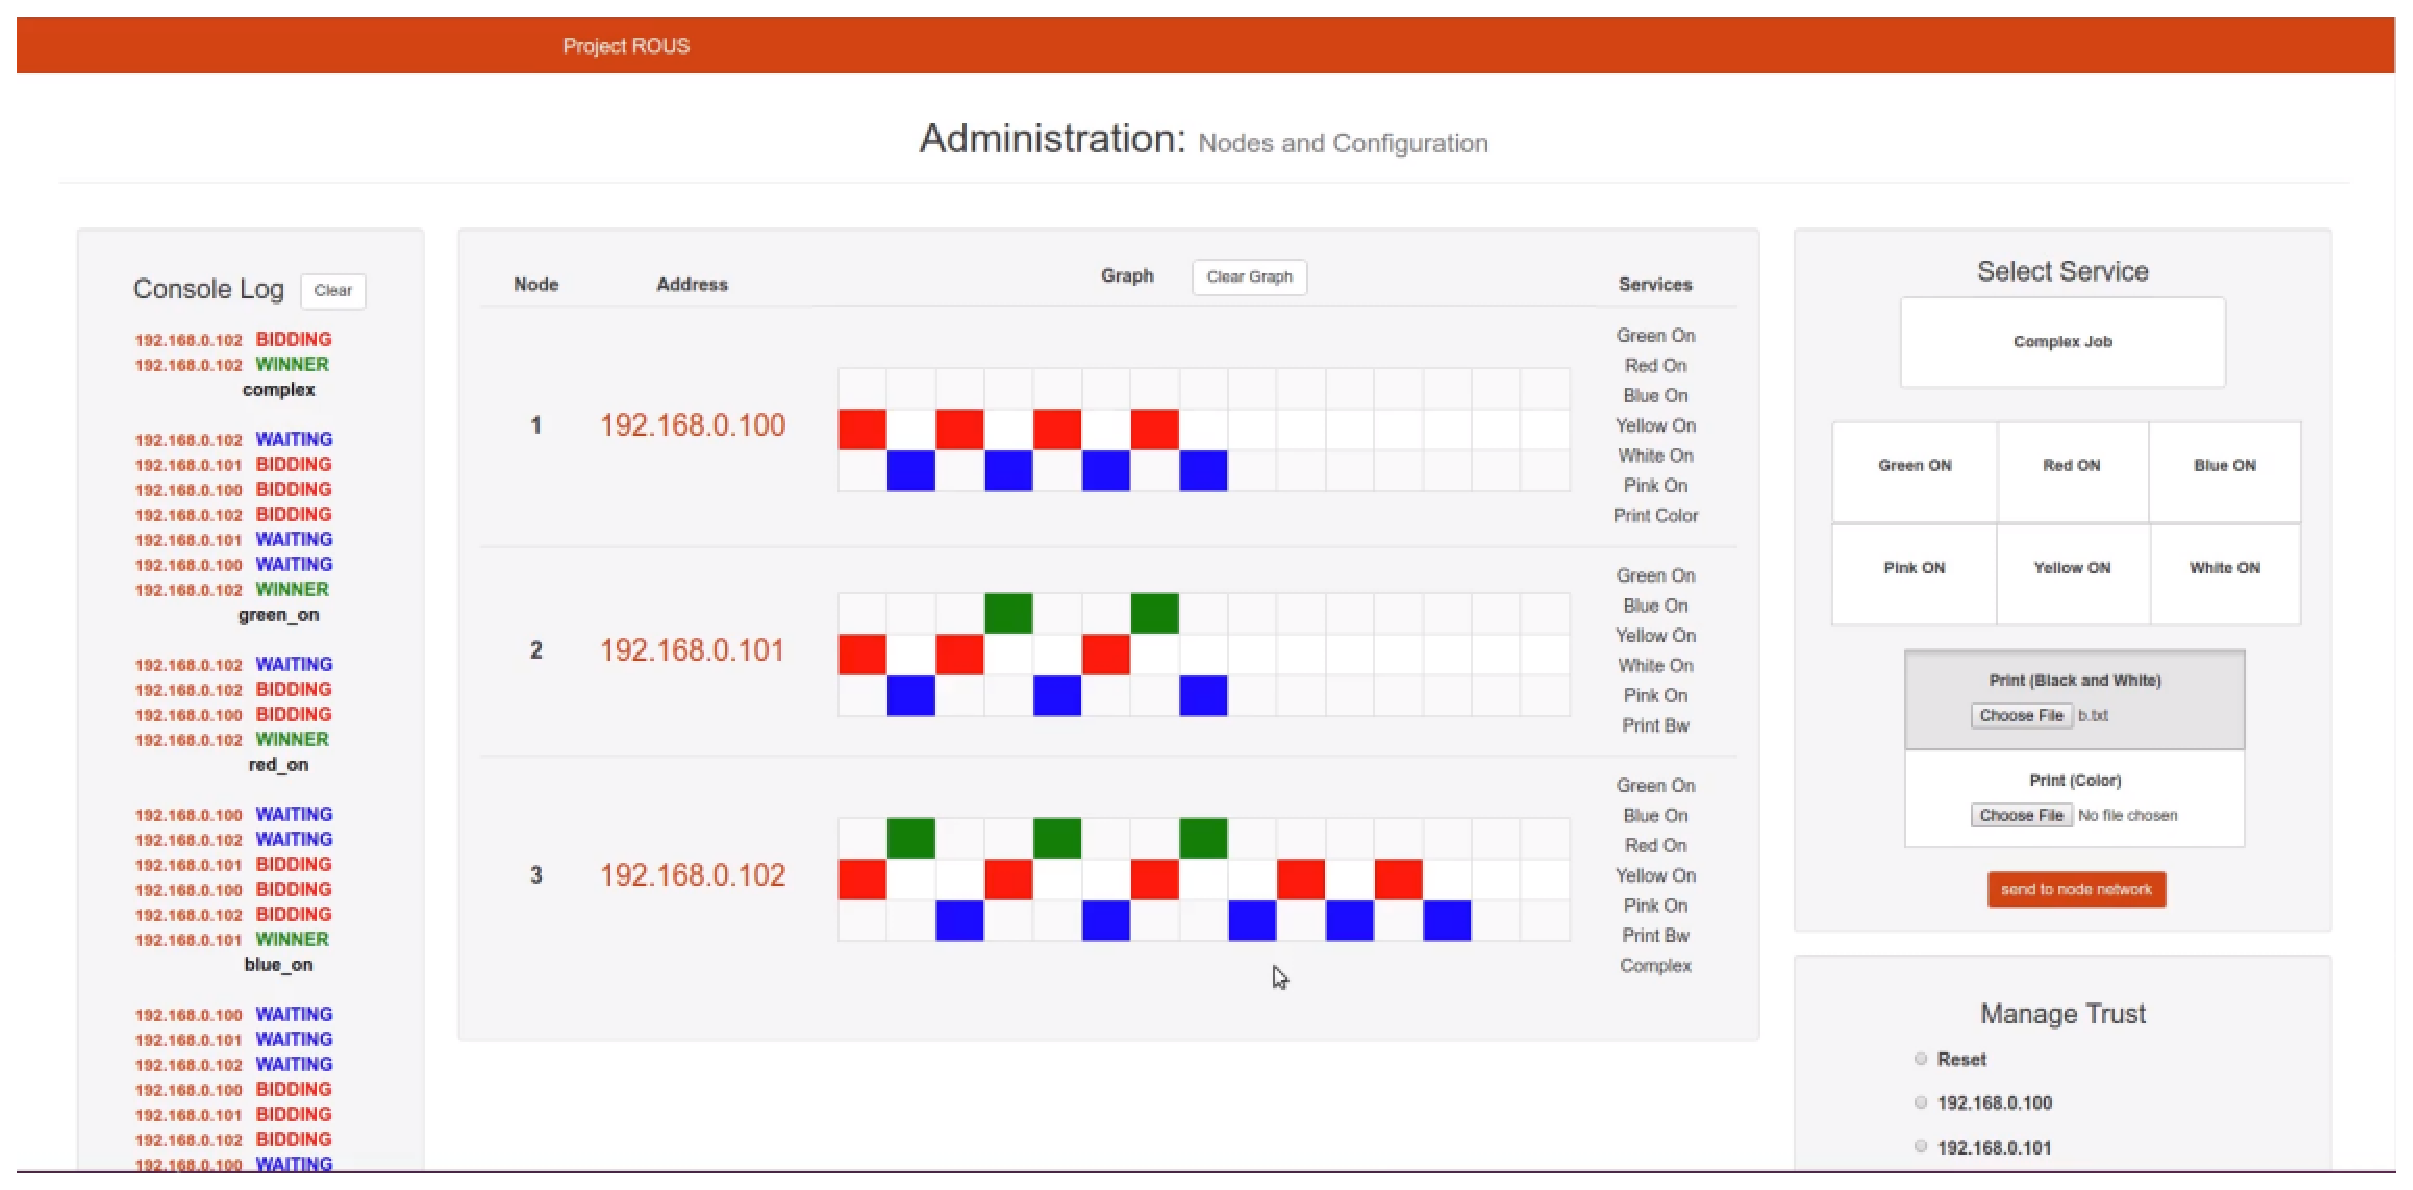
\includegraphics[scale=0.45]{img1}
    \caption{This is a screenshot showing the administrator interface. You can see nodes allow with the current state of the system}
\end{figure}
\begin{figure}[H]
\centering
    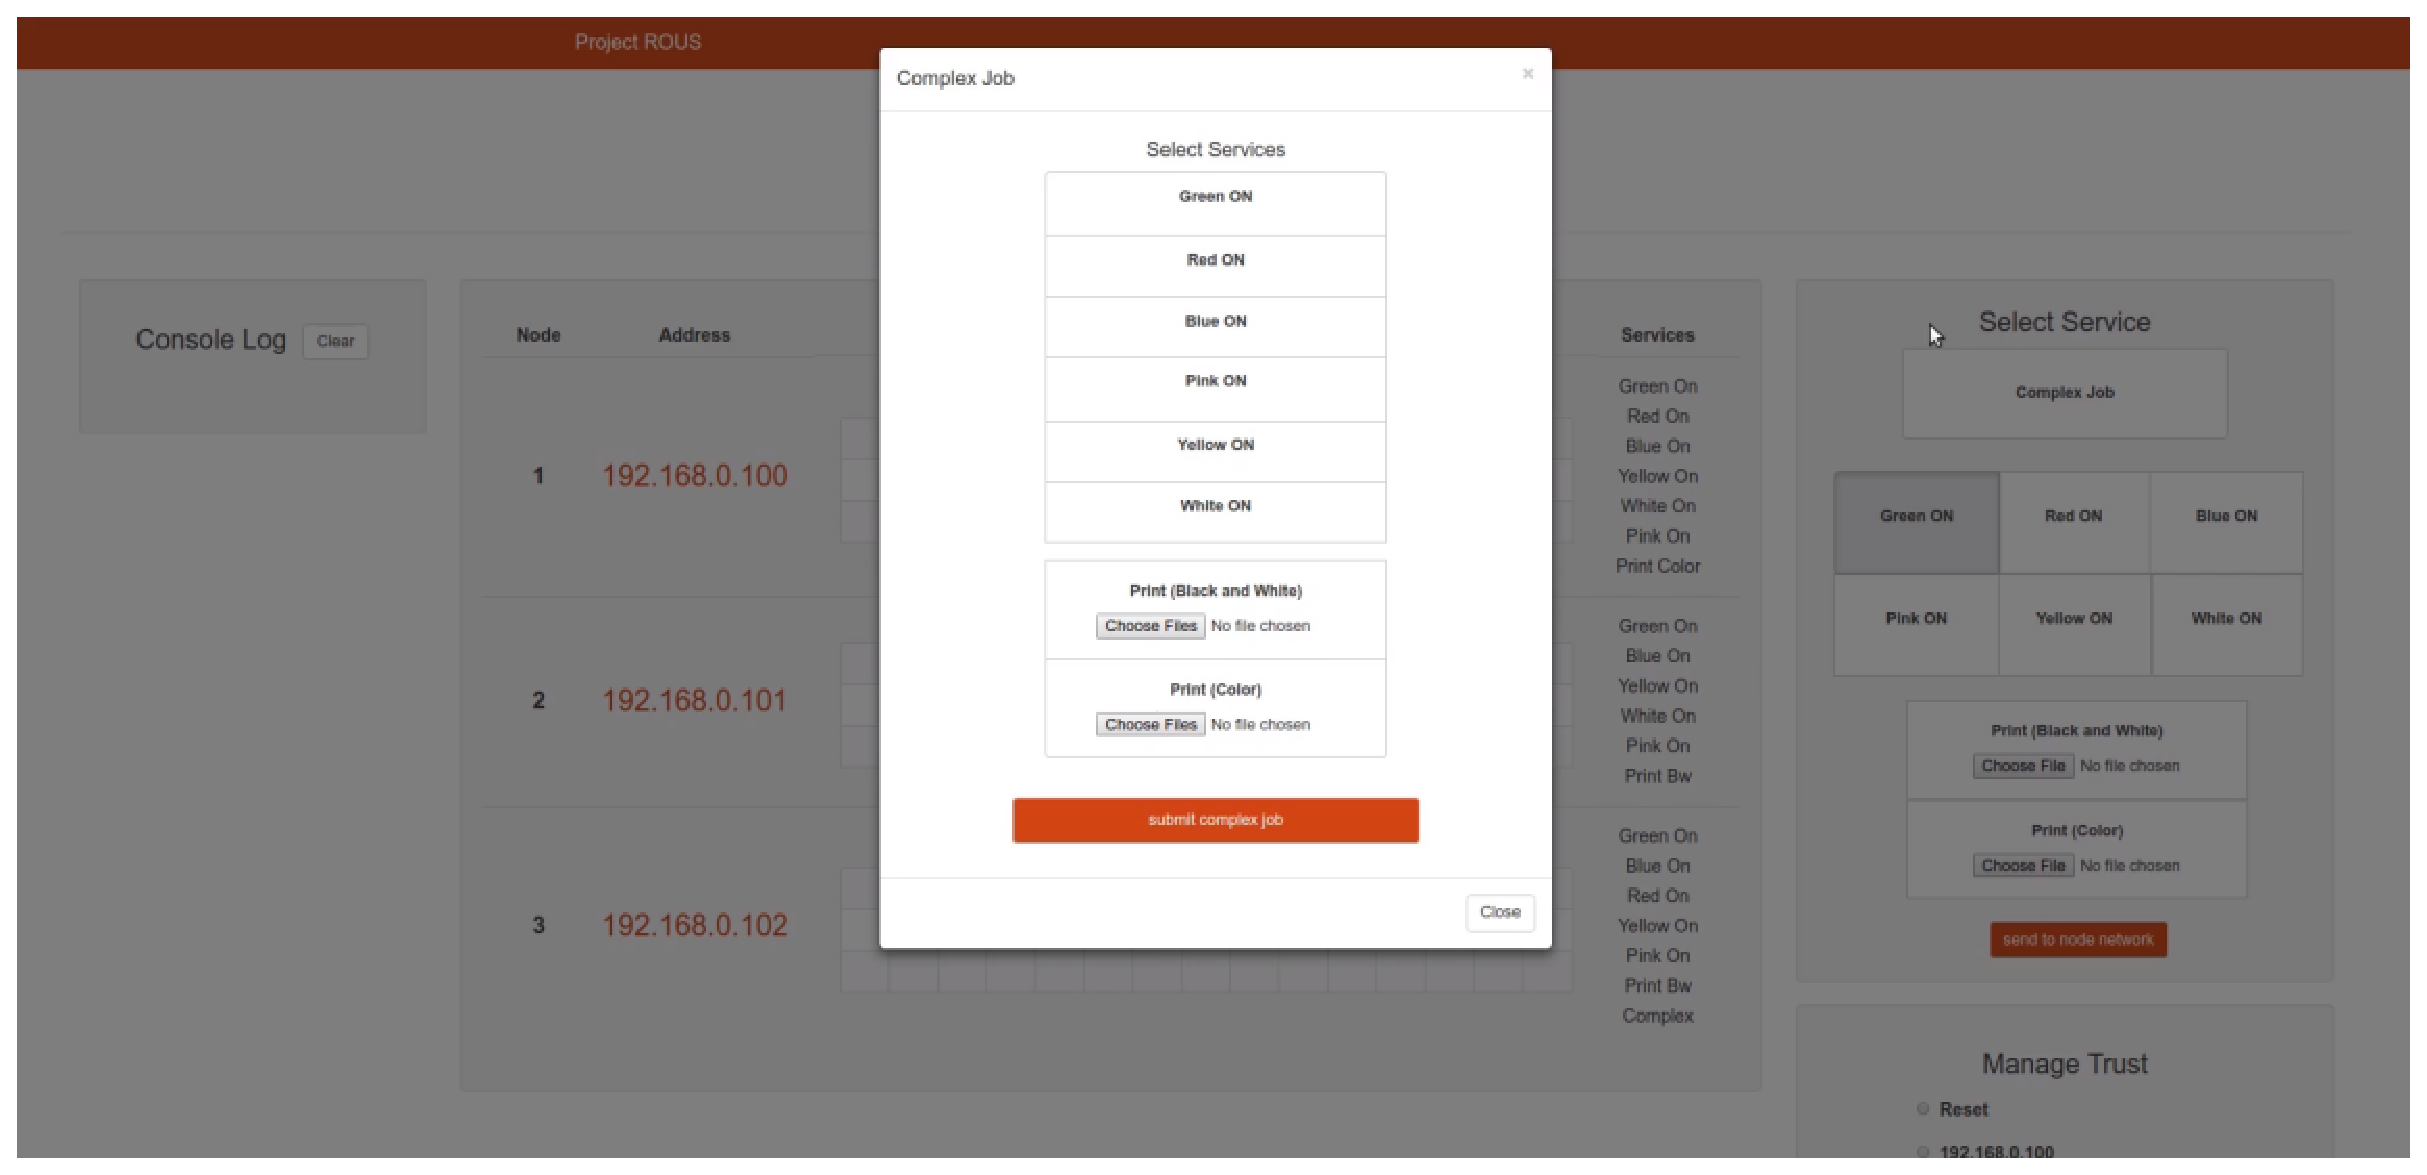
\includegraphics[scale=0.45]{img2}
    \caption{Above shows a popup window on the administrator interface of the user interface. This window allows the user to input a complex service}
\end{figure}
\begin{figure}[H]
\centering
    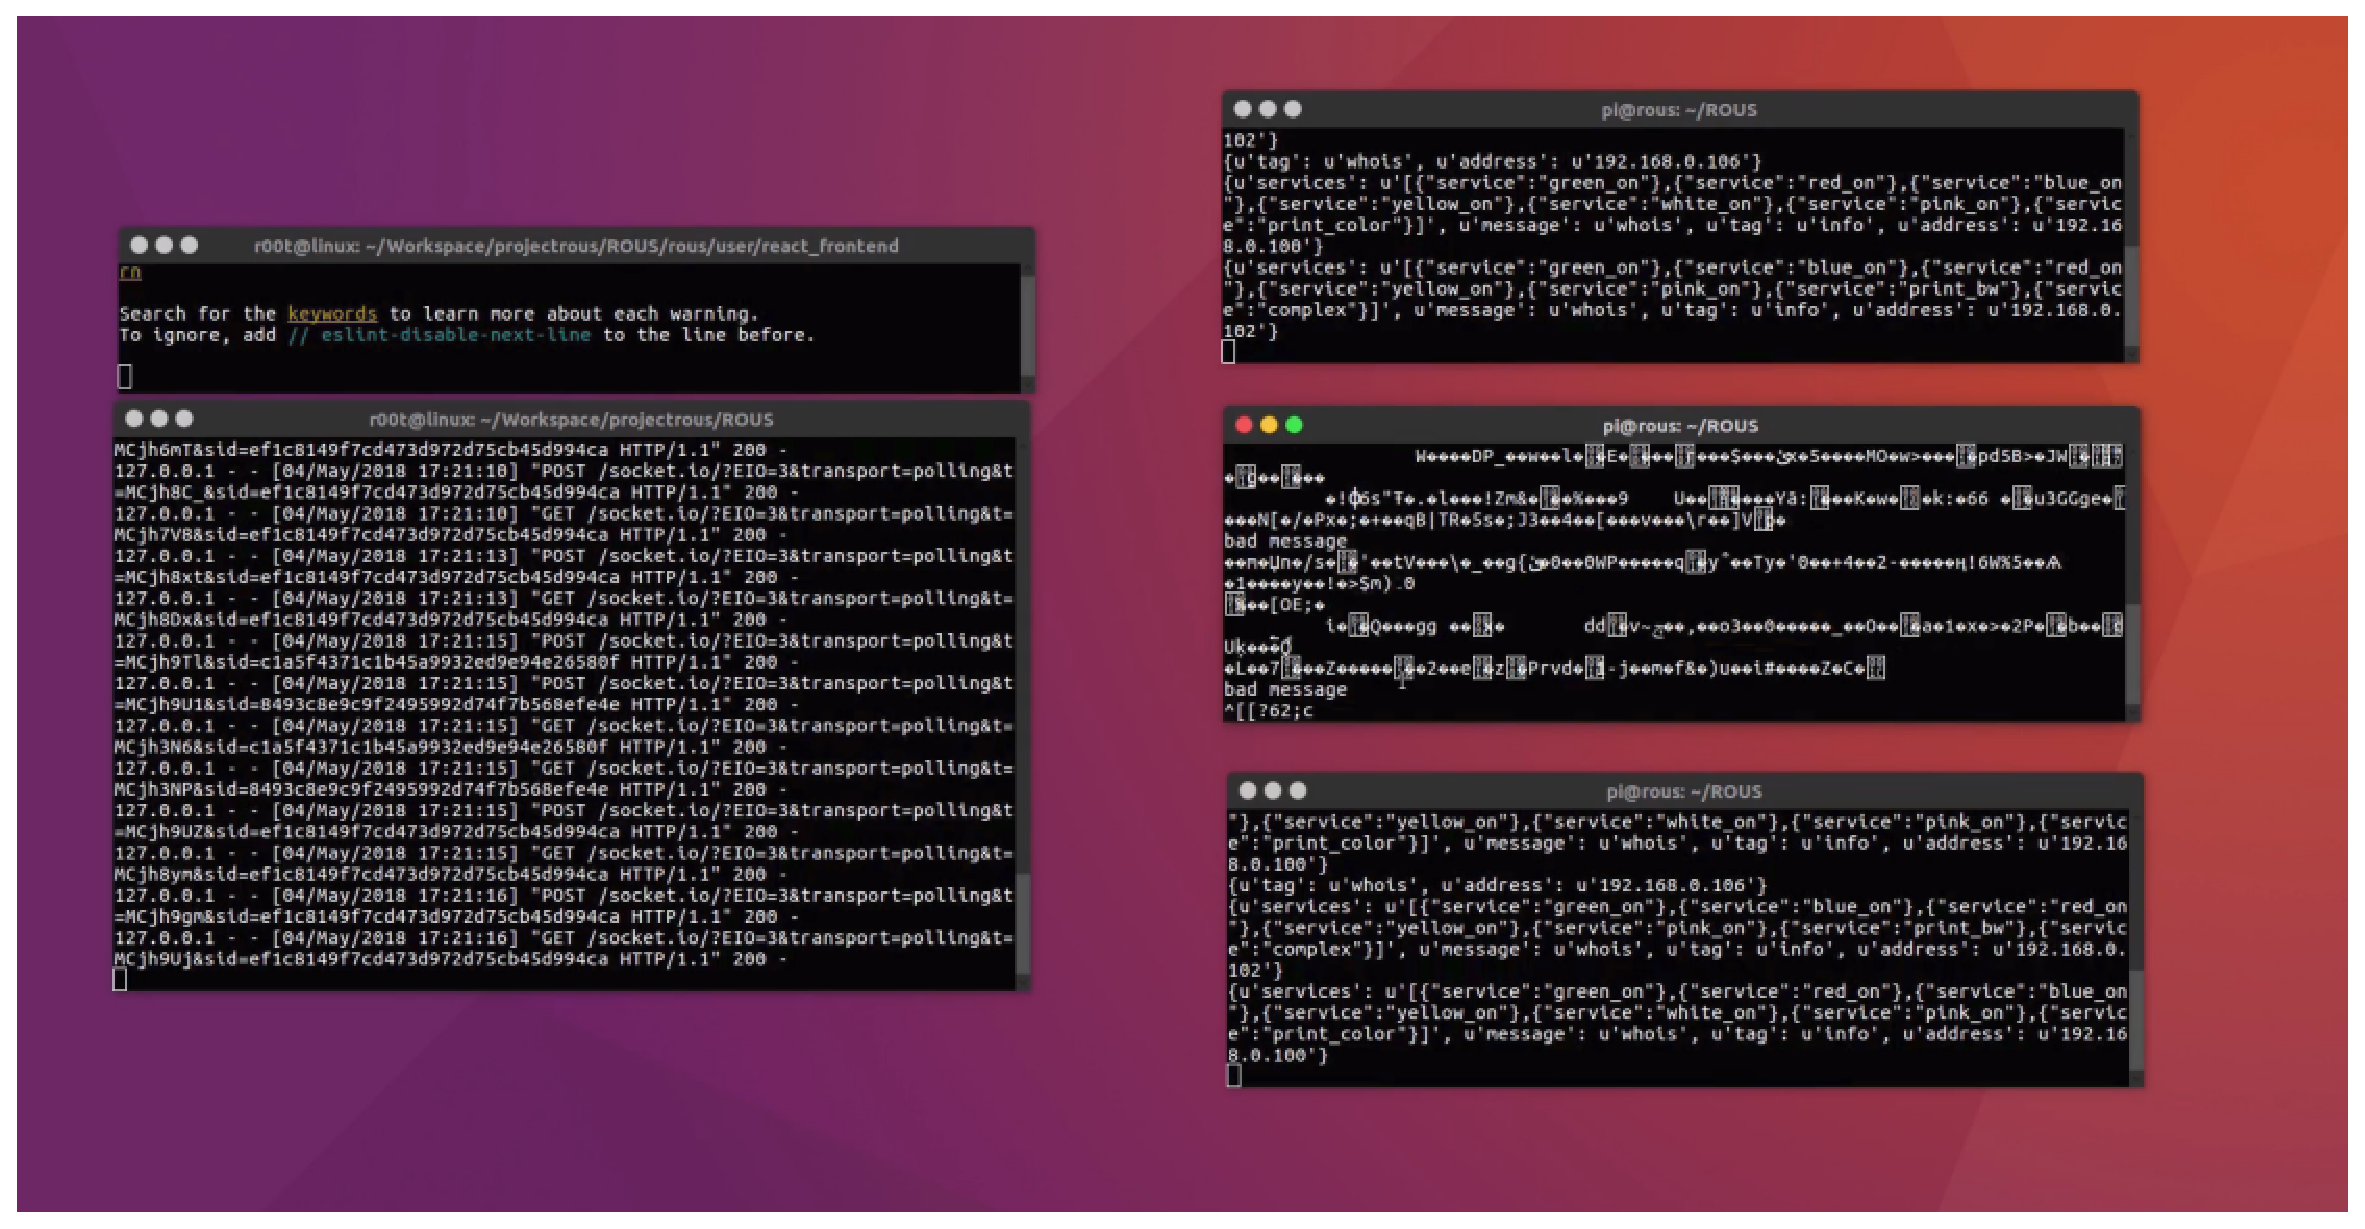
\includegraphics[scale=0.45]{img3}
    \caption{In this image you can see on the right hand side that we are ssh into 3 nodes and are running the node program. You can see that one node does not have the correct encryption key and is thus not in the same trust group as the other two nodes. On the left side you can see the front end and back end running that make up the user interface}
\end{figure}
\begin{figure}[H]
\centering
    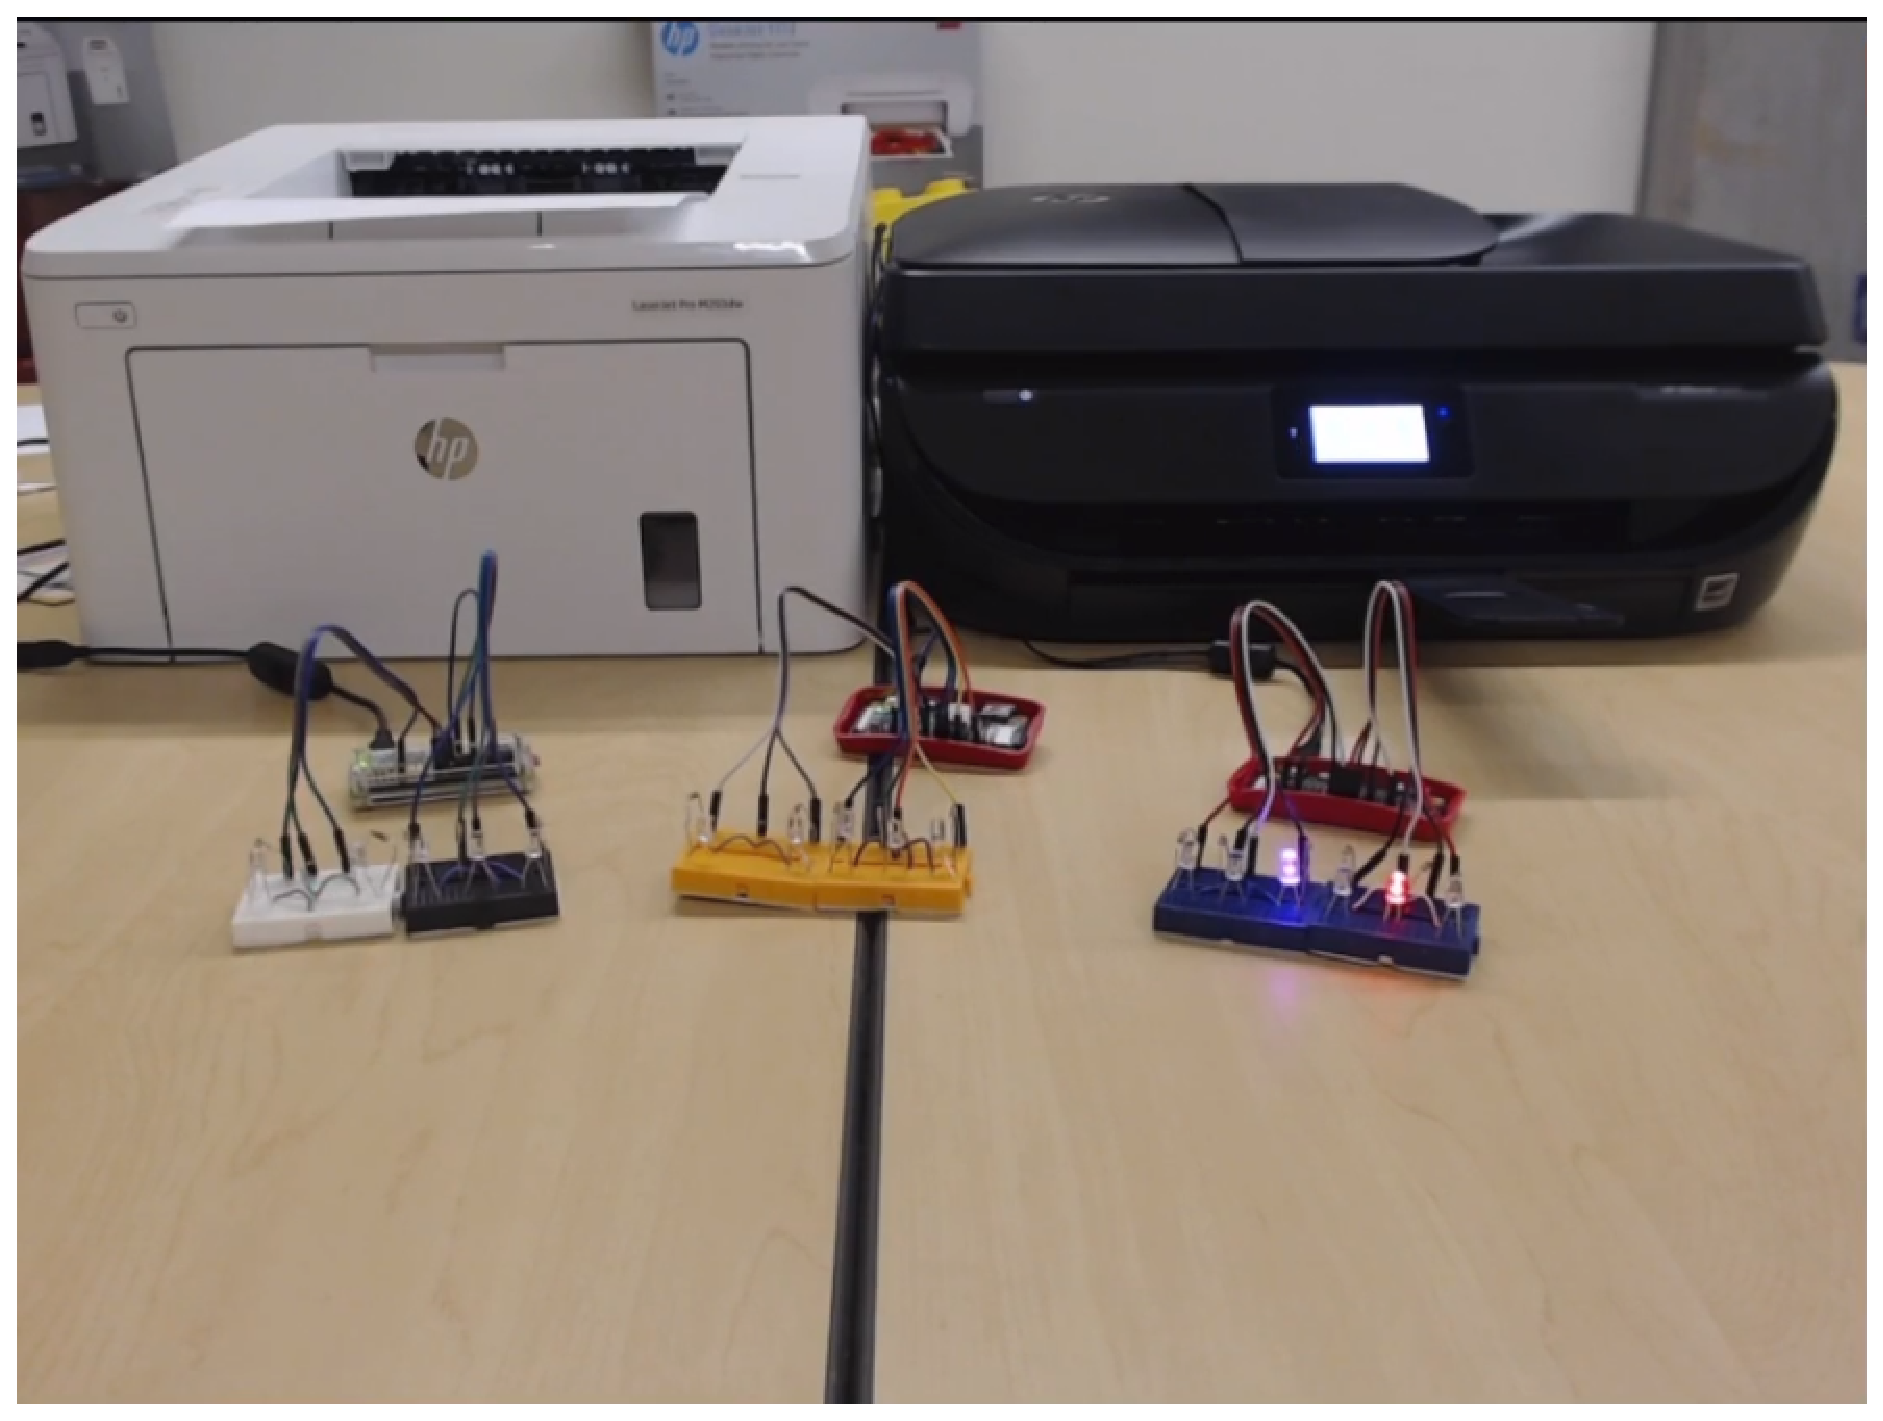
\includegraphics[scale=0.45]{setup}
    \caption{This still from a demo which demonstrated 3 nodes where each node had a one-to-one relationship with a printer and some LEDs. Nodes are collaborating on a print job objective}
\end{figure}

\newpage
\nocite{*}
\bibliographystyle{plain}
\bibliography{bibtex}


\end{document}